\documentclass{article}
\usepackage[T1]{fontenc}
\usepackage{lmodern}
\usepackage{graphicx}
\usepackage{amsmath,amssymb}
\usepackage[a4paper,margin=2cm]{geometry}
\usepackage[absolute,overlay]{textpos}
\setlength{\TPHorizModule}{1mm}
\setlength{\TPVertModule}{1mm}
\usepackage[indonesian]{babel}
\usepackage{hyperref}
\setlength{\emergencystretch}{2em}
\title{04-Kriptografi-klasik-bagian2-(2026)}
\author{pdf\_ppt\_to\_latex}
\date{}

\begin{document}

% --- unit llm 1 ---
% === Halaman 1 (llm) ===

\begin{center}
Bahan kuliah IF4020 Kriptografi

\vspace{10mm}
\Huge \textcolor{red}{04 - Kriptografi Klasik}
\large \textcolor{red}{(Bagian 2)}

\vspace{98.90mm}

\vspace{10mm}
\large Oleh: Rinaldi M

\vspace{20mm}
\textbf{Pogram Studi Teknik Informatika}\
\textbf{Sekolah Teknik Elektro dan Informatika}\
\textbf{Institut Teknologi Bandung}\
\textbf{2026}
\end{center}

% deskripsi: Ilustrasi mesin kriptografi klasik berupa silinder huruf yang dapat diputar untuk enkripsi.
% bbox normalisasi: [0.0470, 0.4330, 0.3030, 0.7660]
\begin{textblock*}{53.76mm}(9.87mm,128.60mm)
\noindent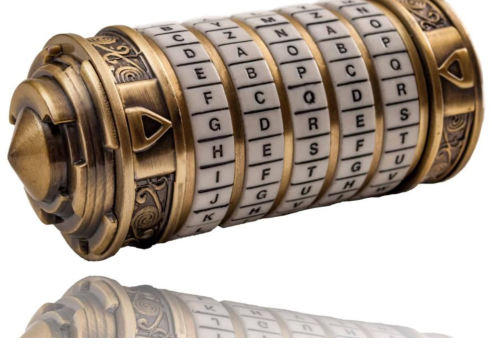
\includegraphics[width=53.76mm,height=98.90mm]{images/llm/page_001_img_01.png}%
\end{textblock*}

\newpage

% --- unit llm 2 ---
% === Halaman 2 (llm) ===

\section*{A. Cipher Abjad-Tunggal (monoalphabetic cipher)}

\begin{itemize}
    \item \textit{Monoalpaphetic cipher}: kelompok cipher substitusi yang mengganti satu huruf dengan satu huruf yang lain
    \item \textit{Caesar cipher} adalah salah satu \textit{cipher} abjad-tunggal dengan melakukan substitusi huruf berdasarkan hasil pergeseran huruf-huruf alfabet sejauh $k$ huruf. Namun \textit{Caesar Cipher} bukan satu-satunya \textit{cipher} abjad-tunggal.
    \item Secara umum, kita dapat membentuk tabel subtitusi sembarang. Jumlah kemungkinan tabel substitusi yang dapat dibuat pada sembarang \textit{cipher} abjad-tunggal adalah sebanyak
    \[ 26! = 403.291.461.126.605.635.584.000.000 \]
    karena ada $26!$ cara mempermutasikan 26 huruf alfabet.
\end{itemize}

\newpage

% --- unit llm 3 ---
% === Halaman 3 (llm) ===

\begin{itemize}
  \item Tabel substitusi dapat dibentuk secara acak seperti contoh berikut:
\end{itemize}
\vspace{10mm}
\begin{itemize}
  \item Atau berdasarkan kalimat kunci yang mudah diingat:
\end{itemize}
\textbf{Contoh:} \texttt{di bawah sinar bulan purnama hati resah jadi senang}

\vspace{31.19mm}

\textbf{Buang duplikasi huruf menjadi:} \texttt{dibawhsnrulpmtejg}

\textbf{Sambung dengan huruf lain yang belum ada:}

\texttt{dibawhsnrulpmtejgcfkoqvwxyz}

\textbf{Tabel substitusi yang dihasilkan:}

\begin{tabular}{ll}
Plainteks : & A B C D E F G H I J K L M N O P Q R S T U V W X Y Z \\
Cipherteks : & \textbf{D I B A W H S N R U L P M T E J G C F K O V W X Y Z}
\end{tabular}

% deskripsi: Tabel substitusi huruf acak yang memetakan Plainteks ke Cipherteks
% bbox normalisasi: [0.1900, 0.2050, 0.9050, 0.3100]
\begin{textblock*}{150.15mm}(39.90mm,60.88mm)
\noindent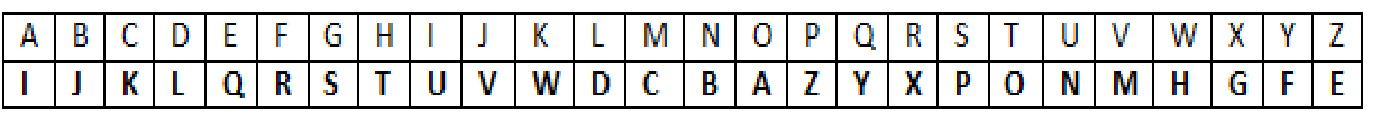
\includegraphics[width=150.15mm,height=31.19mm]{images/llm/page_003_img_01.png}%
\end{textblock*}

\newpage

% --- unit llm 4 ---
% === Halaman 4 (llm) ===

\section*{Kriptanalisis Cipher Abjad-Tunggal}

\begin{itemize}
    \item Kelemahan \textit{cipher} abjad-tunggal: tidak dapat menyembunyikan hubungan statistik antara plainteks dengan cipherteks.
    \begin{itemize}
        \item Huruf yang sama dienkripsi menjadi huruf cipherteks yang sama
        \item Huruf yang sering muncul di dalam plainteks, juga sering muncul di dalam huruf cipherteksnya yang berkoresponden.
        \item artinya struktur statistik bahasa masih muncul di dalam cipherteks
    \end{itemize}
    \item Oleh karena itu, cipherteks dapat didekripsi tanpa mengetahui kuncinya sekalipun dengan menggunakan \textbf{teknik analisis frekuensi}.
\end{itemize}

\newpage

% --- unit llm 5 ---
% === Halaman 5 (llm) ===

\section*{Teknik Analisis Frekuensi}

\begin{itemize}
    \item Pada \textit{cipher} abjad-tunggal, perulangan huruf di dalam plainteks tercermin pula pada perulangan huruf cipherteksnya.
    \item Artinya, huruf yang sering muncul di dalam plainteks, maka huruf cipherteksnya juga sering muncul.
    \item Hubungan statistik antara huruf-huruf di dalam plainteks dengan huruf-huruf di dalam cipherteks menjadi peluang bagi kriptanalis untuk memecahkan cipherteks tanpa mengetahui kunci yang digunakan.
    \item Dengan memanfaatkan tabel frekuensi kemunculan huruf, pasangan huruf (bigram), dan tiga huruf (trigram) di dalam suatu bahasa natural, kriptanalis dapat dapat mencari tabel substitusi huruf plainteks menjadi huruf cipherteks dengan
\end{itemize}

\newpage

% --- unit llm 6 ---
% === Halaman 6 (llm) ===

\vspace{166.32mm}

\textbf{Tabel} Frekuensi kemunculan (relatif) huruf-huruf dalam teks Bahasa Inggris (sampel mencapai 300.000 karakter di dalam sejumlah novel dan suratkabar)

% deskripsi: Tabel distribusi frekuensi relatif huruf-huruf alfabet Inggris.
% bbox normalisasi: [0.0300, 0.3000, 0.5300, 0.8600]
\begin{textblock*}{105.00mm}(6.30mm,89.10mm)
\noindent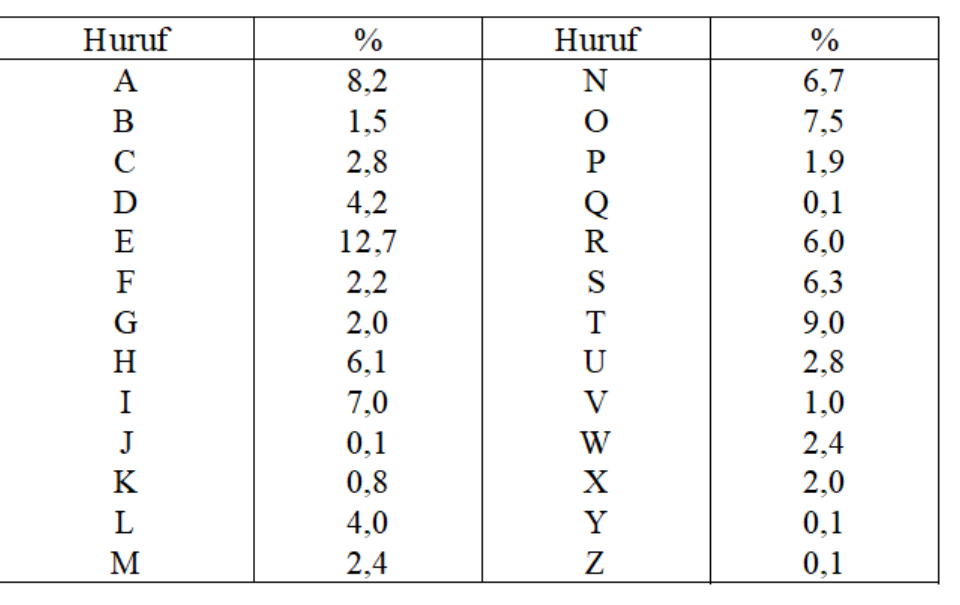
\includegraphics[width=105.00mm,height=166.32mm]{images/llm/page_006_img_01.png}%
\end{textblock*}

% deskripsi: Grafik batang yang menunjukkan frekuensi relatif kemunculan setiap huruf alfabet Inggris.
% bbox normalisasi: [0.5600, 0.2100, 0.9600, 0.9100]
\begin{textblock*}{84.00mm}(117.60mm,62.37mm)
\noindent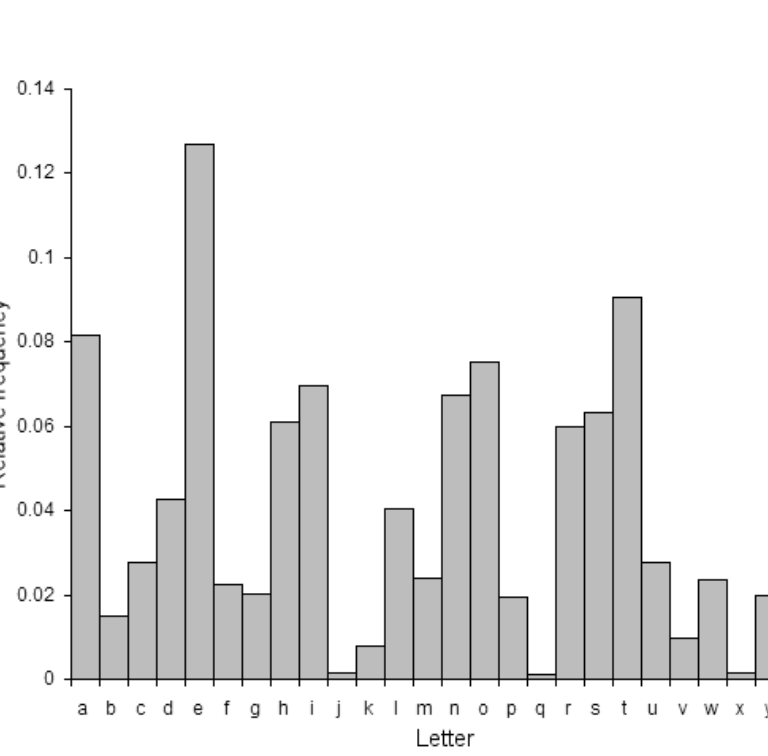
\includegraphics[width=84.00mm,height=207.90mm]{images/llm/page_006_img_02.png}%
\end{textblock*}

\newpage

% --- unit llm 7 ---
% === Halaman 7 (llm) ===

\vspace{163.35mm}

\begin{itemize}
    \item Top 10 huruf yang sering muncul dalam teks Bahasa Inggris: E, T, A, O, I, N, S, H, R, D, L, U
    \vspace{10mm}
    \item Top 10 huruf \textit{bigram} yang sering muncul dalam teks B. Inggris: TH, HE, IN, EN, NT, RE, ER, AN, TI, dan ES
    \item Top 10 huruf \textit{trigram} yang sering muncul dalam teks B. Inggris: THE, AND, THA, ENT, ING, ION, TIO, FOR, NDE, dan HAS
    \item Kriptanalis menggunakan tabel frekuensi kemunculan huruf dalam B. Inggris sebagai kakas bantu melakukan dekripsi.
    \item Misalnya, jika huruf ``R'' paling sering muncul di dalam cipherteks, maka kemungkinan besar itu adalah huruf ``E'' di dalam plainteksnya.
\end{itemize}

% deskripsi: Grafik batang yang menunjukkan frekuensi relatif kemunculan setiap huruf dalam alfabet Bahasa Inggris, dengan sumbu x berupa huruf (a-z) dan sumbu y berupa Relative Frequency (in percent).
% bbox normalisasi: [0.5400, 0.2200, 0.9600, 0.7700]
\begin{textblock*}{88.20mm}(113.40mm,65.34mm)
\noindent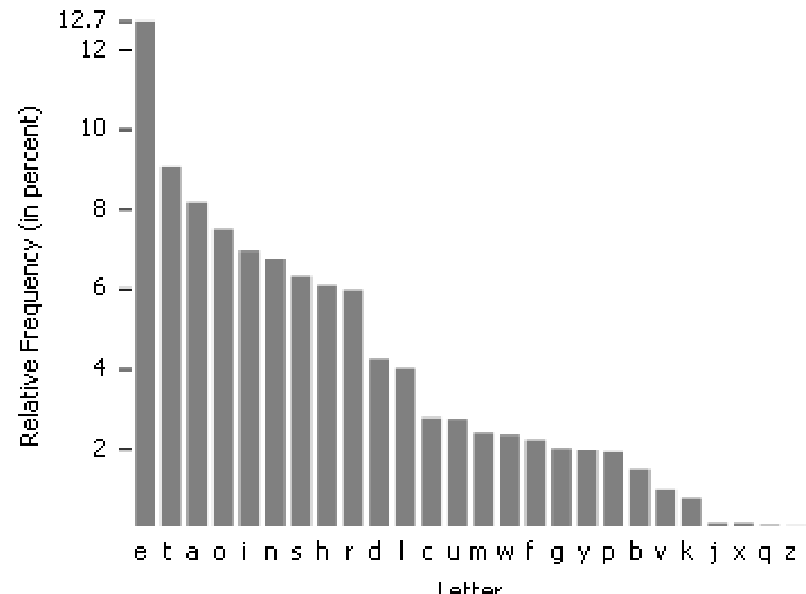
\includegraphics[width=88.20mm,height=163.35mm]{images/llm/page_007_img_01.png}%
\end{textblock*}

\newpage

% --- unit llm 8 ---
% === Halaman 8 (llm) ===

\section*{Bigram Frequencies}
\begin{tabular}{lll}
TH : 2.71 & EN : 1.13 & NG : 0.89 \\
HE : 2.33 & AT : 1.12 & AL : 0.88 \\
IN : 2.03 & ED : 1.08 & IT : 0.88 \\
ER : 1.78 & ND : 1.07 & AS : 0.87 \\
AN : 1.61 & TO : 1.07 & IS : 0.86 \\
RE : 1.41 & OR : 1.06 & HA : 0.83 \\
ES : 1.32 & EA : 1.00 & ET : 0.76 \\
ON : 1.32 & TI : 0.99 & SE : 0.73 \\
ST : 1.25 & AR : 0.98 & OU : 0.72 \\
NT : 1.17 & TE : 0.98 & OF : 0.71 \\
\end{tabular}

\vspace{10mm}

\section*{Trigram Frequencies}
\begin{tabular}{lll}
THE : 1.81 & ERE : 0.31 & HES : 0.24 \\
AND : 0.73 & TIO : 0.31 & VER : 0.24 \\
ING : 0.72 & TER : 0.30 & HIS : 0.24 \\
ENT : 0.42 & EST : 0.28 & OFT : 0.22 \\
ION : 0.42 & ERS : 0.28 & ITH : 0.21 \\
HER : 0.36 & ATI : 0.26 & FTH : 0.21 \\
FOR : 0.34 & HAT : 0.26 & STH : 0.21 \\
THA : 0.33 & ATE : 0.25 & OTH : 0.21 \\
NTH : 0.33 & ALL : 0.25 & RES : 0.21 \\
INT : 0.32 & ETH : 0.24 & ONT : 0.20 \\
\end{tabular}

\newpage

% --- unit llm 9 ---
% === Halaman 9 (llm) ===

\vspace{180.28mm}

\begin{itemize}
  \item Perbandingan: top 10 huruf yang paling sering muncul dalam Bahasa Indonesia:
\end{itemize}
\vspace{5mm}

% deskripsi: Tabel frekuensi kemunculan 10 huruf teratas dalam Bahasa Indonesia beserta persentase peluangnya.
% bbox normalisasi: [0.3670, 0.2160, 0.5210, 0.8230]
\begin{textblock*}{32.34mm}(77.07mm,64.15mm)
\noindent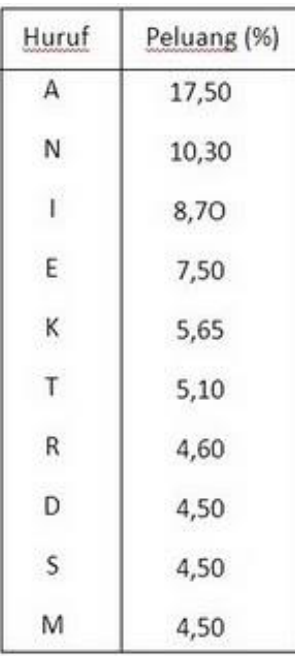
\includegraphics[width=32.34mm,height=180.28mm]{images/llm/page_009_img_01.png}%
\end{textblock*}

\newpage

% --- unit llm 10 ---
% === Halaman 10 (llm) ===

Langkah-langkah kriptanalisis dengan teknik analisis frekuensi adalah sbb:

\begin{enumerate}
  \item Hitung frekuensi kemunculan relatif huruf-huruf di dalam cipherteks.
  \item Bandingkan hasil langkah 1 dengan tabel frekuensi kemunculan huruf. Mengingat huruf yang paling sering muncul dalam teks Bahasa Inggris adalah huruf E, maka huruf yang paling sering muncul di dalam cipherteks kemungkinan besar berpadanan dengan huruf E di dalam plainteksnya.
  \item Langkah 2 diulangi untuk huruf dengan frekuensi terbanyak berikutnya. (biasanya hanya terpakai untuk 2 sampai 3 huruf pertama di dalam tabel frekuensi).
  \item Ulangi langah 1 dan 2 dengan menggunakan bigram, trigram, dst, yang sering muncul di dalam cipherteks.
\end{enumerate}

\newpage

% --- unit llm 11 ---
% === Halaman 11 (llm) ===

\vspace{222.75mm}

\begin{itemize}
    \item Kakas online untuk menghitung frekuensi kemunculan huruf, bigram, trigram dsb: \url{https://www.cryptool.org/en/cto/n-gram-analysis}
\end{itemize}
\vspace{10mm}

% deskripsi: Screenshot halaman web CrypTool-Online untuk analisis N-gram yang menunjukkan input teks ciphertext dan pengaturan panjang tabel serta n-gram.
% bbox normalisasi: [0.1400, 0.1800, 0.8900, 0.9300]
\begin{textblock*}{157.50mm}(29.40mm,53.46mm)
\noindent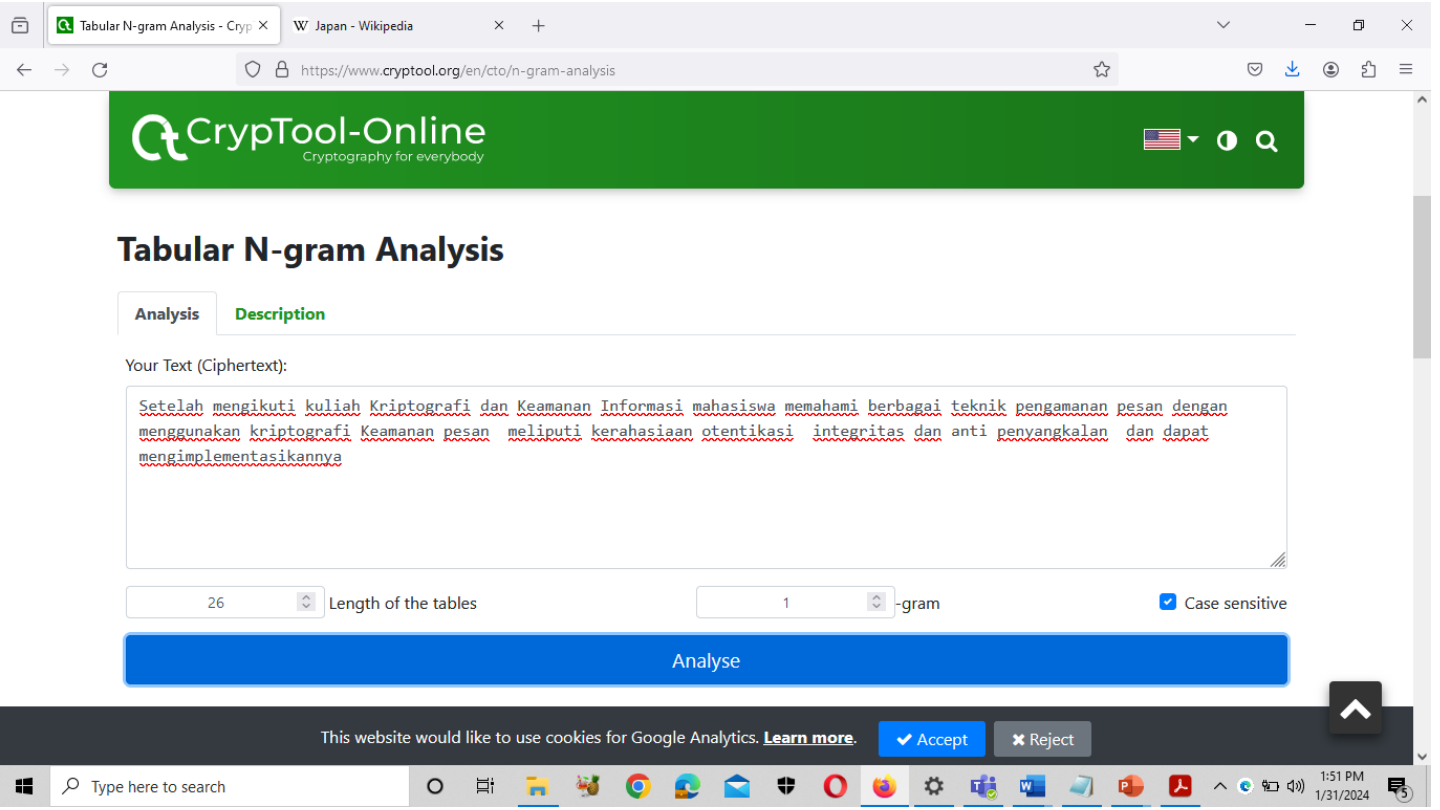
\includegraphics[width=157.50mm,height=222.75mm]{images/llm/page_011_img_01.png}%
\end{textblock*}

\newpage

% --- unit llm 12 ---
% === Halaman 12 (llm) ===

\vspace{164.54mm}

CrypTool-Online\newline Cryptography for everybody\newline\newline N-gram tables

% deskripsi: Tabel analisis N-gram yang menunjukkan peringkat (Rank), karakter 1-gram, jumlah absolut (Abs.), dan nilai relatif (Rel.) untuk sekumpulan karakter.
% bbox normalisasi: [0.1220, 0.3160, 0.4950, 0.8700]
\begin{textblock*}{78.33mm}(25.62mm,93.85mm)
\noindent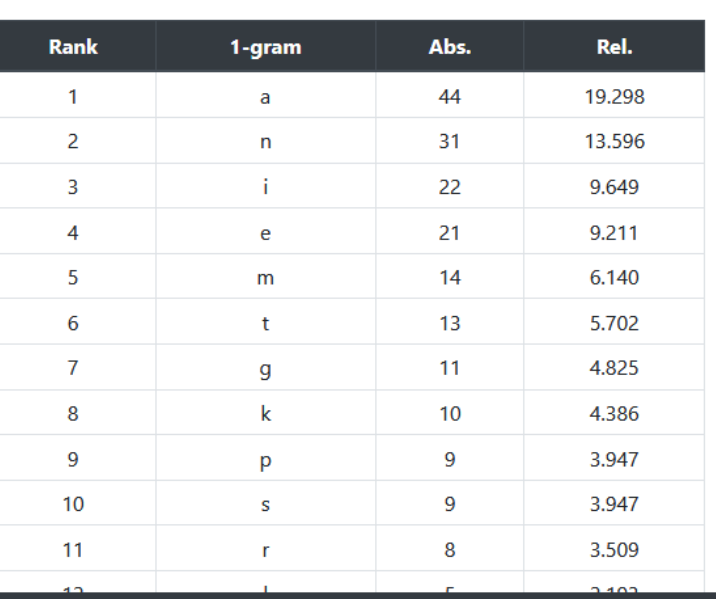
\includegraphics[width=78.33mm,height=164.54mm]{images/llm/page_012_img_01.png}%
\end{textblock*}

\newpage

% --- unit llm 13 ---
% === Halaman 13 (llm) ===

\textbf{Contoh 1:} Diberikan cipherteks berikut ini (Stalling, 2011), spasi tidak dibuang:

UZ QSO VUOHXMOPV GPOZPEVSG ZWSZ OPFPESX UDBMETSX AIZ
VUEPHZ HMDZSHZO WSFP APPD TSVP QUZW YMXUZUHSX
EPYEPOPDZSZUFPO MB ZWP FUPZ HMDJ UD TMOHMQ

\vspace{5mm}

Kita akan malakukan kriptanalisis dengan metode analisis frekuensi untuk memperoleh plainteks.

\vspace{5mm}

Asumsi: bahasa yang digunakan adalah Bahasa Inggris dan \textit{cipher} yang digunakan adalah \textit{cipher} abjad-tunggal.

\newpage

% --- unit llm 14 ---
% === Halaman 14 (llm) ===

\vspace{174.64mm}

Hitung frekuensi kemunculan huruf di dalam cipherteks tersebut sbb:\
\n\vspace{40mm}\

Jumlah total huruf, $N = 120$\n
\[ CI = \frac{\sum_{i=1}^{21} f_i(f_i-1)}{N(N-1)} = \frac{916}{120(119)} = 0,0641 \]

Nilai CI sangat dekat dengan 0,065 (teks bahasa Inggris), jauh dari 0,038 (teks acak/polyalphabetic cipher), maka kemungkinan besar ini adalah cipherteks dari \textit{monoalphabetic cipher}

% deskripsi: Dua tabel frekuensi kemunculan huruf (1-gram) yang mencakup peringkat (Rank), huruf (1-gram), jumlah absolut (Abs.), dan frekuensi relatif (Rel.)
% bbox normalisasi: [0.0480, 0.1320, 0.9520, 0.7200]
\begin{textblock*}{189.84mm}(10.08mm,39.20mm)
\noindent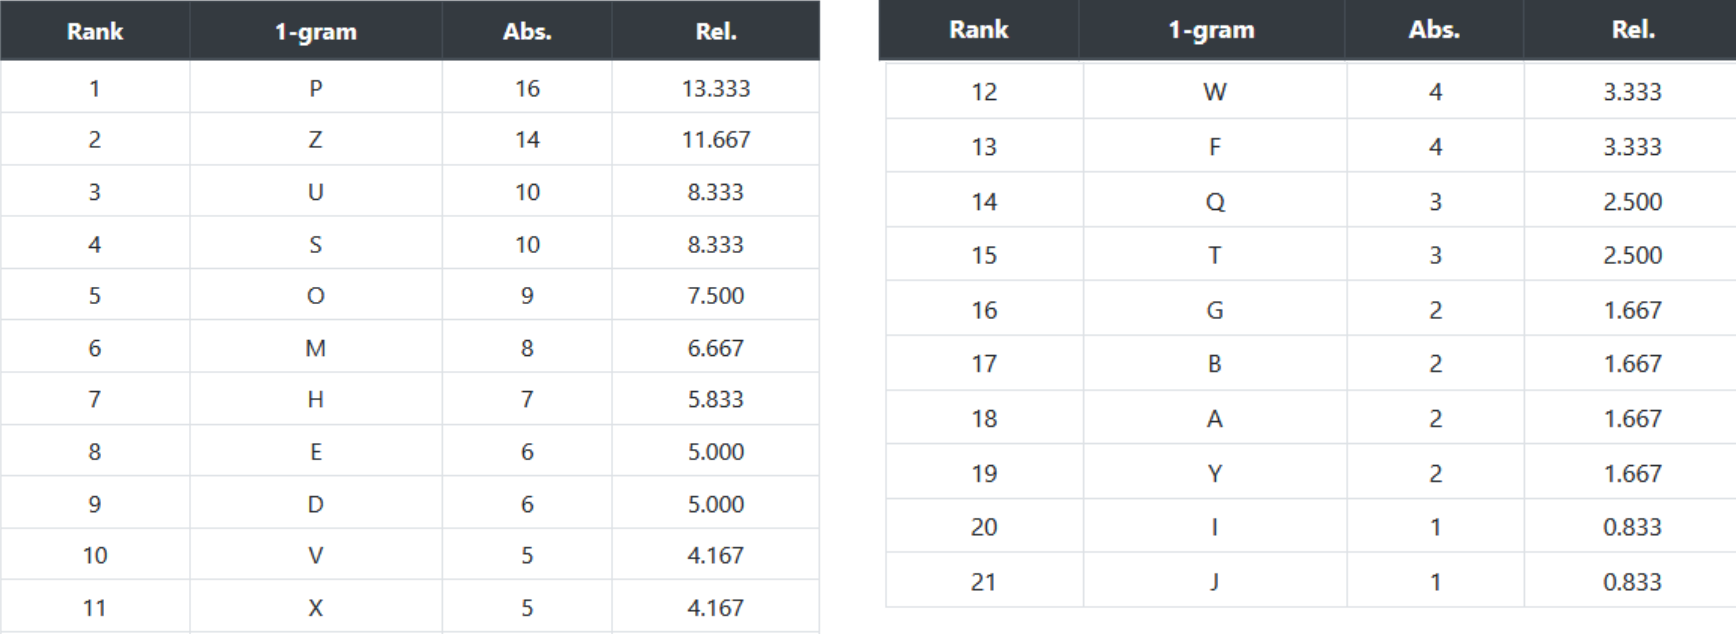
\includegraphics[width=189.84mm,height=174.64mm]{images/llm/page_014_img_01.png}%
\end{textblock*}

\newpage

% --- unit llm 15 ---
% === Halaman 15 (llm) ===

\vspace{172.26mm}

\vspace{10mm}
\begin{itemize}
    \item Dua huruf yang paling sering muncul di dalam cipherteks: huruf P dan Z.
    \item Dua huruf yang paling sering muncul di dalam B. Inggris: huruf E dan T.
    \item Kemungkinan besar,
    \begin{itemize}
        \item P adalah pemetaan dari e
        \item Z adalah pemetaan dari t
    \end{itemize}
    \item Tetapi kita belum dapat memastikannya sebab masih diperlukan cara \textit{trial and error} dan pengetahuan tentang Bahasa Inggris.
    \item Tetapi ini adalah langkah awal yang bagus.
\end{itemize}

% deskripsi: Tabel frekuensi kemunculan 1-gram yang menampilkan Rank, 1-gram, Absolut, dan Relatif.
% bbox normalisasi: [0.0280, 0.1800, 0.4300, 0.7600]
\begin{textblock*}{84.42mm}(5.88mm,53.46mm)
\noindent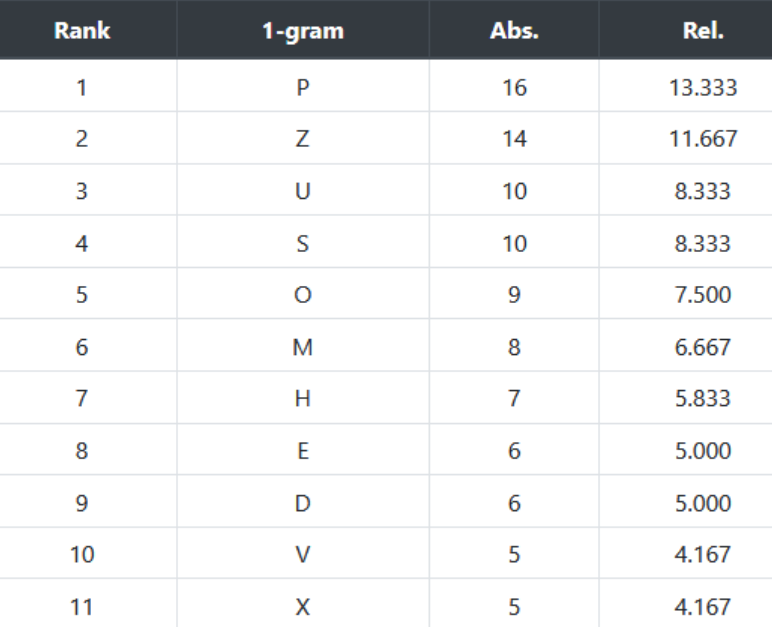
\includegraphics[width=84.42mm,height=172.26mm]{images/llm/page_015_img_01.png}%
\end{textblock*}

\newpage

% --- unit llm 16 ---
% === Halaman 16 (llm) ===

\section*{Iterasi 1:}

\vspace{10mm}

\begin{itemize}
    \item ZWP dan ZWSZ dipetakan menjadi $\text{t}*\text{e}$ dan $\text{t}**\text{t}$
    \item Kemungkinan besar $\text{W}$ adalah pemetaan dari $\text{H}$ sehingga kata yang mungkin untuk $\text{ZWP}$ dan $\text{ZWSZ}$ adalah $\text{the}$ dan $\text{that}$
\end{itemize}

% deskripsi: Kumpulan teks tersandi (ciphertext) dengan beberapa huruf yang sudah terpecahkan (plaintext) di bawahnya sebagai bagian dari proses kriptanalisis.
% bbox normalisasi: [0.1100, 0.1800, 0.7120, 0.5840]
\begin{textblock*}{126.42mm}(23.10mm,53.46mm)
\noindent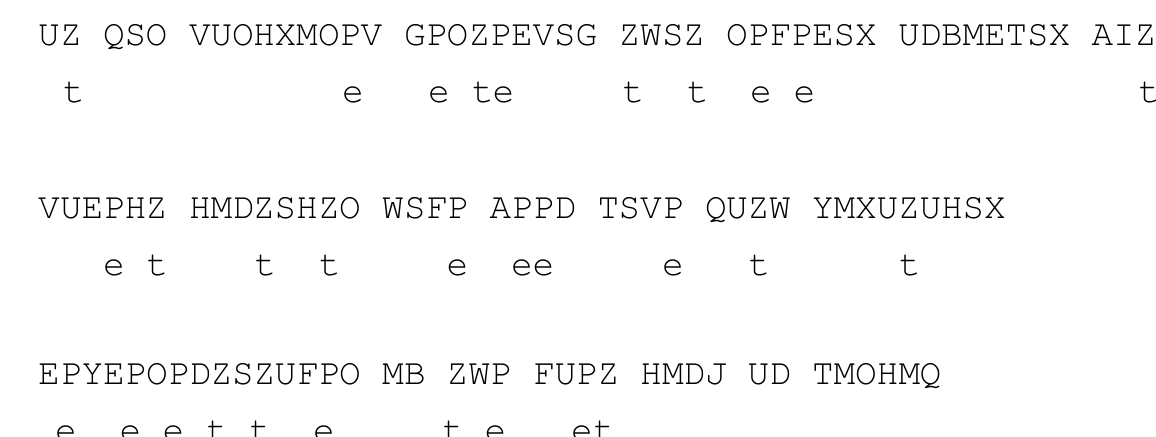
\includegraphics[width=126.42mm,height=119.99mm]{images/llm/page_016_img_01.png}%
\end{textblock*}

\newpage

% --- unit llm 17 ---
% === Halaman 17 (llm) ===

\begin{itemize}
    \item Diperoleh pemetaan (cipherteks $\rightarrow$ plainteks):
    \[
    \begin{aligned}
    P \rightarrow e \\ 
    Z \rightarrow t \\ 
    W \rightarrow h \\ 
    S \rightarrow a
    \end{aligned}
    \]
    \item Iterasi 2:
\end{itemize}

\vspace{5mm}

\begin{verbatim}
UZ QSO VUOHXMOPV GPOZPEVSG ZWSZ OPFPESX UDBMETSX AIZ
t a e e te a that e e a a t

VUEPHZ HMDZSHZO WSFP APPD TSVP QUZW YMXUZUHSX\ne t ta t ha e ee a e th t a

EPYEP OPDZSZUFPO MB ZWP FUPZ HMDJ UD TMOHMQ\ne e e tat e the et
\end{verbatim}

\newpage

% --- unit llm 18 ---
% === Halaman 18 (llm) ===

\begin{itemize}
    \item $\text{WSFP}$ dipetakan menjadi $\text{ha*e}$.
    \item Dalam Bahasa Inggris, kata yang mungkin untuk $\text{ha*e}$ hanyalah $\text{ha\textcolor{red}{v}e}$, $\text{ha\textcolor{red}{t}e}$, $\text{ha\textcolor{red}{l}e}$, dan $\text{ha\textcolor{red}{z}e}$.
    \item Dengan mencoba mengganti semua $\text{F}$ di dalam cipherteks dengan $\text{v, t, l,}$ dan $\text{z}$, maka huruf yang cocok adalah $\text{v}$ sehingga $\text{WSFP}$ dipetakan menjadi $\text{have}$.
    \item Dengan mengganti $\text{F}$ menjadi $\text{v}$ pada kriptogram $\text{EPYEPOPDZSZUFPO}$ sehingga menjadi $\text{*e*e*e*tat*ve*}$, maka kata yang cocok untuk ini adalah $\text{representatives}$.
\end{itemize}

\newpage

% --- unit llm 19 ---
% === Halaman 19 (llm) ===

\begin{itemize}
    \item Diperoleh pemetaan:
    \[ 
    \begin{aligned}
    E \rightarrow r && Y \rightarrow p \\
    U \rightarrow I && O \rightarrow s \\
    D \rightarrow n && 
    \end{aligned}
    \]
    \vspace{5mm}
    \item Hasil akhir bila diselesaikan seluruhnya:
    \begin{verbatim}
    It was disclosed yesterday that several informal but
    direct contacts have been made with political
    representatives of the viet cong in Moscow
    \end{verbatim}
    \vspace{5mm}
    \item Tabel substitusi yang dihasilkan:
    \begin{verbatim}
    Plainteks:  A B C D E F G H I J K L M N O P Q R S T U V W X Y Z
    Cipherteks: S A H V P B J W U - - X T D M Y Z E O Z I F Q - G -
    \end{verbatim}
\end{itemize}

\newpage

% --- unit llm 20 ---
% === Halaman 20 (llm) ===

\textbf{Contoh 2:} Diberikan cipherteks berikut ini, yang dihasilkan dari cipher abjad-Tunggal. Lakukan dekripsi untuk mengungkap plainteksnya.\\
\nLIVITCSWPIYVEWHEVSRIQMXLEYVEOIEWHRXEXIPFEMVEWHKVSTYLXZIX\nLIKI IXPIJVSZEYPERRGERIMWQLMGLMXQERIWGPSRIHMXQEREKIETXMJT\nPRGEVEKEITREWHEXXLEXXMZITWAWSQWXSWEXTVEPMRXRSJGSTVRIEYVI\nEXCVUMIWERGMIWXMJMGCSMWXSW JQMIXQLIVIQIVIXQSVSTWHKPEGARCS\nXRWIEWSWIIBXVIZMXFSJXLIKEGAEWHEPSWYSWIWIEVXLISXLIVLX LIRGE\nPIRQIVIIBGIIHMWYPFLEVHEWHYPSRR FQMXLEPPXLIECCIEVEWGISJKTV\nWMRLIHYSPHXLIQIMYLX SJXLIMWRIGXQEROIVFVIZEV AEKPIEWHXEAMWY\nEPPXLMWY RMWX XGSWRMHIVEXMSWMGSTPHLEVH PFKPE ZINTCMXIVJ SVLMR\nSCMWM SWVIRCIGXMWYMX

\newpage

% --- unit llm 21 ---
% === Halaman 21 (llm) ===

\begin{itemize}
  \item Hasil perhitungan frekuensi kemunculan huruf, bigram, dan trigram:
  \begin{itemize}
    \item huruf I paling sering muncul,
    \item XL adalah bigram yang paling sering muncul,
    \item XLI adalah trigram yang paling sering muncul.
  \end{itemize}
\end{itemize}

Ketiga data terbanyak ini menghasilkan dugaan bahwa

\begin{align*}
  \text{I} & \text{ berkoresponden dengan huruf plainteks e,}\
  \text{XLI} & \text{ berkoresponden dengan the,}\
  \text{XL} & \text{ berkoresponden dengan th}
\end{align*}

Pemetaan:

\begin{align*}
  \text{I} & \rightarrow \text{e}\
  \text{X} & \rightarrow \text{t}\
  \text{L} & \rightarrow \text{h}
\end{align*}

\newpage

% --- unit llm 22 ---
% === Halaman 22 (llm) ===

\begin{itemize}
    \item \texttt{XLEX} dipetakan menjadi \texttt{th*t}.
    \item Kata yang cocok untuk \texttt{th*t} adalah \texttt{that}.
    \item Jadi kita memperoleh: $\text{E} \rightarrow \text{a}$
    \item Hasil iterasi pertama:
\end{itemize}

\vspace{5mm}

\begin{center}
\texttt{heVeTCSWPeYVaWHaVSReQMthaYVaOeaWHRtatePFaMVaWHKVSTYhtZe\\
theKeetPeJVSZaYPaRRGaReMWQhMGHtQaReWGPSReHMtQaRaKeaTtM\\
JTPRGaVaKaeTRaWHattattMZeTWAWSQWtSwatTVaPMRtRSJGSTVRea\\
YVeatCVMUeMWarGMeWtMJMGCSMWtSJOmeQtheVeQeVetQSVSTWHKPaG\\
ARCStRWeaVSWeeBtVeZMtFSJtheKGaAAWhaPSWYSWeWeaVtheStheVt\\
heRGaPeRQeVeeBGeeHMWYPFhaVHAWHYPSR RFQMthaPPtheaCCeaVaWG\\
eSJKTVWMRheHYSPHtheQeMYhtSJtheMWReGtQaROeVFeZaVAaKPeaW\\
HtaAMWYaPPthMWYRMWtSGSWRMHeVatMSWMGSTPHhaVHPFKPaZeNTCMt\\
eVJSVhMRSCMWMSWVeRCeGtMWYyMt}
\end{center}

\newpage

% --- unit llm 23 ---
% === Halaman 23 (llm) ===

\begin{itemize}
    \item Selanjutnya,
    \begin{itemize}
        \item \texttt{Rtate} mungkin adalah \texttt{state},
        \item \texttt{atthattMZE} mungkin adalah \texttt{atthattime},
        \item \texttt{heVe} mungkin adalah \texttt{here}.
    \end{itemize}
    \item Jadi, kita memperoleh pemetaan baru:
    \[
    \begin{aligned}
    R & \rightarrow s \\
    M & \rightarrow i \\
    Z & \rightarrow m \\
    V & \rightarrow r
    \end{aligned}
    \]
\end{itemize}

\newpage

% --- unit llm 24 ---
% === Halaman 24 (llm) ===

\begin{itemize}
  \item Hasil iterasi ke-2:
\end{itemize}

\vspace{5mm}

\begin{flushleft}
hereTCSWPeYraWHarSseQithaYraOeaWHstatePFairaWHKrSTYhtm\\
etheKeetPeJrSmaYPassGaseiWQhiGhitQaseWGPSseHitQasaKeaT\\
tiJTPsGaraKaeTsaWHThatthattimeTWAWSQWtSwatTraPistsSJGSTr\\
seaYreatCriUeiWasGieWtiJiGCSiWtSJioeQthereQeretQsRSTWH\\
KPaGAsCStsWearSWeeBtremitFSJtheKaGaaWHaPSWYSWeWeartheS\\
therthesGaPesQereeBGeeHiWYPFharHaWHYPSssFQithaPPtheaCC\\
earaWGeSJKTrWisheHYSPHtheQeiYhtSJtheiWseGtQasOerFremar\\
AaKPeaWHtaAiWYaPPthiWYsiWtSGSWsiHeratiSWIGSTPHharHPFKP\\
ameNTCiterJSrhisSCiWiSWresCeGtiWYit
\end{flushleft}

\vspace{10mm}

\begin{itemize}
  \item Teruskan, dengan menerka kata-kata yang sudah dikenal, misalnya\\
  \quad remarA mungkin \textit{remark}, dsb
\end{itemize}

\newpage

% --- unit llm 25 ---
% === Halaman 25 (llm) ===

\begin{itemize}
  \item Hasil iterasi 3:
\end{itemize}

\noindent hereuponlegrandarosewithagraveandstatelyairandbr\newline oughtmethebeetlefromaglasscaseinwhichitwasenclos\newline editwasabeautifulscarabaeusandatthattimeunknown t\newline onaturalistsofcourseagreatprizeinascientificpoin\newline tofviewthereweretworoundblackspotsnearoneextremi\newline tyofthebackandalongoneneartheotherthescalesweree\newline xceedinglyhardandglossywithalltheappearanceofbur\newline nishedgoldtheweightoftheinsectwasveryremarkablea\newline ndtakingallthingsintoconsiderationicouldhardlybl\newline amejupiterfor*hisopininionrespectingit

\newpage

% --- unit llm 26 ---
% === Halaman 26 (llm) ===

\begin{itemize}
  \item Tambahkan spasi, tanda baca, dll
\end{itemize}

Here upon Legrand arose, with a grave and stately air, and brought me the beetle from a glass case in which it was enclosed. It was a beautiful scarabaeus, and, at that time, unknown to naturalists--of course a great prize in a scientific point of view. There were two round black spots near one extremity of the back, and a long one near the other. The scales were exceedingly hard and glossy, with all the appearance of burnished gold. The weight of the insect was very remarkable, and, taking all things into consideration, I could hardly blame Jupiter for his opinion respecting it.

\newpage

% --- unit llm 27 ---
% === Halaman 27 (llm) ===

\section*{B. Vig\`enere Cipher}

\begin{itemize}
    \item Vigenere Cipher termasuk ke dalam kelompok \textit{cipher} abjad-majemuk (\textit{polyalphabetic cipher}). Ini berbeda dengan cipher abjad-tunggal (\textit{monolphabetic cipher}).
    \item Perbedaan \textit{polyalphabetic cipher} dengan \textit{monoalphabetic cipher}:
    \begin{itemize}
        \item[$\blacktriangleright$] \textit{Cipher} abjad-tunggal: satu kunci untuk semua huruf plainteks \\ Contoh: Caesar cipher
        \item[$\blacktriangleright$] \textit{Cipher} abjad-majemuk: setiap huruf menggunakan kunci berbeda. \\ Contoh: Vigenere cipher
    \end{itemize}
    \item \textit{Cipher} abjad-majemuk dibuat untuk mengatasi kelemahan \textit{cipher} abjad-Tunggal yang mudah dipecahkan dengan teknik analisis frekuensi
\end{itemize}

\newpage

% --- unit llm 28 ---
% === Halaman 28 (llm) ===

\section*{Bentuk umum \textit{cipher} abjad-majemuk}

\begin{itemize}
    \item Kunci:
    \[ K = k_1 k_2 \dots k_m \quad \text{(ket: } m = \text{ panjang kunci)} \]
    Karena $m$ lebih pendek daripada panjang plainteks, maka kunci diulang secara periodik
    
    \item Plainteks:
    \[ P = p_1 p_2 \dots p_m p_{m+1} \dots p_{2m} \dots \]
    
    \item Cipherteks:
    \[ C = E_k(P) = f_{k_1}(p_1) f_{k_2}(p_2) \dots f_{k_m}(p_m) f_{k_1}(p_{m+1}) f_{k_2}(p_{m+2}) \dots f_{k_m}(p_{2m}) \dots \]
    $f(.)$ adalah fungsi enkripsi pada \textit{cipher} abjad-tunggal

    \item Untuk $m = 1$, \textit{cipher}-nya ekivalen dengan \textit{cipher} abjad-tunggal.
\end{itemize}

\newpage

% --- unit llm 29 ---
% === Halaman 29 (llm) ===

\begin{itemize}
    \item Misalkan panjang kunci $m = 10$, maka 10 huruf pertama plainteks dienkripsi dengan kunci $K$, setiap huruf ke-$i$ menggunakan kunci $k_i$.
    \item Untuk 10 karakter berikutnya, kembali menggunakan pola enkripsi yang sama.
\end{itemize}

\noindent Contoh: kunci = \texttt{sony} \quad ($m = 4$)\
Plainteks: \texttt{thisplaintexthissecret}\
Kunci: \texttt{sonysonysonysonysonys}

\vspace{5mm}

Setiap huruf plainteks dienkripsi dengan huruf kunci di bawahnya dengan \textit{cipher} abjad tunggal (misalnya menggunakan \textit{Caesar Cipher}):

\begin{align*}
    (t+s) \pmod{26} \\
    (h + o) \pmod{26} \\
    (i + n) \pmod{26} \\
    \text{dst...}
\end{align*}

\newpage

% --- unit llm 30 ---
% === Halaman 30 (llm) ===

\vspace{95.04mm}

\section*{Sejarah Vigenere Cipher}

\begin{itemize}
    \item Penemu \textit{cipher} ini sebenarnya adalah Giovan Batista Belaso, karena ia menggambarkan pertama kali pada tahun 1553 seperti ditulis di dalam bukunya \textit{La Cifra del Sig. Giovan Batista Belaso}.
    \item Namun, \textit{cipher} ini disempurnakan dan dipublikasikan oleh diplomat (sekaligus seorang kriptologis) Perancis, Blaise de Vig\grave{e}nere pada abad 16 (tahun 1586).
    \item Pada abat ke-19, banyak orang yang mengira Vigen\grave{e}re adalah penemu \textit{cipher} ini, sehingga dikenal luas sebagai \textit{Vigen\grave{e}re Cipher}.
\end{itemize}

% deskripsi: Potret Blaise de Vigenère
% bbox normalisasi: [0.8370, 0.0050, 0.9720, 0.3250]
\begin{textblock*}{28.35mm}(175.77mm,1.49mm)
\noindent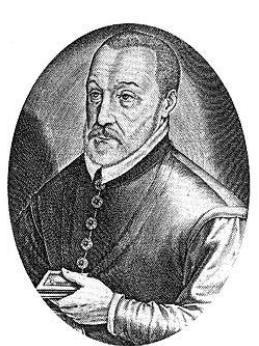
\includegraphics[width=28.35mm,height=95.04mm]{images/llm/page_030_img_01.png}%
\end{textblock*}

\newpage

% --- unit llm 31 ---
% === Halaman 31 (llm) ===

\section*{Blaise de Vigen\`ere}

\textbf{Blaise de Vigen\`ere} (French: [\text{vi\textsubscript{z}\textepsilon\textsubscript{r} \textepsilon}]; 5 April 1523 -- 19 February 1596)$^{[1]}$ was a French diplomat, cryptographer, translator and alchemist.

\vspace{205.23mm}

\subsection*{Biography [ edit ]}

Vigen\`ere was born into a respectable family in the village of Saint-Pour\c{c}ain in Bourbonnais. When he was 12, his father, Jehan (modern spelling Jean) de Vigen\`ere, arranged for him to have a classical education in Paris. Registered at the university at 14, he quit after three years without a known degree.$^{[2]}$

\vspace{10mm}

From 1539 to around 1545, he worked under Gilbert Bayard, a first secretary to King Francis I, who had fiefs in Bourbonnais.$^{[2]}$

In 1545, he accompanied the French envoy Louis Adh{\'e}mar de Monteil, Count of Grignan, to the Diet of Worms as a junior secretary.$^{[3][4]}$ After the diet's rupture, he traveled in Europe.$^{[5]}$

In 1547, he quit the court and entered the service of the House of Nevers. He would remain associated with it until at least a year before

Sumber: Wikipedia

% deskripsi: Infobox Wikipedia tentang Blaise de Vigenère yang berisi potret wajah dan rincian biografi seperti tanggal lahir, tanggal wafat, pekerjaan, dan hal yang dikenal.
% bbox normalisasi: [0.5660, 0.2220, 0.7840, 0.9130]
\begin{textblock*}{45.78mm}(118.86mm,65.93mm)
\noindent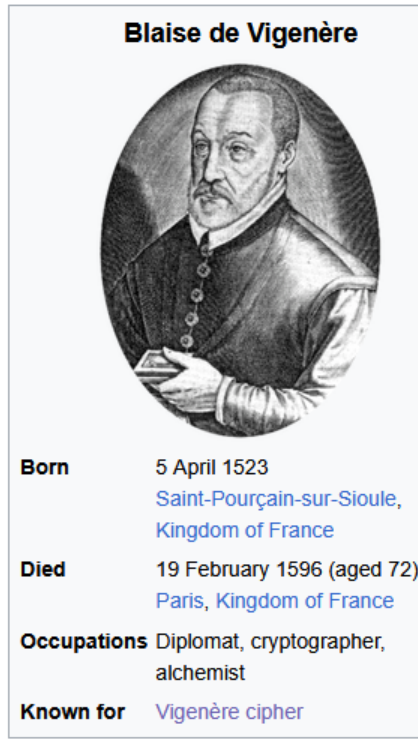
\includegraphics[width=45.78mm,height=205.23mm]{images/llm/page_031_img_01.png}%
\end{textblock*}

\newpage

% --- unit llm 32 ---
% === Halaman 32 (llm) ===

\begin{itemize}
  \item \textit{Cipher} ini berhasil dipecahkan oleh Babbage dan Kasiski pada pertengahan Abad 19 (akan dijelaskan pada materi selanjutnya).
  \item Kasiski menguraikan langkah-Langkah untuk menemukan panjang kunci (bukan huruf-huruf kunci kunci ).
  \item \textit{Vig\grave{e}nere Cipher} digunakan oleh Tentara Konfederasi (\textit{Confederate Army}) pada Perang Sipil Amerika (\textit{American Civil war}).
  \item Perang Sipil terjadi setelah \textit{Vig\grave{e}nere Cipher} berhasil dipecahkan.
\end{itemize}

\newpage

% --- unit llm 33 ---
% === Halaman 33 (llm) ===

\vspace{259.88mm}

\begin{itemize}
    \item \textit{Vig\grave{e}n\grave{e}re Cipher} menggunakan tabel Vig\grave{e}n\grave{e}re -- dinamakan Vig\grave{e}n\grave{e}re square, untuk melakukan enkripsi dan dekripsi.
    \item Setiap baris $i$ di dalam bujursangkar menyatakan huruf-huruf cipherteks yang diperoleh menggunakan \textit{Caesar Cipher} dengan kunci $k = i$.
    \item Artinya, setiap baris $i$ merupakan pergeseran huruf alfabet sejauh $i$ ke kanan
\end{itemize}

% deskripsi: Tabel Vigenere square yang menunjukkan pergeseran alfabet untuk enkripsi dan dekripsi
% bbox normalisasi: [0.4240, 0.0570, 0.9820, 0.9320]
\begin{textblock*}{117.18mm}(89.04mm,16.93mm)
\noindent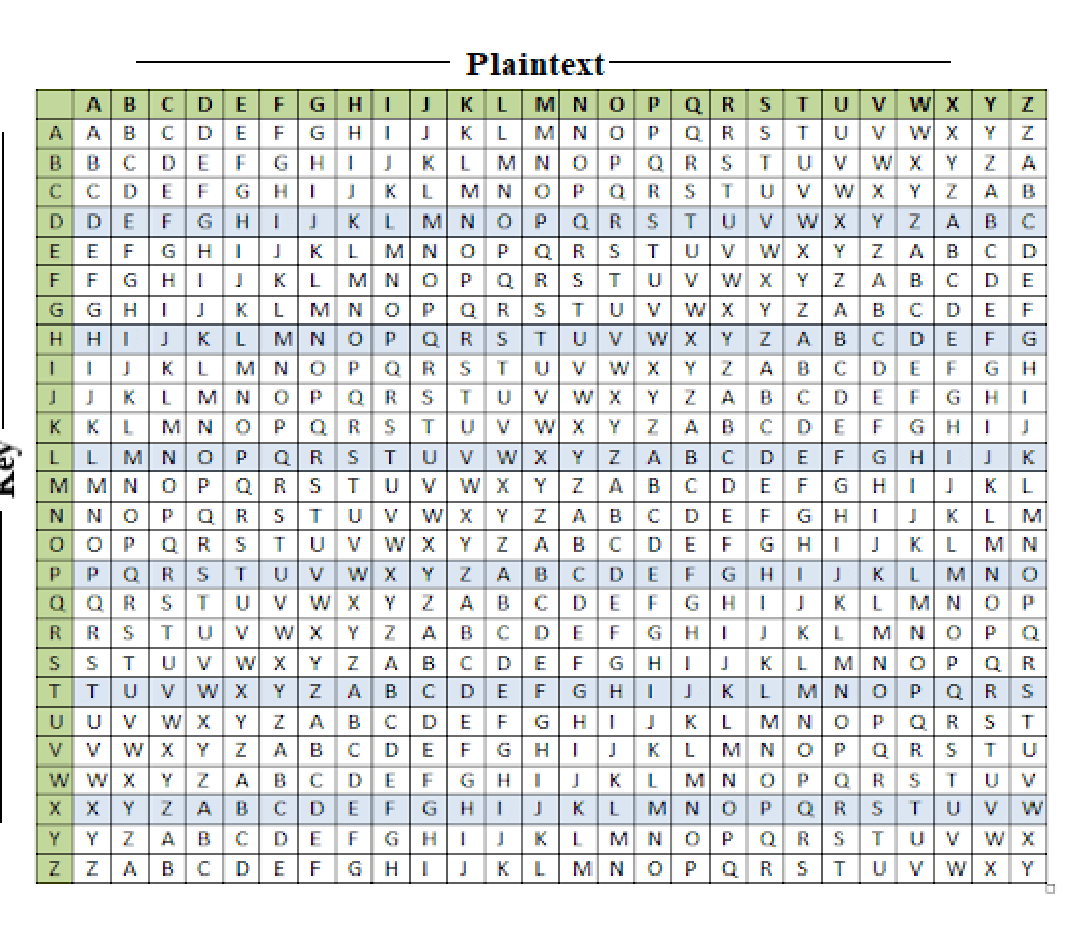
\includegraphics[width=117.18mm,height=259.88mm]{images/llm/page_033_img_01.png}%
\end{textblock*}

\newpage

% --- unit llm 34 ---
% === Halaman 34 (llm) ===

\vspace{228.69mm}

\begin{center}
\vspace{10mm}
\end{center}

% deskripsi: Ilustrasi tabel Vigenère atau Caesar cipher shift yang menunjukkan pergeseran alfabet untuk enkripsi, dengan label 'Plaintext' di atas dan 'Key' di samping, serta keterangan 'baris ke-0' dan 'baris ke-25'.
% bbox normalisasi: [0.1300, 0.1000, 0.7600, 0.8700]
\begin{textblock*}{132.30mm}(27.30mm,29.70mm)
\noindent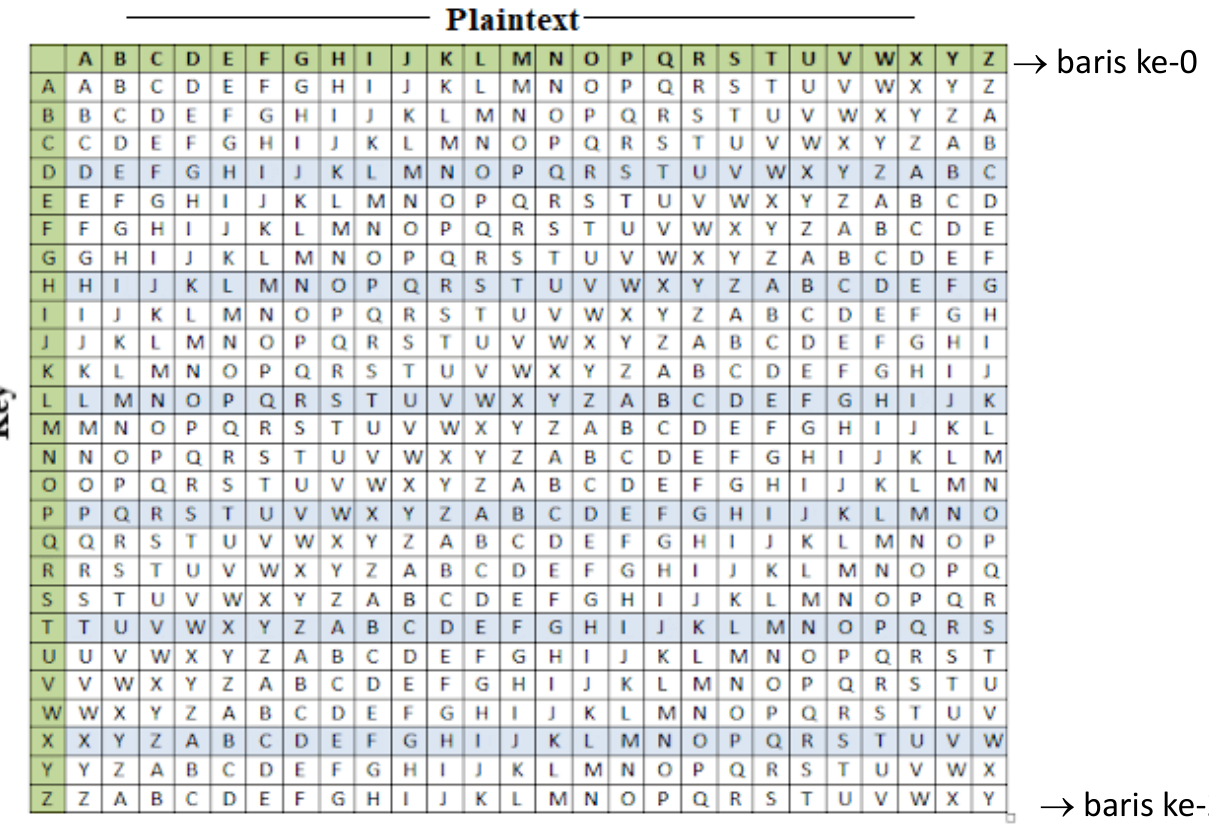
\includegraphics[width=132.30mm,height=228.69mm]{images/llm/page_034_img_01.png}%
\end{textblock*}

\newpage

% --- unit llm 35 ---
% === Halaman 35 (llm) ===

\vspace{44.55mm}

\begin{itemize}
    \item Kunci adalah string: $K = k_1 k_2 \dots k_m$
    $k_i$ untuk $1 \le i \le m$ menyatakan huruf-huruf alfabet
    
    \item Jika panjang kunci lebih pendek daripada panjang plainteks, maka kunci diulang secara periodik.
    
    \item Misalkan panjang kunci $m = 10$, maka 10 huruf pertama plainteks dienkripsi dengan kunci $K$, setiap huruf ke-$i$ menggunakan kunci $k_i$.
\end{itemize}

\vspace{10mm}

Contoh: kunci = \texttt{soreang} \quad (dalam angka: $18, 14, 17, 4, 0, 13, 6$)

\begin{tabular}{ll}
Plainteks: & \texttt{terimapesanangulaikambing} \\
Kunci: & \texttt{soreangsoreangsoreangsore}
\end{tabular}

\vspace{5mm}

Untuk 8 karakter berikutnya, kembali menggunakan pola enkripsi yang sama.

% deskripsi: Tabel pemetaan huruf alfabet ke angka dari A=0 sampai Z=25
% bbox normalisasi: [0.5300, 0.0000, 0.9800, 0.1500]
\begin{textblock*}{94.50mm}(111.30mm,0.00mm)
\noindent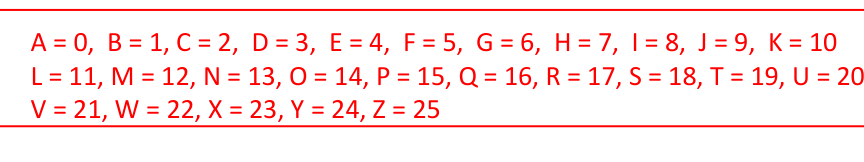
\includegraphics[width=94.50mm,height=44.55mm]{images/llm/page_035_img_01.png}%
\end{textblock*}

% deskripsi: Kotak penjelasan yang menyatakan bahwa setiap huruf plainteks dienkripsi menggunakan Caesar Cipher dengan kunci k yang berbeda-beda
% bbox normalisasi: [0.6300, 0.6700, 0.9800, 0.8100]
\begin{textblock*}{73.50mm}(132.30mm,198.99mm)
\noindent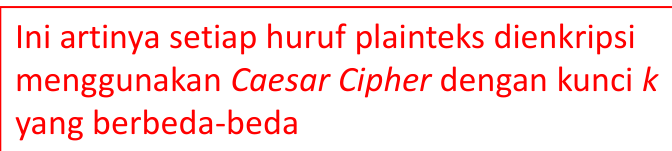
\includegraphics[width=73.50mm,height=41.58mm]{images/llm/page_035_img_02.png}%
\end{textblock*}

\newpage

% --- unit llm 36 ---
% === Halaman 36 (llm) ===

\bullet Enkripsi dilakukan dengan mencari titik potong huruf plainteks dengan huruf kunci:

\vspace{10mm}

\begin{flushright}
\begin{tabular}{lll}
Plainteks & : & \textcolor{red}{terimapesanangulaikambing} \\
Kunci & : & \textcolor{red}{soreangsoreangsoreangsore} \\
Cipherteks & : & \textcolor{red}{LSimMNVWGRRAAMMZRMKNSTWEK} \\
\end{tabular}
\end{flushright}

\vspace{120mm}

Gambar 4.3 Enkripsi huruf $\mathcal{T}$ dengan kunci $\mathcal{S}$

% deskripsi: Tabel Vigenere Square yang menunjukkan pemetaan huruf untuk enkripsi cipher
% bbox normalisasi: [0.0000, 0.2150, 0.7500, 0.9300]
\begin{textblock*}{157.50mm}(0.00mm,63.85mm)
\noindent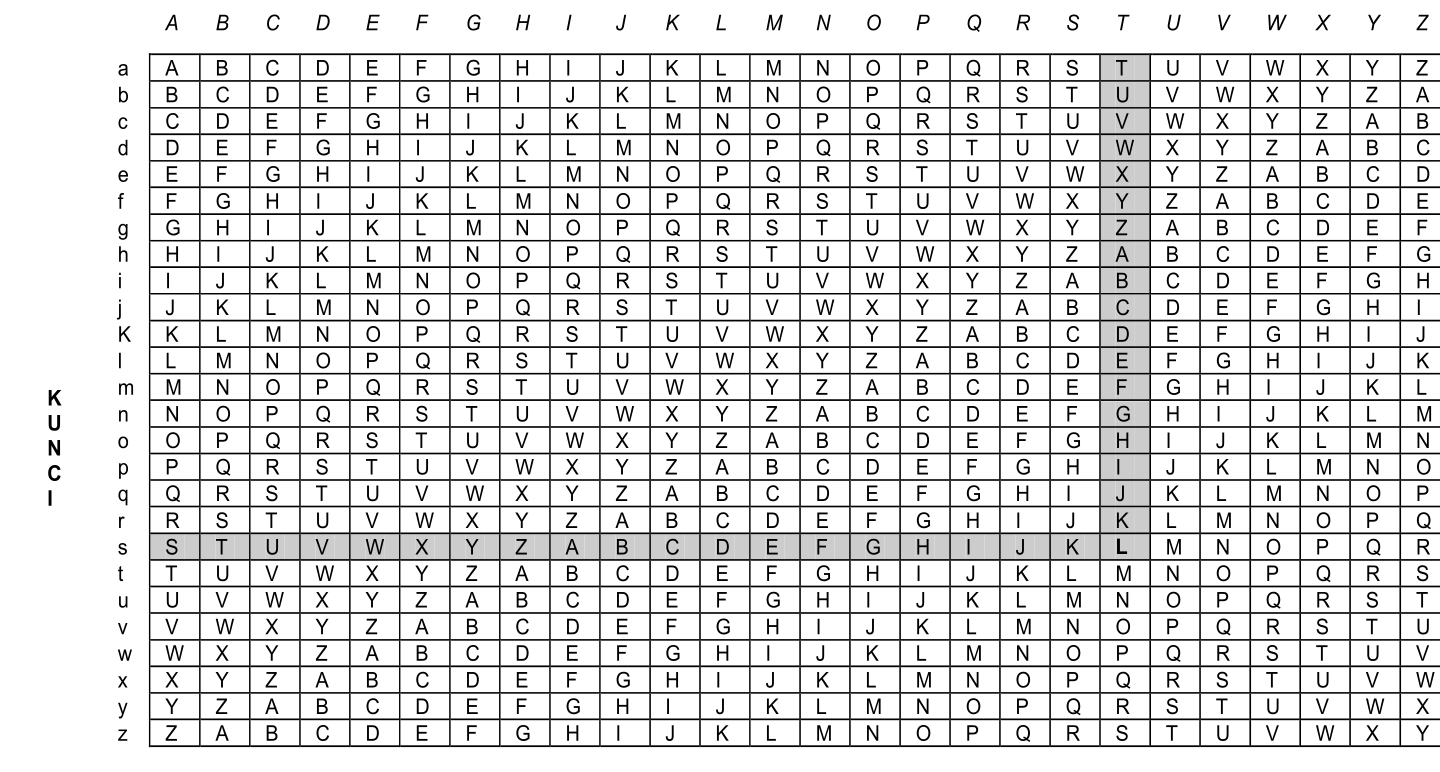
\includegraphics[width=157.50mm,height=212.36mm]{images/llm/page_036_img_01.png}%
\end{textblock*}

\newpage

% --- unit llm 37 ---
% === Halaman 37 (llm) ===

\vspace{32.08mm}

\begin{itemize}
    \item Hasil enkripsi seluruhnya adalah sebagai berikut:

    \begin{tabular}{ll}
        Plainteks & : terimapesanangulaikambing \\
        Kunci & : soreangsoreangsoreangsore \\
        Cipherteks & : LSIMMNVWGRRAAMMZRMKNSTWEK
    \end{tabular}

    \item Tanpa menggunakan \textit{Vigenere Square} pun enkripsi tetap dapat dihitung secara \textit{Caesar Cipher} dengan menjumlahkan plainteks $p_j$ dengan kunci $k_i$ dalam modulus 26:

    \begin{align*}
        \text{Enkripsi: } & c_j = E(p_j) = (p_j + k_i) \pmod{26} \tag{1} \\
        \text{Dekripsi: } & p_j = D(c_j) = (c_j - k_i) \pmod{26} \tag{2}
    \end{align*}

    Contoh:
    \[ (t + s) \pmod{26} = (19 + 18) \pmod{26} = 37 \pmod{26} = 11 = L \]
    \[ (e + o) \pmod{26} = (4 + 14) \pmod{26} = 18 \pmod{26} = 18 = S, \text{ dst} \]
\end{itemize}

% deskripsi: Kotak referensi pemetaan huruf alfabet ke angka dari A=0 sampai Z=25
% bbox normalisasi: [0.5320, 0.0080, 0.9860, 0.1160]
\begin{textblock*}{95.34mm}(111.72mm,2.38mm)
\noindent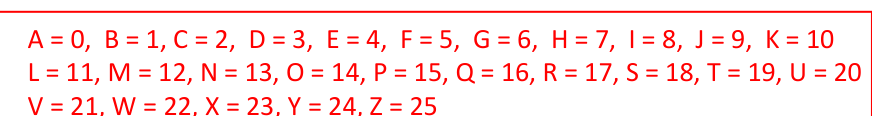
\includegraphics[width=95.34mm,height=32.08mm]{images/llm/page_037_img_01.png}%
\end{textblock*}

\newpage

% --- unit llm 38 ---
% === Halaman 38 (llm) ===

\begin{itemize}
    \item Kelebihan Vigenere Cipher: huruf plainteks yang sama tidak selalu dienkripsi menjadi huruf ciphteks yang sama pula, bergantung huruf kunci yang digunakan.

    Contoh: pada contoh di atas, huruf plainteks $\mathbb{T}$ dapat dienkripsi menjadi $\mathbb{L}$ atau $\mathbb{H}$, dan huruf cipherteks $\mathbb{V}$ dapat merepresentasikan huruf plainteks $\mathbb{H}$, $\mathbb{I}$, dan $\mathbb{X}$

    \item Hal di atas merupakan karakteristik dari \textit{cipher} abjad-majemuk: setiap huruf cipherteks dapat memiliki kemungkinan banyak huruf plainteks.

    \item Bandingkan dengan \textit{cipher} abjad-tunggal, setiap huruf cipherteks selalu menggantikan huruf plainteks tertentu.
\end{itemize}

\newpage

% --- unit llm 39 ---
% === Halaman 39 (llm) ===

\begin{itemize}
    \item Dengan karakteristik seperti terebut, maka distribusi kemunculan huruf di dalam cipherteks relatif mendekati seragam (\textit{uniform}) dan histogramnya cenderung \textit{flat} (datar)
    \item Histogram yang flat akan menyulitkan kriptanalisis memecahkan cipherteks dengan metode analisis frekuensi
\end{itemize}

\vspace{20mm}

% deskripsi: Perbandingan antara histogram yang flat (datar) dan histogram yang bukan flat, menunjukkan distribusi frekuensi huruf A sampai Z.
% bbox normalisasi: [0.1100, 0.4500, 0.8600, 0.9100]
\begin{textblock*}{157.50mm}(23.10mm,133.65mm)
\noindent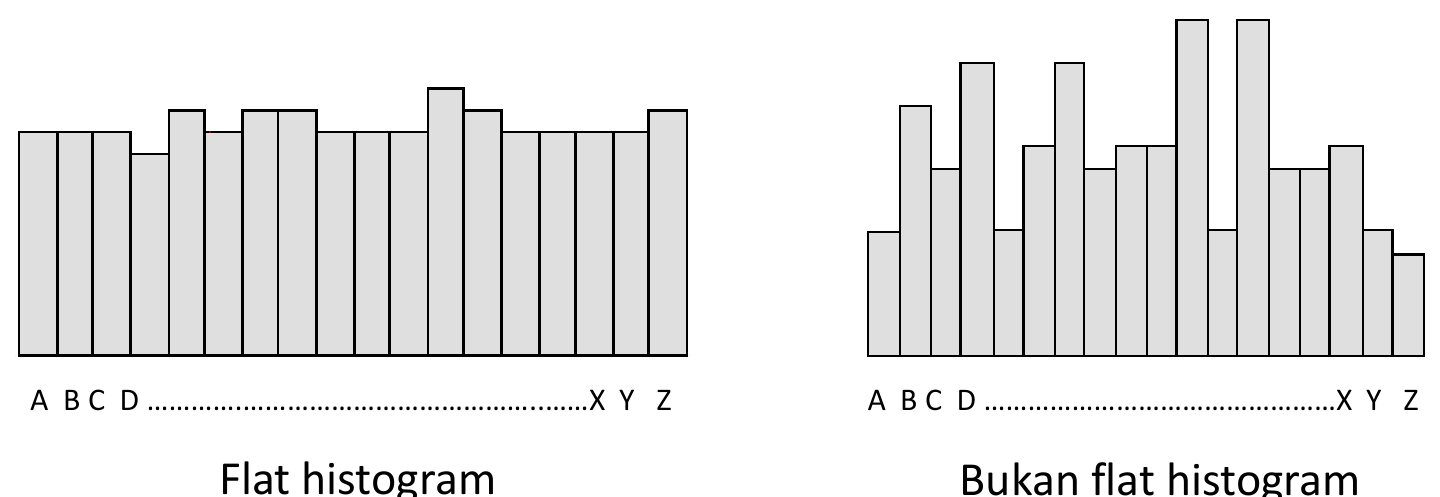
\includegraphics[width=157.50mm,height=136.62mm]{images/llm/page_039_img_01.png}%
\end{textblock*}

\newpage

% --- unit llm 40 ---
% === Halaman 40 (llm) ===

\textcolor{red}{Plainteks:} \begin{minipage}{0.75\textwidth}
Dinas Pendidikan Kota Ternate meminta kepada pihak sekolah dan orang tua siswa untuk jenjang pendidikan SD dan SMP se-Kota Ternate untuk melarang para siswa membawa permainan lato-lato yang sedang tren itu ke sekolah, karena akan mengganggu kegiatan belajar mengajar yang dinilai berbahaya sehingga mengantisipasi kecelakaan bagi anak di daerah itu.
\end{minipage}

\vspace{5mm}

\textcolor{red}{Kunci:} \textcolor{red}{selatsunda}

\vspace{5mm}

\textcolor{red}{Cipherteks:}
\textcolor{blue}{(dikelompokkan 4-huruf)} \begin{minipage}{0.75\textwidth}
VMYAL HYGAI VMVAG CIGDT WVYAM WGRPX FXLKX HUQDP ALLKL WEBOA
ZHLNH JUAJT MEDIL OUHQT MOUEG BUAJP WROIW AENQS VHLNL EJFHK
GXLTX JHNWE MREUD EYRDR SRRPT JUFLS OEXEF TUJDP WVXAB FUAOA
LSWAM GSNQG KIOAG YNEHN AXFKX KYXRL SLVAK WHNDK SRXEG YANQG
YYVEZ AUGDN TIWAC SLZHN YEUAK QUAJD ARTLT AVRUB SLLYT KYULN YKLMX
FANQT AWTPT KCXHC WPLKT SHODG AEYAD VCQDE JESIM M
\end{minipage}

\newpage

% --- unit llm 41 ---
% === Halaman 41 (llm) ===

\vspace{240.57mm}

\begin{itemize}
  \item Demo Vigenere Cipher online: \url{https://cryptii.com/pipes/vigenere-cipher}
\end{itemize}
\vspace{10mm}

% deskripsi: Screenshot antarmuka web Cryptii yang menunjukkan proses enkripsi teks menggunakan Vigenère cipher, dengan plaintext 'Betapa ramainya acara pertandingan sepakbola di lapangan itu Inginku ke sana, apadaya tidak punya karcis' dan kunci 'tabahkanhatimu', menghasilkan ciphertext yang terenkripsi.
% bbox normalisasi: [0.0600, 0.1300, 0.9300, 0.9400]
\begin{textblock*}{182.70mm}(12.60mm,38.61mm)
\noindent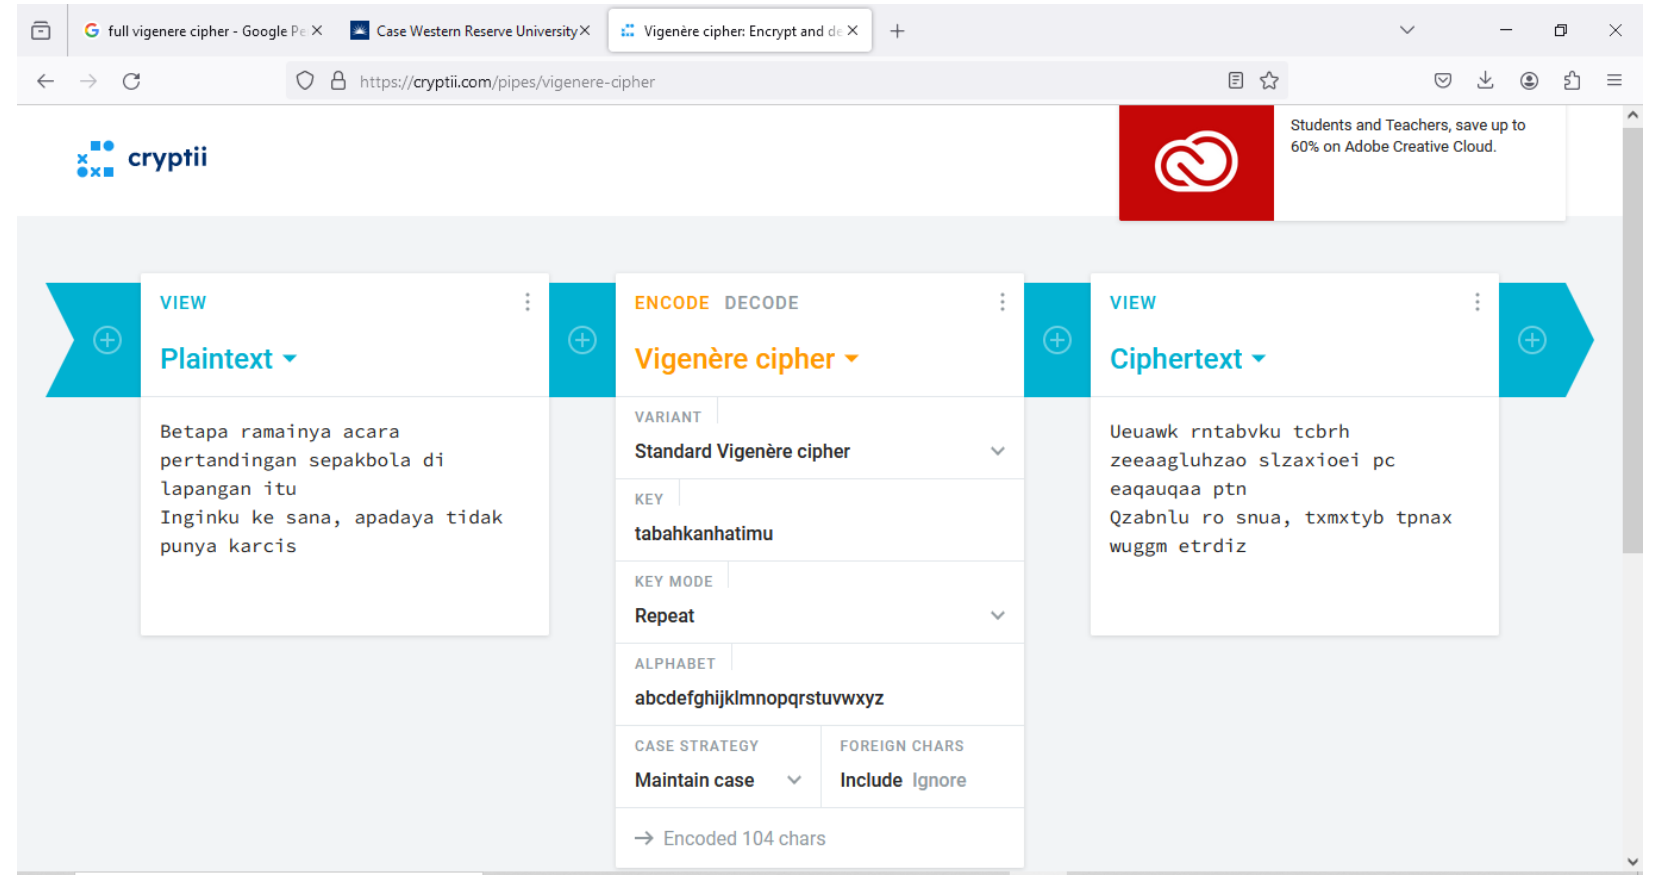
\includegraphics[width=182.70mm,height=240.57mm]{images/llm/page_041_img_01.png}%
\end{textblock*}

\newpage

% --- unit llm 42 ---
% === Halaman 42 (llm) ===

\vspace{240.57mm}

\centering\url{https://www.boxentriq.com/code-breaking/vigenere-cipher}

\vspace{10mm}

% deskripsi: Screenshot halaman web Vigenere Tool dari BoxEntriq yang menampilkan antarmuka untuk melakukan decode, encode, dan auto-solve cipher Vigenere, termasuk input pesan, input kunci, dan opsi Auto Solve.
% bbox normalisasi: [0.0800, 0.1000, 0.9100, 0.9100]
\begin{textblock*}{174.30mm}(16.80mm,29.70mm)
\noindent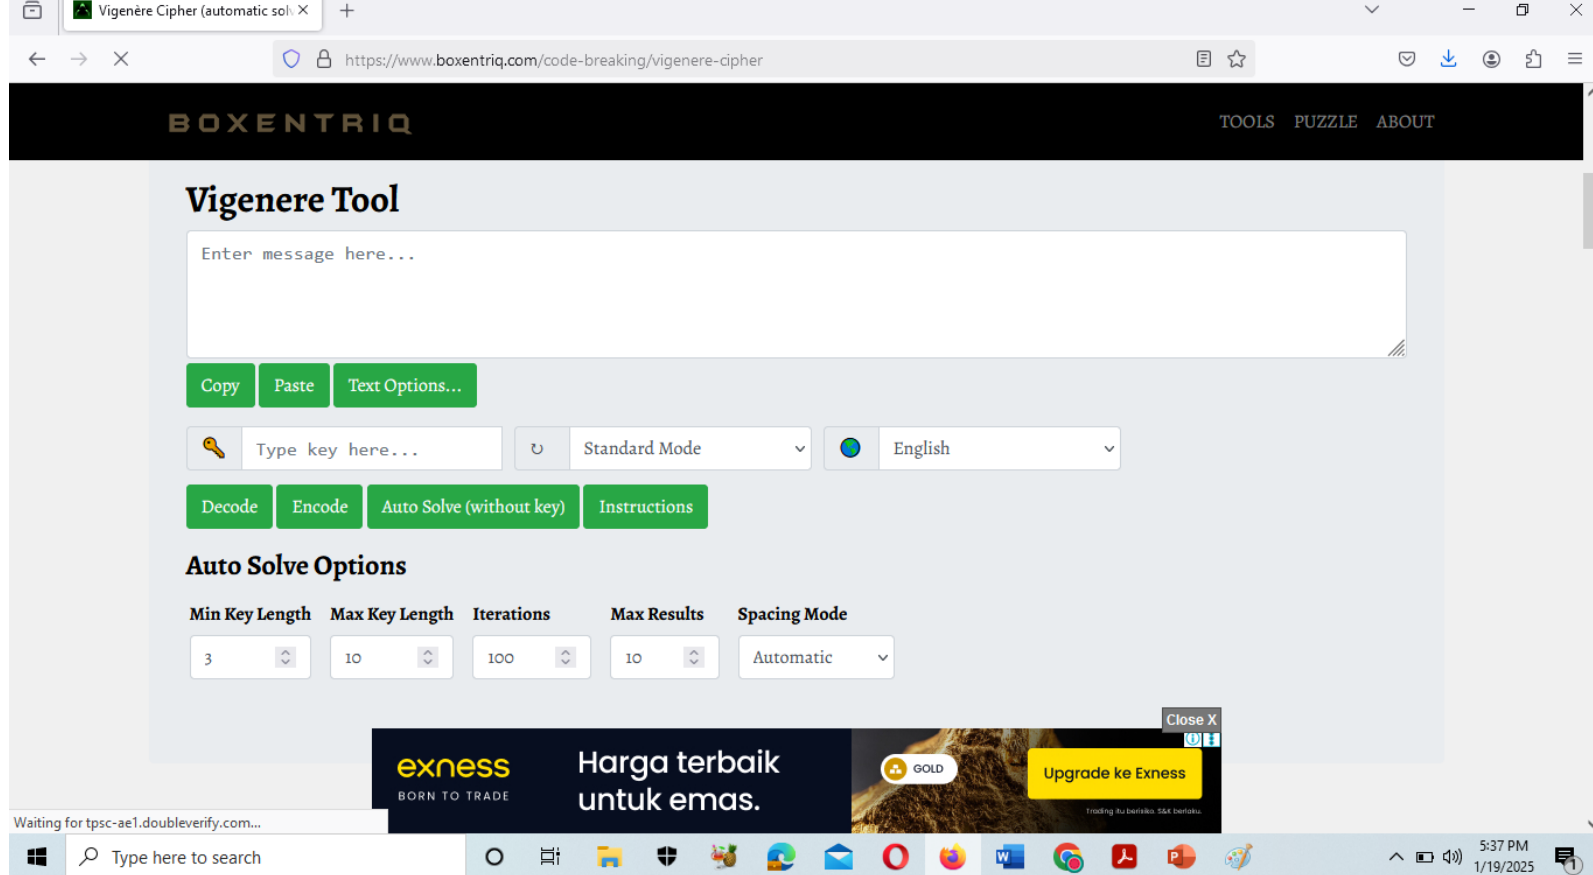
\includegraphics[width=174.30mm,height=240.57mm]{images/llm/page_042_img_01.png}%
\end{textblock*}

\newpage

% --- unit llm 43 ---
% === Halaman 43 (llm) ===

\vspace{234.63mm}

\section*{Vigenere Cipher dalam Python}

% deskripsi: Screenshot kode program Python untuk fungsi enkripsi Vigenere Cipher (Vigenere\_cipher\_encrypt) dan dekripsi (Vigenere\_cipher\_decrypt).
% bbox normalisasi: [0.0000, 0.1200, 0.8000, 0.9100]
\begin{textblock*}{168.00mm}(0.00mm,35.64mm)
\noindent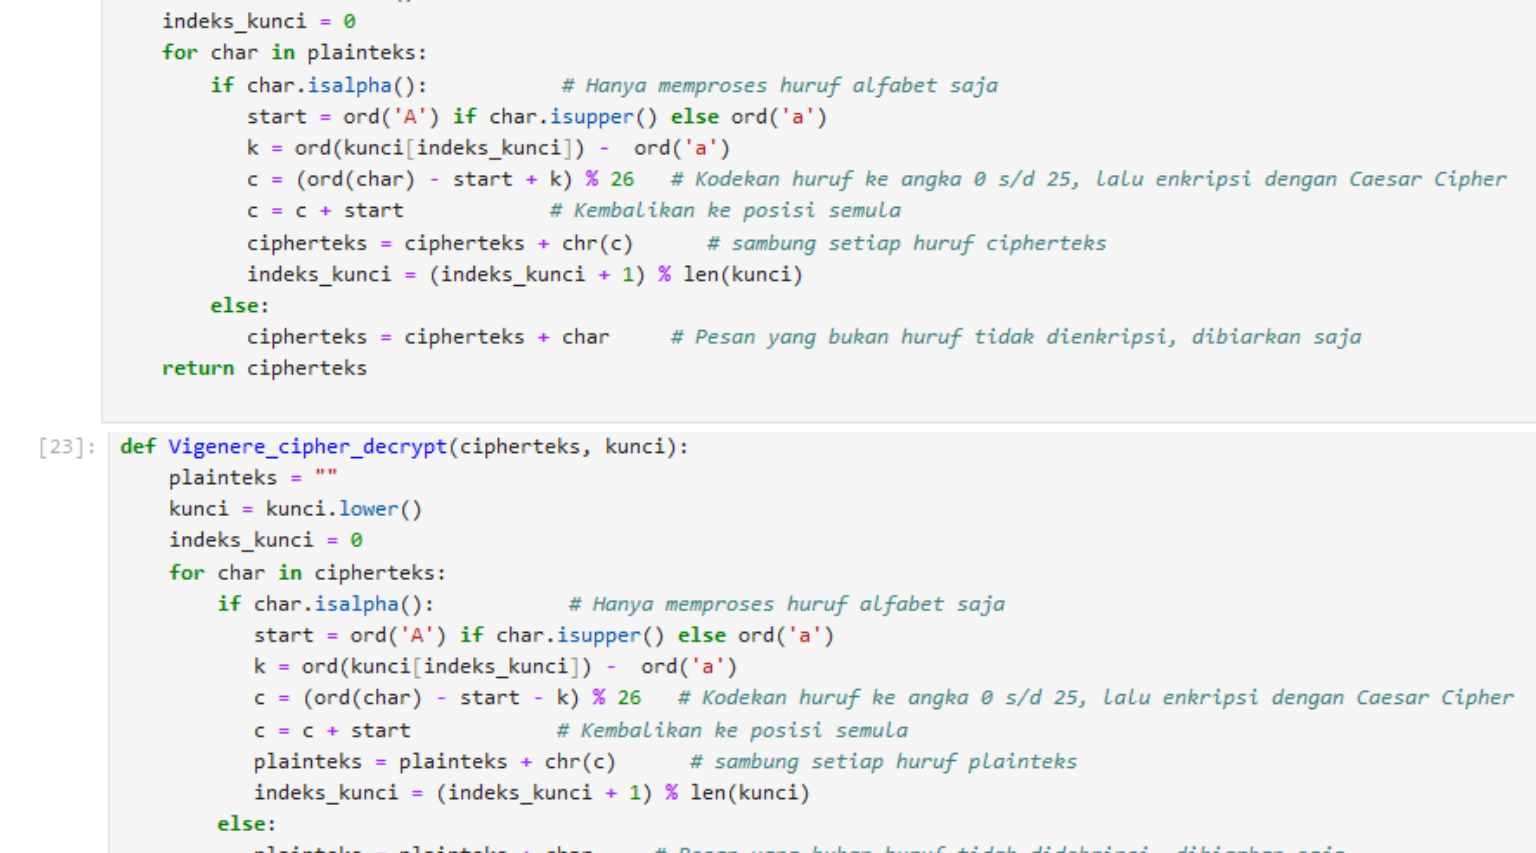
\includegraphics[width=168.00mm,height=234.63mm]{images/llm/page_043_img_01.png}%
\end{textblock*}

\newpage

% --- unit llm 44 ---
% === Halaman 44 (llm) ===

% (tidak ada teks dari model)

% deskripsi: Screenshot kode program Python yang mengimplementasikan enkripsi dan dekripsi menggunakan Vigenere Cipher, lengkap dengan input pengguna dan output hasil eksekusi.
% bbox normalisasi: [0.0600, 0.1700, 0.9300, 0.8400]
\begin{textblock*}{182.70mm}(12.60mm,50.49mm)
\noindent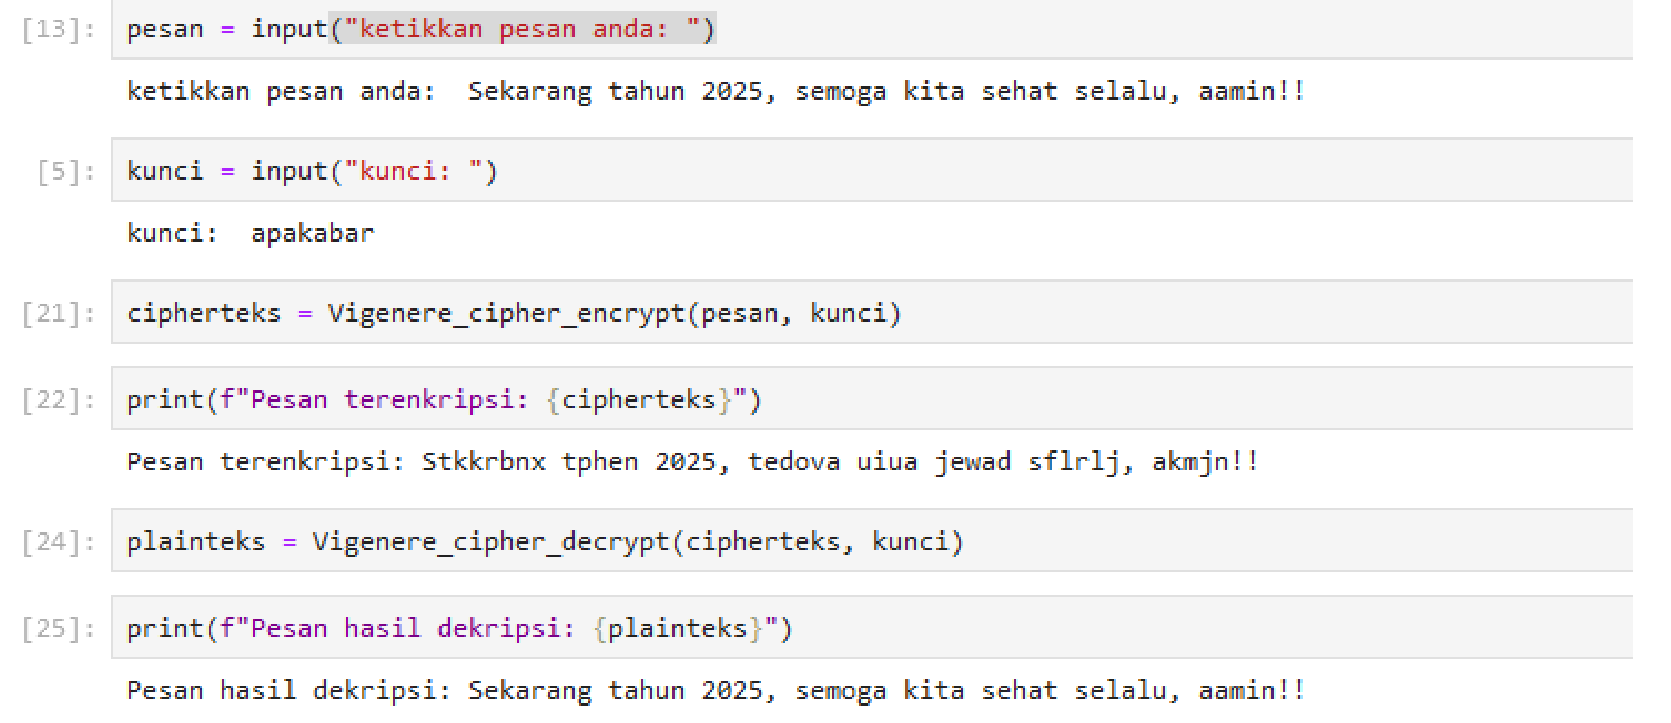
\includegraphics[width=182.70mm,height=198.99mm]{images/llm/page_044_img_01.png}%
\end{textblock*}

\newpage

% --- unit llm 45 ---
% === Halaman 45 (llm) ===

\section*{Extended Vigenere Cipher}

\begin{itemize}
    \item Vigenere cipher untuk 26 huruf dapat dikembangkan untuk enkripsi 256 karakter ASCII
\end{itemize}

\vspace{10mm}

Enkripsi: \[ c_j = E(p_j) = (p_j + k_i) \pmod{256} \]

Dekripsi: \[ p_j = D(c_j) = (c_j - k_i) \pmod{256} \]

\newpage

% --- unit llm 46 ---
% === Halaman 46 (llm) ===

\section*{Latihan}

\begin{itemize}
    \item Ubahlah program Vigenere Cipher di atas sehingga dapat melakukan enkripsi pesan berupa file teks.
\end{itemize}

\newpage

% --- unit llm 47 ---
% === Halaman 47 (llm) ===

\vspace{103.95mm}

\section*{Kriptanalisis Vigenere Cipher}

\begin{itemize}
    \item Friedrich Kasiski adalah orang yang pertama kali memecahkan \textit{Vig\`enere cipher} pada Tahun 1863.
\end{itemize}

\vspace{10mm}

\begin{center}
\begin{tabular}{|l|}
\hline
\textcolor{red}{Friedrich Kasiski} \\
\textcolor{red}{Born: November 29, 1805 @} \textcolor{blue}{Schlochau, Kingdom of Prussia} \\
\textcolor{red}{Died: May 22, 1881 (aged 75) @} \textcolor{blue}{Neustettin, German Empire} \\
\textcolor{red}{Nationality:} \textcolor{blue}{German} \\
\hline
\end{tabular}
\end{center}

\vspace{5mm}

\begin{itemize}
    \item Metodenya dinamakan metode Kasiski
\end{itemize}

% deskripsi: Potret hitam putih Friedrich Kasiski
% bbox normalisasi: [0.8230, 0.0000, 0.9830, 0.3500]
\begin{textblock*}{33.60mm}(172.83mm,0.00mm)
\noindent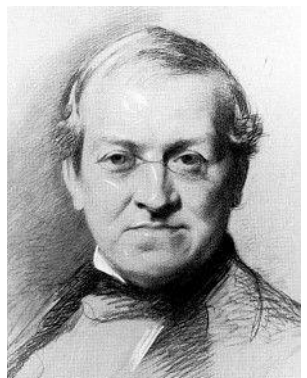
\includegraphics[width=33.60mm,height=103.95mm]{images/llm/page_047_img_01.png}%
\end{textblock*}

\newpage

% --- unit llm 48 ---
% === Halaman 48 (llm) ===

\section*{Metode Kasiski}

\begin{itemize}
    \item Metode Kasiski tidak secara langsung menemukan kunci Vigenere Cipher, tetapi membantu menemukan estimasi \underline{panjang} kunci \textit{Vigenere cipher}.
    \item Metode Kasiski memanfaatkan keuntungan bahwa bahasa Inggris tidak hanya mengandung perulangan huruf,
    \item tetapi juga perulangan pasangan huruf atau tripel huruf, seperti TH, THE, EN, dsb.
    \item Perulangan kelompok huruf ini ada kemungkinan menghasilkan kriptogram yang berulang.
\end{itemize}

\newpage

% --- unit llm 49 ---
% === Halaman 49 (llm) ===

\textbf{Contoh 3:}

\begin{tabular}{lll}
Plainteks & : & \texttt{\color{red}crypto}isshortfor\texttt{\color{red}crypto}graphy} \\
Kunci & : & \texttt{abcdabcdabcdabcdabcdabcdabcdabcd} \\
Cipherteks & : & \texttt{\textbf{CSASTP}KVSIQUTGQU\textbf{CSASTP}IUAQJB} \\
\end{tabular}

\vspace{10mm}

\begin{itemize}
    \item Pada contoh ini, \texttt{crypto} dienkripsi menjadi kriptogram yang sama, yaitu \textbf{CSATP}.
    \item Tetapi kasus seperti ini tidak selalu demikian, misalnya pada contoh berikut ini....
\end{itemize}

\newpage

% --- unit llm 50 ---
% === Halaman 50 (llm) ===

\textbf{Contoh 4:}

\begin{tabular}{ll}
Plainteks & : \texttt{cryptoisshortforcryptography} \\
Kunci & : \texttt{abcdefabcdefabcdefabcdefabcd} \\
Cipherteks & : \texttt{CSASXTITUKWSTGQUCWYQVRKWAQJB} \\
\end{tabular}

\begin{itemize}
    \item Pada contoh di atas, \texttt{crypto} tidak dienkripsi menjadi kriptogram yang sama. 
    \item Mengapa bisa demikian?
\end{itemize}

\newpage

% --- unit llm 51 ---
% === Halaman 51 (llm) ===

\begin{itemize}
    \item Secara intuitif: jika jarak antara dua buah \textit{string} yang berulang di dalam plainteks merupakan kelipatan dari panjang kunci,
    \item maka \textit{string} yang sama tersebut akan muncul menjadi kriptogram yang sama pula di dalam cipherteks.
    \item Pada Contoh 1,
    \begin{itemize}
        \item kunci = \texttt{abcd}
        \item panjang kunci = 4
        \item jarak antara dua \texttt{crypto} yang berulang = 16
        \item $16 = \text{kelipatan } 4$
    \end{itemize}
\end{itemize}

\vspace{10mm}

$\therefore$ \texttt{crypto} dienkripsi menjadi kriptogram yang sama

% deskripsi: Ilustrasi proses enkripsi Vigenere cipher yang menunjukkan plainteks 'cryptoisshortforcryptography' dengan kata 'crypto' yang berulang pada jarak 16 karakter, kunci 'abcd' yang berulang, dan hasil cipherteks yang menunjukkan pola pengulangan 'CSASTP'.
% bbox normalisasi: [0.4200, 0.3900, 0.8900, 0.6200]
\begin{textblock*}{98.70mm}(88.20mm,115.83mm)
\noindent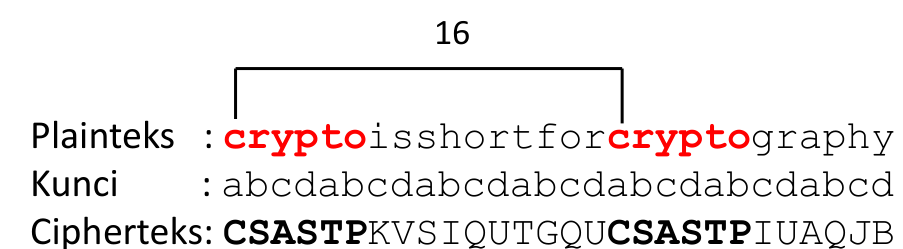
\includegraphics[width=98.70mm,height=68.31mm]{images/llm/page_051_img_01.png}%
\end{textblock*}

\newpage

% --- unit llm 52 ---
% === Halaman 52 (llm) ===

\vspace{11.88mm}

\begin{itemize}
    \item Pada Contoh 2, 
    \begin{itemize}
        \item kunci = \texttt{abcdef}
        \item panjang kunci = 6
        \item jarak antara dua \texttt{crypto} yang berulang = 16
        \item 16 bukan kelipatan 6
    \end{itemize}
    $\therefore$ \texttt{crypto} tidak dienkripsi menjadi kriptogram yang sama
    
    \vspace{10mm}
    
    \item Goal metode Kasiski: mencari dua atau lebih kriptogram yang berulang untuk menentukan panjang kunci.
\end{itemize}

% deskripsi: Ilustrasi proses enkripsi Vigenere dengan teks plaintext, kunci, dan cipherteks, menunjukkan jarak antara kata 'crypto' yang berulang adalah 16 karakter.
% bbox normalisasi: [0.0600, 0.1080, 0.9400, 0.9120]
\begin{textblock*}{184.80mm}(12.60mm,32.08mm)
\noindent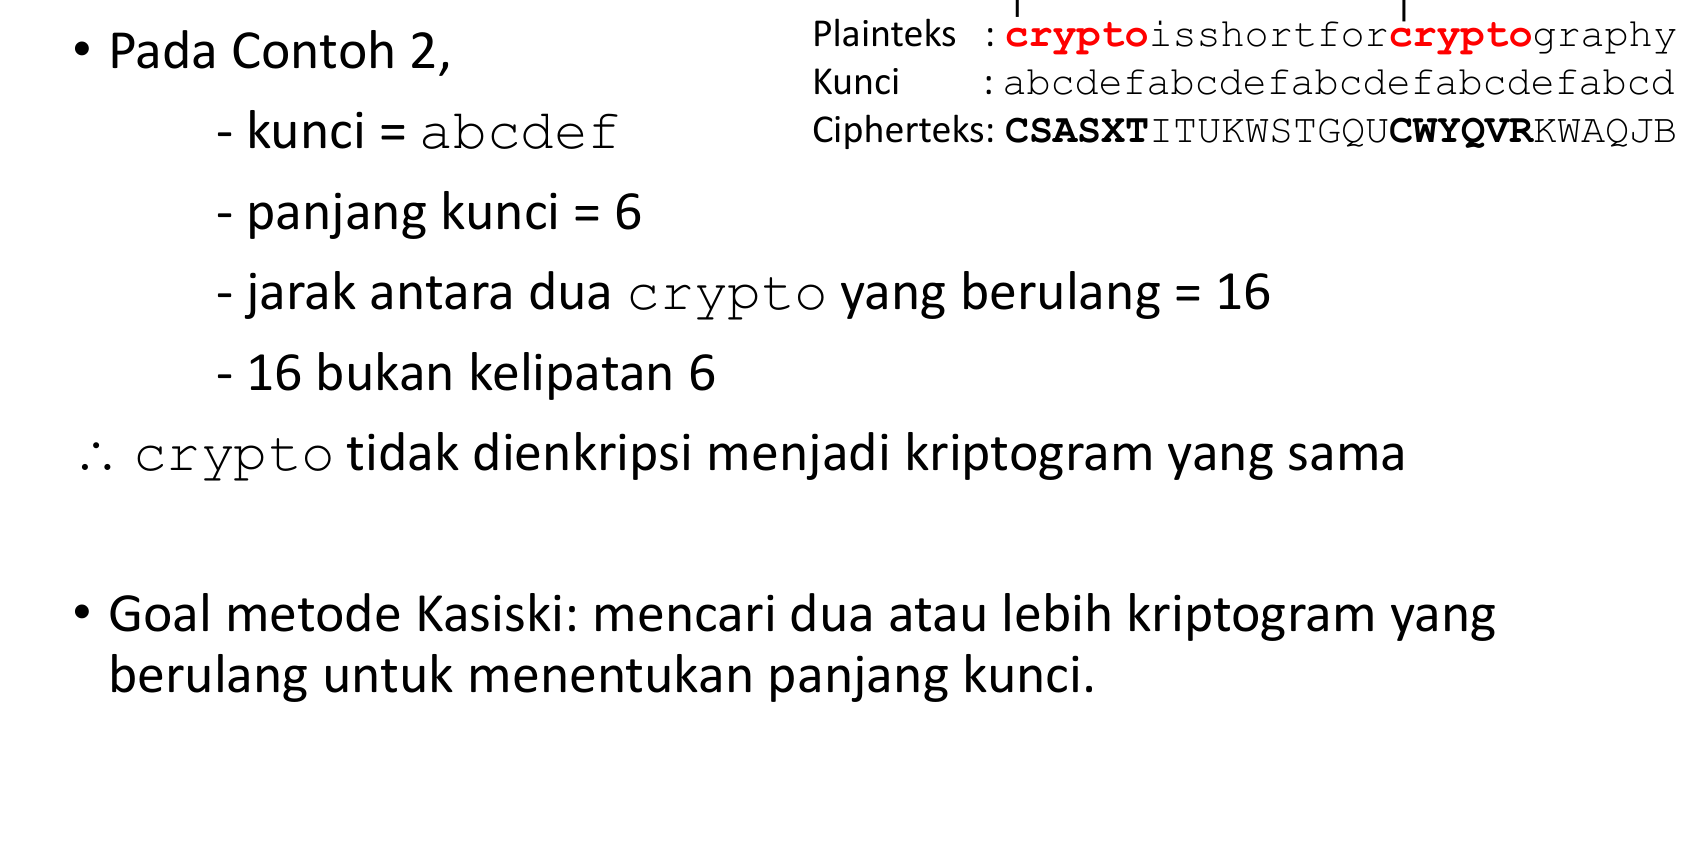
\includegraphics[width=184.80mm,height=238.79mm]{images/llm/page_052_img_01.png}%
\end{textblock*}

% deskripsi: Contoh perhitungan jarak antara dua kata 'crypto' yang berulang dalam plaintext yang diberi label angka 16.
% bbox normalisasi: [0.4800, 0.2000, 0.9400, 0.2400]
\begin{textblock*}{96.60mm}(100.80mm,59.40mm)
\noindent
\includegraphics[width=96.60mm,height=11.88mm]{images/llm/page_052_img_02.png}%
\end{textblock*}

% bbox perkiraan otomatis: Ilustrasi proses enkripsi Vigenere dengan teks plaintext, kunci, dan cipherteks, menunjukkan jarak antara kata 'crypto' yang berulang adalah 16 karakter.

\newpage

% --- unit llm 53 ---
% === Halaman 53 (llm) ===

Langkah-langkah metode Kasiski:

\begin{enumerate}
  \item Temukan semua kriptogram yang berulang di dalam cipherteks (pesan yang panjang biasanya mengandung kriptogram yang berulang).
  \item Hitung jarak antara kriptogram yang berulang
  \item Hitung semua faktor (pembagi) dari jarak tersebut (faktor pembagi menyatakan panjang kunci yang mungkin ).
  \item Tentukan irisan dari himpunan faktor pembagi tersebut. Nilai yang muncul di dalam irisan menyatakan angka yang muncul pada semua faktor pembagi dari jarak-jarak tersebut . Nilai tersebut mungkin adalah panjang kunci.
\end{enumerate}

\newpage

% --- unit llm 54 ---
% === Halaman 54 (llm) ===

\begin{itemize}
  \item Contoh:
  \vspace{5mm}
  \textcolor{red}{DYDUXRMH}TVDV\textcolor{cyan}{NQD}QNW\textcolor{red}{DYDUXRMH}ARTJGW\textcolor{cyan}{NQD}
\end{itemize}

Kriptogram yang berulang: \textbf{DYUDUXRMH} dan \textbf{NQD}.

Jarak antara dua buah perulangan \textbf{DYUDUXRMH} $= 18$.
Semua faktor pembagi $18 : \{18, 9, 6, 3, 2\}$

Jarak antara dua buah perulangan \textbf{NQD} $= 20$.
Semua faktor pembagi $20 : \{20, 10, 5, 4, 2\}$.

Irisan dari kedua buah himpunan tersebut adalah 2
Panjang kunci kemungkinan besar adalah 2.

\newpage

% --- unit llm 55 ---
% === Halaman 55 (llm) ===

\begin{itemize}
    \item Setelah panjang kunci diketahui, maka langkah berikutnya menentukan huruf-huruf kunci
    \item Huruf-huruf kunci dapat ditentukan dengan menggunakan \textit{exhaustive key search}
    \item Jika panjang kunci $= p$, maka jumlah kunci yang harus dicoba sampai menemukan kunci yang benar adalah adalah maksimal $26^p$ kali.
    \item Namun lebih sangkil menemukan huruf-huruf kunci dengan menggunakan teknik analisis frekuensi.
\end{itemize}

\newpage

% --- unit llm 56 ---
% === Halaman 56 (llm) ===

Langkah-langkahnya sbb:

\begin{enumerate}
  \item Misalkan panjang kunci yang sudah berhasil dideduksi adalah $n$. Setiap huruf berjarak $n$ pasti dienkripsi dengan huruf kunci yang sama. Kelompokkan setiap huruf berjarak $n$ bersama-sama sehingga kriptanalis memiliki $n$ buah \"pesan\", masing-masing \"pesan\" dienkripsi dengan huruf kunci yang sama dengan \textit{cipher} abjad-tunggal (dalam hal ini \textit{Caesar cipher}).
  \item Tiap-tiap pesan dari hasil langkah 1 dapat dipecahkan dengan metode analisis frekuensi.
  \item Dari hasil langkah 2 kriptanalis dapat menyusun huruf-huruf kunci. Atau, kriptanalis dapat menerka kata yang membantu untuk memecahkan cipherteks
\end{enumerate}

\newpage

% --- unit llm 57 ---
% === Halaman 57 (llm) ===

\begin{itemize}
    \item Contoh:
\end{itemize}

\vspace{5mm}

Kriptogram yang berulang adalah \textbf{LJV}

\begin{align*}
    \text{Jarak \textbf{LJV} ke-1 dengan \textbf{LJV} ke-2} &= 15 \\
    \text{Jarak \textbf{LJV} ke-2 dengan \textbf{LJV} ke-3} &= 15 \\
    \text{Jarak \textbf{LJV} ke-3 dengan \textbf{LJV} ke-4} &= 15 \\
    \text{Jarak \textbf{LJV} ke-4 dengan \textbf{LJV} ke-5} &= 10 \\
    \text{Jarak \textbf{LJV} ke-5 dengan \textbf{LJV} ke-6} &= 10
\end{align*}

Faktor pembagi $15 = \{3, 5, 15\}$

Faktor pembagi $10 = \{2, 5, 10\}$

Irisan kedua himpunan ini $= 5$. Jadi, panjang kunci diperkirakan $= 5$

% deskripsi: Teks kriptogram dengan penanda angka 1 sampai 6 di atas pola yang berulang 'LJV'.
% bbox normalisasi: [0.1010, 0.1430, 0.9180, 0.3440]
\begin{textblock*}{171.57mm}(21.21mm,42.47mm)
\noindent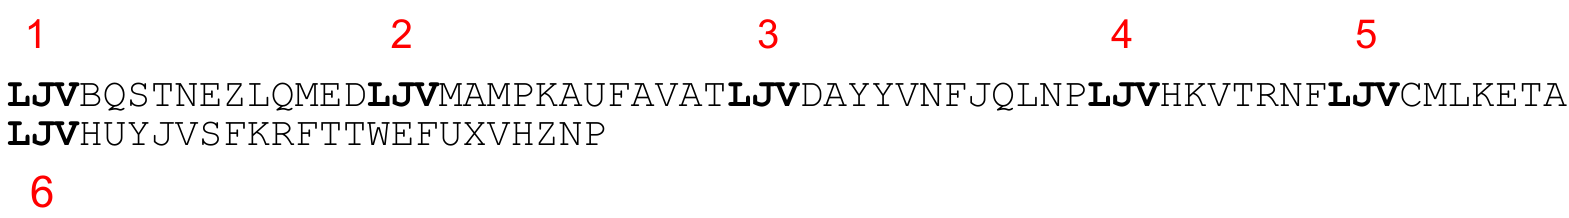
\includegraphics[width=171.57mm,height=59.70mm]{images/llm/page_057_img_01.png}%
\end{textblock*}

\newpage

% --- unit llm 58 ---
% === Halaman 58 (llm) ===

\begin{itemize}
    \item Kelompokkan "pesan" setiap berjarak 5, dimulai dari huruf cipherteks pertama, kedua, dan seterusnya. Setiap huruf pada posisi berjarak 5 pasti dienkripsi dengan huruf kunci yang sama.
\end{itemize}

\vspace{10mm}

\begin{tabular}{l l} 
Kelompok & Pesan \\
\hline
1 & LSLLMFLYJLVLLLYKWV \\
2 & JTQJPAJYQJTJKJJREH \\
3 & VNMVKVVVVLVRVEVFFZ \\
4 & BEEMAADNNHNCTHSTUN \\
5 & QZDAUTAFPKFMAUFTXP \\
\end{tabular}

\vspace{5mm}

\begin{tabular}{l} 
Huruf paling sering muncul \\
\hline
L \\
J \\
V \\
N \\
A \\
\end{tabular}

% deskripsi: Contoh pengelompokan cipherteks dengan huruf berwarna untuk menunjukkan pola pengulangan setiap 5 karakter.
% bbox normalisasi: [0.0500, 0.2900, 0.9200, 0.4500]
\begin{textblock*}{182.70mm}(10.50mm,86.13mm)
\noindent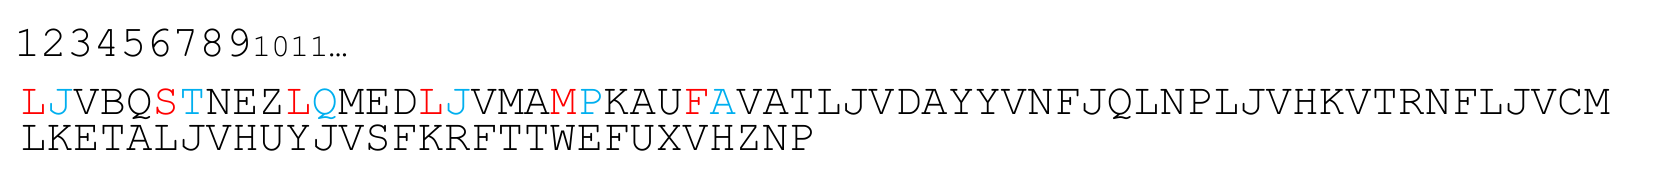
\includegraphics[width=182.70mm,height=47.52mm]{images/llm/page_058_img_01.png}%
\end{textblock*}

\newpage

% --- unit llm 59 ---
% === Halaman 59 (llm) ===

\begin{itemize}
    \item Dalam Bahasa Inggris, 10 huruf yang yang paling sering muncul adalah E, T, A, O, I, N, S, H, R, dan D,
    \item Triplet yang paling sering muncul adalah THE. Karena \textbf{LJV} paling sering muncul di dalam cipherteks, maka dari 10 huruf tsb semua kemungkinan kata 3-huruf dibentuk dan kata yang yang cocok untuk \textbf{LJV} adalah \underline{THE}.
    \item Jadi, kita dapat menerka bahwa \textbf{LJV} mungkin adalah \underline{THE}.
    \item Huruf-huruf kunci lainnya dicoba dengan menerka dan menguji coba.
    \item Dari sini kita buat tabel yang memetakan huruf plainteks dengan cipherteks dan huruf-huruf kuncinya (ingatlah bahwa setiap nilai numerik dari huruf kunci menyatakan jumlah pergeseran huruf pada \textit{Caesar cipher}):
\end{itemize}

\newpage

% --- unit llm 60 ---
% === Halaman 60 (llm) ===

\vspace{196.02mm}

Jadi, kuncinya adalah \texttt{SCRAM}

% deskripsi: Tabel yang menunjukkan pemetaan antara huruf plainteks, huruf cipherteks, dan huruf kunci beserta nilai numeriknya untuk lima kelompok data.
% bbox normalisasi: [0.0700, 0.1200, 0.8800, 0.7800]
\begin{textblock*}{170.10mm}(14.70mm,35.64mm)
\noindent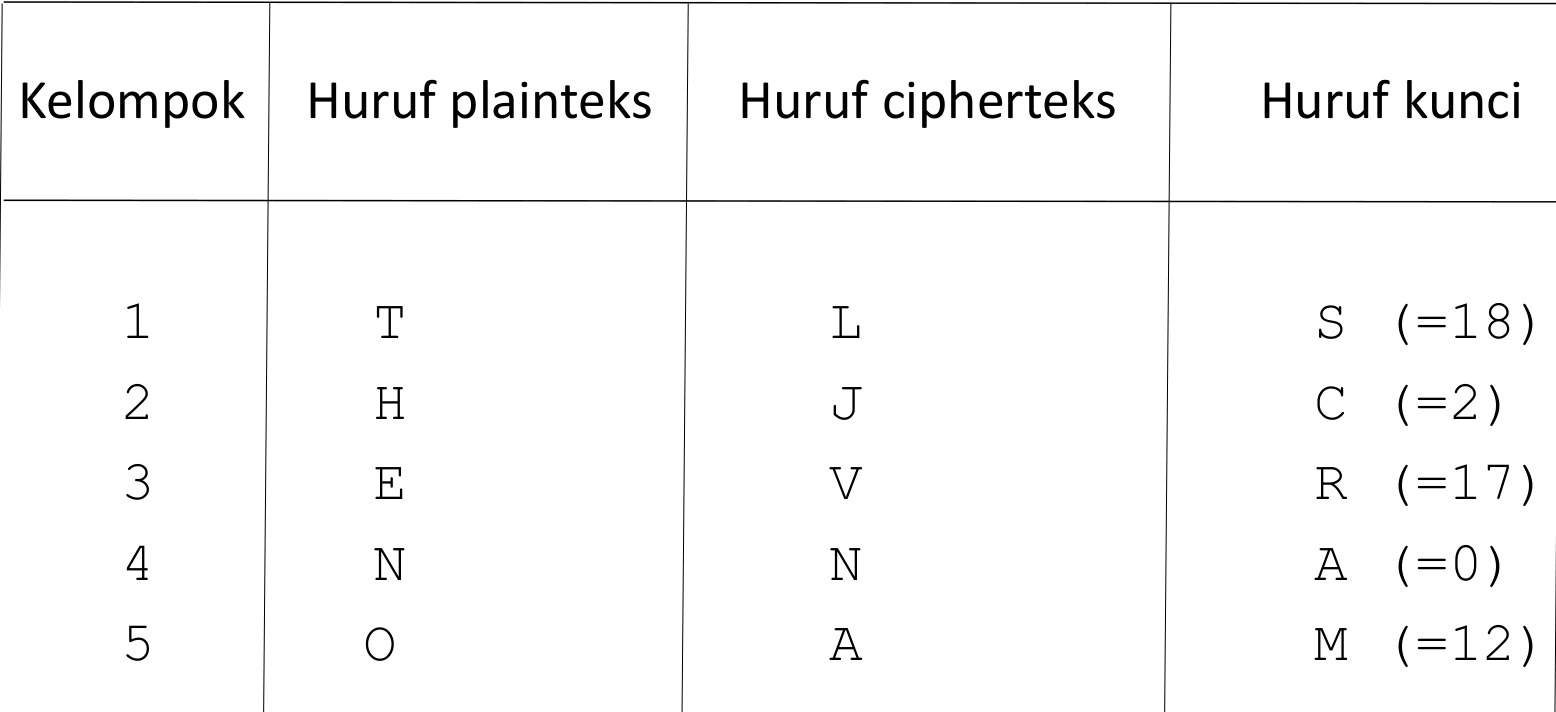
\includegraphics[width=170.10mm,height=196.02mm]{images/llm/page_060_img_01.png}%
\end{textblock*}

\newpage

% --- unit llm 61 ---
% === Halaman 61 (llm) ===

\begin{itemize}
    \item Dengan menggunakan kunci SCRAM cipherteks berhasil didekripsi menjadi:
    
    \begin{center}
    \begin{tabular}{l}
    THEBE ARWEN TOVER THEMO UNTAI NYEAH \\
    THEDO GWENT ROUND THEHY DRANT THECA \\
    TINTO THEHI GHEST SPOTH ECOUL DFIND
    \end{tabular}
    \end{center}
    
    \item Lakukan post-processing untuk menghasilkan kalimat yang lebih jelas:
    
    \begin{center}
    \begin{tabular}{l}
    THE BEAR WENT OVER THE MOUNTAIN YEAH \\
    THE DOG WENT ROUND THE HYDRANT \\
    THE CAT INTO THE HIGHEST SPOT HE COULD FIND
    \end{tabular}
    \end{center}
\end{itemize}

\newpage

% --- unit llm 62 ---
% === Halaman 62 (llm) ===

\section*{Varian Vigenere Cipher}

Untuk mengatasi serangan dengan metode Kasiski, maka dibuat varian Vigenere Cipher sebagai berikut:

\begin{enumerate}
    \item \textcolor{red}{Full Vig\grave{e}n\grave{e}re cipher}
    \begin{itemize}
        \item Setiap baris di dalam tabel tidak menyatakan pergeseran huruf, tetapi merupakan permutasi huruf-huruf alfabet (lihat contoh table pada halaman berikut).
        \item Tabel tersebut harus dirahasiakan.
        \item Proses enkripsi dan dekripsi tetap sama seperti Vigenere standard:
    \end{itemize}
\end{enumerate}

\newpage

% --- unit llm 63 ---
% === Halaman 63 (llm) ===

\vspace{219.78mm}

Contoh sebuah full Vigen\`ere square

% deskripsi: Tabel Vigen\`ere square yang berisi alfabet A-Z pada baris dan kolom, dengan setiap sel berisi karakter hasil enkripsi pergeseran alfabet.
% bbox normalisasi: [0.2900, 0.2300, 0.7400, 0.9700]
\begin{textblock*}{94.50mm}(60.90mm,68.31mm)
\noindent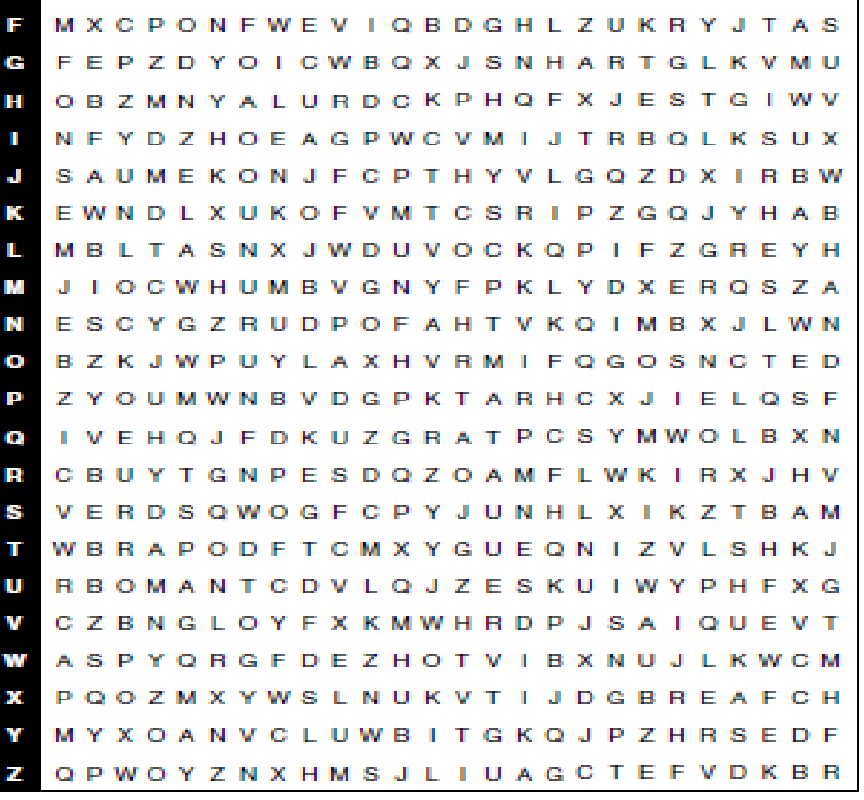
\includegraphics[width=94.50mm,height=219.78mm]{images/llm/page_063_img_01.png}%
\end{textblock*}

\newpage

% --- unit llm 64 ---
% === Halaman 64 (llm) ===

\textcolor{red}{\textbf{2. Auto-Key Vig\`en\`ere cipher}}

\begin{itemize}
    \item Jika panjang kunci lebih kecil dari panjang plainteks, maka kunci disambung dengan plainteks tersebut.
    \item Misalnya,
    \begin{itemize}
        \item Pesan: \texttt{negara penghasil minyak mentah di dunia}
        \item Kunci: \texttt{INDO}
    \end{itemize}
    maka kunci tersebut disambung dengan plainteks semula sehingga panjang kunci menjadi sama dengan panjang plainteks:
    \begin{itemize}
        \item Plainteks: \texttt{negarapenghasilminyakmentahdidunia}
        \item Kunci: \texttt{INDONEGARAPENGHASILMINYAKMENTAHDID}
        \item Cipherteks: \texttt{VRJOEEVEEGWEFOSMAVJMSZCNDMLQBDBQQD}
    \end{itemize}
\end{itemize}

\newpage

% --- unit llm 65 ---
% === Halaman 65 (llm) ===

\textcolor{red}{\textbf{3. Running-Key Vig\`enere cipher}}

\begin{itemize}
    \item Kunci adalah string yang sangat panjang yang diambil dari teks bermakna (misalnya naskah proklamasi, naskah Pembukaan UUD 1945, terjemahan ayat di dalam kitab suci, dan lain-lain).
    \item Misalnya,
    \begin{itemize}
        \item Pesan: \texttt{negarapenghasilminyakmentahdidunia}
        \item Kunci: \texttt{KERAKYATANYANGDIPIMPINOLEHHIKMATPE}
    \end{itemize}
    \item Selanjutnya enkripsi dan dekripsi dilakukan seperti Vigenere cipher biasa.
\end{itemize}

\newpage

% --- unit llm 66 ---
% === Halaman 66 (llm) ===

\section*{C. Playfair Cipher}

\begin{itemize}
    \item Ditemukan oleh Sir Charles Wheatstone namun dipromosikan oleh Baron Lyon Playfair pada tahun 1854.
\end{itemize}

\vspace{20mm}

\begin{center}
    Sir Charles Wheatstone \hfill Baron Lyon Playfair
\end{center}

% deskripsi: Foto potret Sir Charles Wheatstone
% bbox normalisasi: [0.2640, 0.4600, 0.4040, 0.7660]
\begin{textblock*}{29.40mm}(55.44mm,136.62mm)
\noindent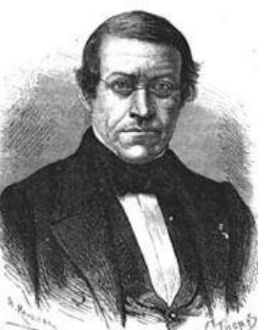
\includegraphics[width=29.40mm,height=90.88mm]{images/llm/page_066_img_01.png}%
\end{textblock*}

% deskripsi: Foto potret Baron Lyon Playfair
% bbox normalisasi: [0.6010, 0.4530, 0.7410, 0.7600]
\begin{textblock*}{29.40mm}(126.21mm,134.54mm)
\noindent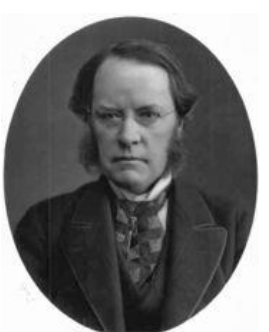
\includegraphics[width=29.40mm,height=91.18mm]{images/llm/page_066_img_02.png}%
\end{textblock*}

\newpage

% --- unit llm 67 ---
% === Halaman 67 (llm) ===

\section*{Lyon Playfair, 1st Baron Playfair}

\vspace{204.34mm}

From Wikipedia, the free encyclopedia\newline
(Redirected from Lord Playfair)

\textbf{Lyon Playfair, 1st Baron Playfair} (1 May 1818 -- 29 May 1898) was a British scientist and Liberal politician who was Postmaster-General from 1873 to 1874.

\vspace{10mm}

\subsection*{Early life}

Playfair was born at Chunar, Bengal, the son of George Playfair (1781--1845), the chief inspector-general of hospitals in that region, and Janet Ross (1795--1862), daughter of John Ross. The family was fairly middle class with strong academic roots in University of St Andrews, his grandfather being Rev Prof James Playfair, Principal of the University of St Andrews. All of Playfair's siblings were sent back to Scotland to avoid the hazards of an Indian upbringing. Playfair was named after his uncle, Sir Hugh Lyon Playfair, and was educated at the University of St Andrews, the Andersonian Institute in Glasgow, and the University of Edinburgh. After going to Calcutta at the end of 1837, he became private laboratory assistant to Thomas Graham at University College London and in 1839 went to work under Justus Liebig at the University of Giessen.

% deskripsi: Infobox Wikipedia mengenai Lord Playfair yang berisi foto potret dan detail jabatan sebagai Postmaster General.
% bbox normalisasi: [0.5330, 0.2440, 0.7550, 0.9320]
\begin{textblock*}{46.62mm}(111.93mm,72.47mm)
\noindent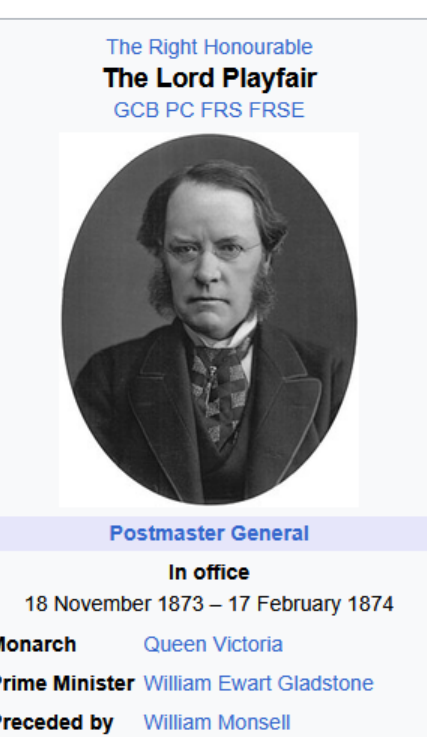
\includegraphics[width=46.62mm,height=204.34mm]{images/llm/page_067_img_01.png}%
\end{textblock*}

\newpage

% --- unit llm 68 ---
% === Halaman 68 (llm) ===

\begin{itemize}
    \item \textit{Playfair cipher} termasuk ke dalam kelompok \textit{polygram cipher}
    \item Pada \textit{polygram cipher}, satu blok huruf plainteks disubstitusi dengan satu blok huruf cipherteks.
    \item Jika satu blok panjangnya 2 huruf, maka ia disebut digram (\textit{bigram}), jika 3 huruf disebut trigram, dst. \textit{Playfair cipher} melakukan enkripsi/dekripsi dalam bentuk bigram.

    Misalnya, bigram \texttt{AS} diganti dengan \texttt{RT}, \texttt{BY} diganti dengan \texttt{SL}
\end{itemize}

\newpage

% --- unit llm 69 ---
% === Halaman 69 (llm) ===

\begin{itemize}
    \item Kunci enkripsi/dekripsi pada Playfair cipher disusun berbentuk matriks berukuran $5 \times 5$
    \item Setiap elemen matriks adalah huruf-huruf alfabet A..Z
    \item Karena ada 25 elemen matriks, dan ada 26 huruf alfabet, maka ada satu huruf alfabet dibuang, yaitu huruf J
\end{itemize}

\vspace{10mm}

\begin{itemize}
    \item Jumlah kemungkinan matriks kunci yang bisa dibentuk:
    \[ 25! = 15.511.043.330.985.984.000.000 \]
\end{itemize}

% deskripsi: Matriks kunci Playfair cipher ukuran 5x5 yang berisi huruf-huruf alfabet acak.
% bbox normalisasi: [0.3110, 0.4640, 0.5280, 0.7750]
\begin{textblock*}{45.57mm}(65.31mm,137.81mm)
\noindent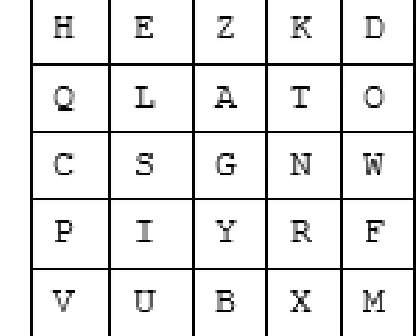
\includegraphics[width=45.57mm,height=92.37mm]{images/llm/page_069_img_01.png}%
\end{textblock*}

\newpage

% --- unit llm 70 ---
% === Halaman 70 (llm) ===

\textbf{Alasan mengapa huruf J dibuang:}

\begin{enumerate}
    \item Matriks Playfair hanya $5\times 5$
    Playfair cipher menggunakan tabel $5\times 5$, jadi hanya bisa memuat 25 huruf. Sementara alfabet latin ada 26 huruf (A--Z). Artinya satu huruf harus "dikorbankan".

    \item I dan J dianggap mirip secara historis
    Secara historis, dalam alfabet Latin lama, I dan J tidak dibedakan. J dianggap hanya variasi dari I. Karena itu, Playfair menggabungkan I dan J. Huruf J dihilangkan. Semua J dalam plaintext diganti menjadi I
    Contoh: JALAN $\rightarrow$ IALAN

    \item Dampaknya ke proses enkripsi/dekripsi
    Saat enkripsi: setiap I diperlakukan sebagai I. Saat dekripsi: huruf I bisa berarti I atau J, tergantung konteks bahasa. Ini tidak mengurangi keamanan, karena Playfair sudah bersifat substitusi digraf
    Ambiguitas kecil ini masih bisa diselesaikan lewat konteks

    \item Apakah bisa buang huruf lain?
    Bisa saja secara teori, tapi I/J paling masuk akal secara linguistik
    Sudah jadi standar konvensi Playfair. Memudahkan implementasi dan pembacaan hasil
\end{enumerate}

\begin{flushright}
Sumber: ChatGPT
\end{flushright}

\newpage

% --- unit llm 71 ---
% === Halaman 71 (llm) ===

Kunci dapat dipilih dari sebuah kalimat yang mudah diingat, misalnya:

\begin{center}
JALAN GANESHA SEPULUH
\end{center}

Buang huruf yang berulang dan huruf $J$ jika ada:

\begin{center}
ALNGESHPU
\end{center}

Lalu tambahkan huruf-huruf yang belum ada (kecuali $J$):

\vspace{69.50mm}

\begin{center}
ALNGESHPUBCDFIKMOQRTVWXYZ
\end{center}

Masukkan ke dalam bujursangkar:

\vspace{10mm}

% deskripsi: Tabel bujursangkar yang berisi huruf-huruf hasil proses penyusunan kunci kriptografi.
% bbox normalisasi: [0.3170, 0.6530, 0.5120, 0.8870]
\begin{textblock*}{40.95mm}(66.57mm,193.94mm)
\noindent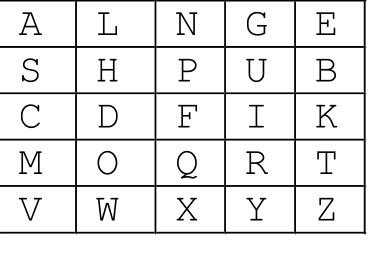
\includegraphics[width=40.95mm,height=69.50mm]{images/llm/page_071_img_01.png}%
\end{textblock*}

\newpage

% --- unit llm 72 ---
% === Halaman 72 (llm) ===

Pesan yang akan dienkripsi diatur terlebih dahulu sebagai berikut (langkah \textit{preprocessing}):

\begin{enumerate}
  \item Buang semua spasi di dalam pesan
  \item Ganti huruf j (bila ada) dengan i. Contoh: jalan $\rightarrow$ ialan
  \item Tulis pesan dalam pasangan huruf (\textit{bigram}).
  \item Jangan sampai ada bigram dengan pasangan huruf yang sama. Jika ada, sisipkan x di tengahnya
  \item Jika jumlah huruf di dalam pesan ganjil, tambahkan huruf x pada bigram terakhir
\end{enumerate}

\newpage

% --- unit llm 73 ---
% === Halaman 73 (llm) ===

Contoh plainteks: \texttt{temui ibu nanti malam}

$\rightarrow$ Tidak ada huruf j, maka langsung tulis pesan dalam pasangan huruf (setelah semua spasi dibuang):

\texttt{te mu ii bu na nt im al am}

$\rightarrow$ Ada bigram dengan huruf yang berulang (\texttt{ii}), sisipkan huruf x di tengahnya:

\texttt{te mu ix ib un an ti ma la m}

$\rightarrow$ Tambahkan huruf x jika bigram terakhir hanya satu huruf:

\texttt{te mu ix ib un an ti ma la mx}

\newpage

% --- unit llm 74 ---
% === Halaman 74 (llm) ===

Algoritma enkripsi:\
1. Jika dua huruf terdapat pada baris kunci yang sama maka tiap huruf diganti dengan huruf di kanannya (bersifat siklik).

\vspace{10mm}

\vspace{10mm}

Cipherteks: FK \hfill Cipherteks: RM

% deskripsi: Ilustrasi proses enkripsi bigram 'di' menggunakan tabel Playfair, di mana huruf 'd' dan 'i' berada di baris yang sama sehingga diganti oleh huruf di kanannya yaitu 'f' dan 'k'.
% bbox normalisasi: [0.0900, 0.3700, 0.3200, 0.8000]
\begin{textblock*}{48.30mm}(18.90mm,109.89mm)
\noindent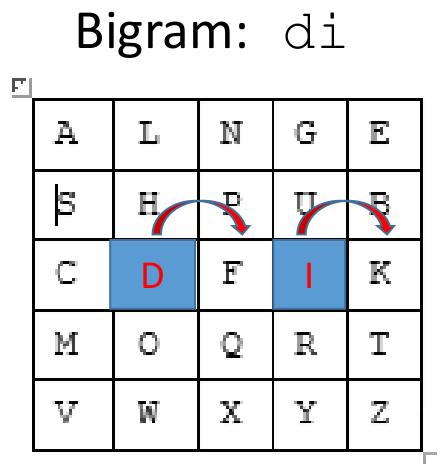
\includegraphics[width=48.30mm,height=127.71mm]{images/llm/page_074_img_01.png}%
\end{textblock*}

% deskripsi: Ilustrasi proses enkripsi bigram 'qt' menggunakan tabel Playfair, di mana huruf 'q' dan 't' berada di baris yang sama sehingga diganti oleh huruf di kanannya yaitu 'r' dan 'm' (siklik kembali ke awal baris).
% bbox normalisasi: [0.5700, 0.3700, 0.8200, 0.8000]
\begin{textblock*}{52.50mm}(119.70mm,109.89mm)
\noindent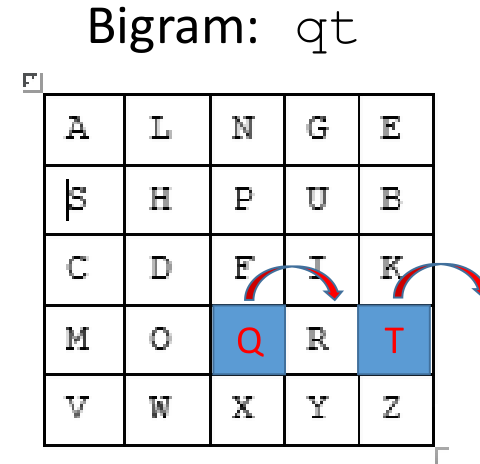
\includegraphics[width=52.50mm,height=127.71mm]{images/llm/page_074_img_02.png}%
\end{textblock*}

\newpage

% --- unit llm 75 ---
% === Halaman 75 (llm) ===

2. Jika dua huruf terdapat pada kolom kunci yang sama maka tiap huruf diganti dengan huruf di bawahnya (bersifat siklik).

\vspace{10mm}

\vspace{10mm}

Cipherteks: PX \hspace{5cm} Cipherteks: WL

% deskripsi: Ilustrasi kriptografi Playfair untuk kasus bigram 'nq' di mana kedua huruf berada dalam satu kolom, menunjukkan pergeseran huruf ke bawah secara siklik untuk menghasilkan cipherteks PX.
% bbox normalisasi: [0.1200, 0.3000, 0.3400, 0.7500]
\begin{textblock*}{46.20mm}(25.20mm,89.10mm)
\noindent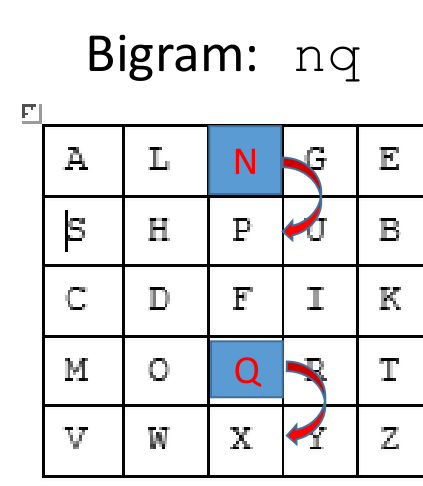
\includegraphics[width=46.20mm,height=133.65mm]{images/llm/page_075_img_01.png}%
\end{textblock*}

% deskripsi: Ilustrasi kriptografi Playfair untuk kasus bigram 'ow' di mana kedua huruf berada dalam satu kolom, menunjukkan pergeseran huruf ke bawah secara siklik untuk menghasilkan cipherteks WL.
% bbox normalisasi: [0.6100, 0.3000, 0.8300, 0.7800]
\begin{textblock*}{46.20mm}(128.10mm,89.10mm)
\noindent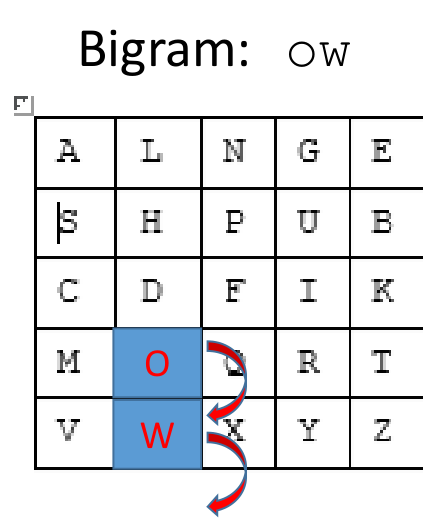
\includegraphics[width=46.20mm,height=142.56mm]{images/llm/page_075_img_02.png}%
\end{textblock*}

\newpage

% --- unit llm 76 ---
% === Halaman 76 (llm) ===

3. Jika dua huruf tidak pada baris yang sama atau kolom yang sama, maka:\
\begin{itemize}
    \item huruf pertama diganti dengan huruf pada perpotongan baris huruf pertama dengan kolom huruf kedua.
    \item huruf kedua diganti dengan huruf pada titik sudut keempat dari persegi panjang yang dibentuk dari tiga huruf yang digunakan sampai sejauh ini.
\end{itemize}

\vspace{10mm}

\begin{center}
    Bigram: hz\\
    \vspace{5mm}
    Cipherteks: BW
\end{center}

% deskripsi: Tabel matriks huruf untuk metode enkripsi Playfair yang menunjukkan proses pencarian ciphertext untuk bigram 'hz', dengan panah merah yang menghubungkan huruf H, B, dan Z untuk membentuk persegi panjang.
% bbox normalisasi: [0.3570, 0.5600, 0.5670, 0.9050]
\begin{textblock*}{44.10mm}(74.97mm,166.32mm)
\noindent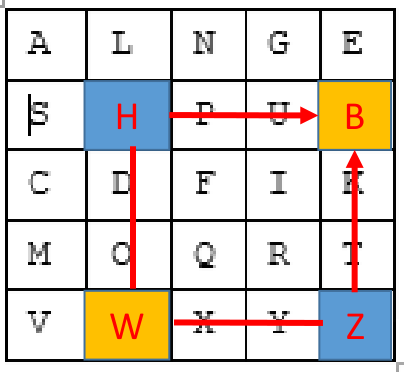
\includegraphics[width=44.10mm,height=102.46mm]{images/llm/page_076_img_01.png}%
\end{textblock*}

\newpage

% --- unit llm 77 ---
% === Halaman 77 (llm) ===

Bigram IH diganti menjadi MB

\vspace{10mm}

Sumber gambar: Wikipedia

% deskripsi: Ilustrasi penggantian bigram IH menjadi MB pada tabel Playfair, menunjukkan pergerakan huruf I ke M dan H ke B menggunakan tanda panah.
% bbox normalisasi: [0.2920, 0.3200, 0.6480, 0.5620]
\begin{textblock*}{74.76mm}(61.32mm,95.04mm)
\noindent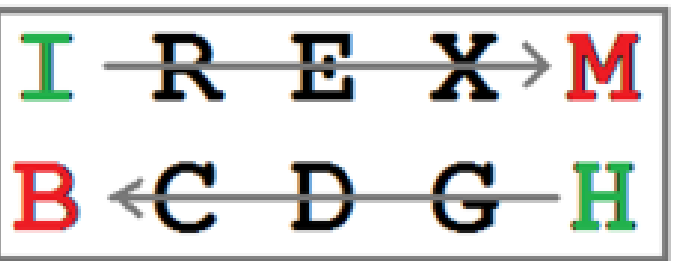
\includegraphics[width=74.76mm,height=71.87mm]{images/llm/page_077_img_01.png}%
\end{textblock*}

\newpage

% --- unit llm 78 ---
% === Halaman 78 (llm) ===

Plainteks: temui ibu nanti malam

Bigram: te mu ix ib un an ti ma la mx

\vspace{10mm}

Kunci: 

\vspace{10mm}

Cipherteks: ZB RS FY KU PG LG RK VS NL QV

% deskripsi: Tabel kunci kriptografi berupa grid 5x5 yang berisi huruf-huruf alfabet (tanpa huruf J) untuk proses enkripsi.
% bbox normalisasi: [0.1970, 0.2770, 0.4200, 0.6400]
\begin{textblock*}{46.83mm}(41.37mm,82.27mm)
\noindent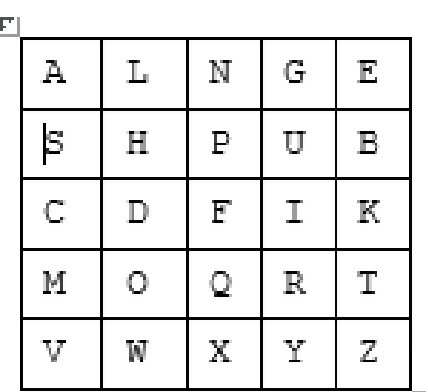
\includegraphics[width=46.83mm,height=107.81mm]{images/llm/page_078_img_01.png}%
\end{textblock*}

\newpage

% --- unit llm 79 ---
% === Halaman 79 (llm) ===

Cara enkripsinya sebagai berikut:

Bigram: \textcolor{red}{te} mu ix ib un an ti ma la mx

\vspace{145.53mm}

Cipherteks: \textcolor{red}{ZB} RS FY KU PG LG RK VS NL QV

\vspace{30mm}

% deskripsi: Ilustrasi proses enkripsi Playfair cipher yang menunjukkan penggunaan tabel 5x5 untuk mencari pasangan huruf, dengan panah yang mengarah ke huruf Z dan B untuk bigram 'te', serta proses pencarian untuk bigram 'mu'.
% bbox normalisasi: [0.1200, 0.4400, 0.8700, 0.9300]
\begin{textblock*}{157.50mm}(25.20mm,130.68mm)
\noindent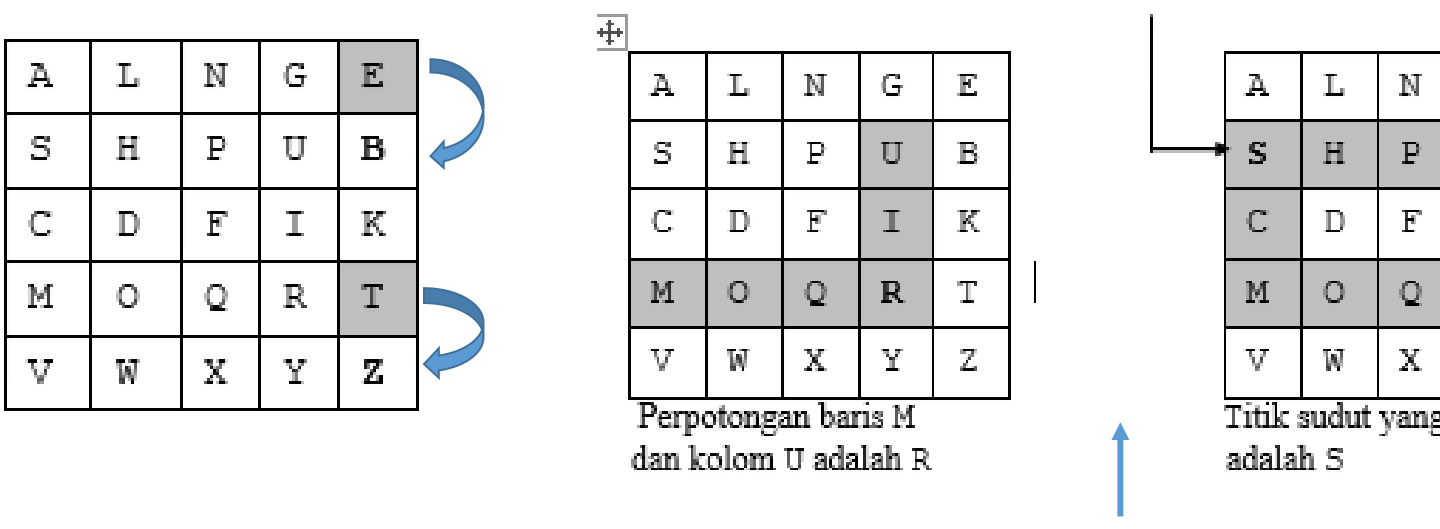
\includegraphics[width=157.50mm,height=145.53mm]{images/llm/page_079_img_01.png}%
\end{textblock*}

\newpage

% --- unit llm 80 ---
% === Halaman 80 (llm) ===

Algoritma dekripsi kebalikan dari algoritma enkripsi. Langkah-langkahnya adalah sebagai berikut:

\begin{enumerate}
  \item Jika dua huruf terdapat pada baris bujursangkar yang sama maka tiap huruf diganti dengan huruf di kirinya.
  \item Jika dua huruf terdapat pada kolom bujursangkar yang sama maka tiap huruf diganti dengan huruf di atasnya.
  \item Jika dua huruf tidak pada baris yang sama atau kolom yang sama, maka huruf pertama diganti dengan huruf pada perpotongan baris huruf pertama dengan kolom huruf kedua. Huruf kedua diganti dengan huruf pada titik sudut keempat dari persegi panjang yang dibentuk dari tiga huruf yang digunakan sampai sejauh ini.
  \item Buanglah huruf X yang tidak mengandung makna.
\end{enumerate}

\newpage

% --- unit llm 81 ---
% === Halaman 81 (llm) ===

\vspace{213.84mm}

Demo Playfair cipher online: \url{https://planetcalc.com/7751/}

% deskripsi: Screenshot alat kalkulator online Playfair cipher yang menunjukkan teks input, keyword, proses enkripsi, kotak Playfair (Playfair square), dan teks hasil transformasi.
% bbox normalisasi: [0.7300, 0.1400, 0.9000, 0.8600]
\begin{textblock*}{35.70mm}(153.30mm,41.58mm)
\noindent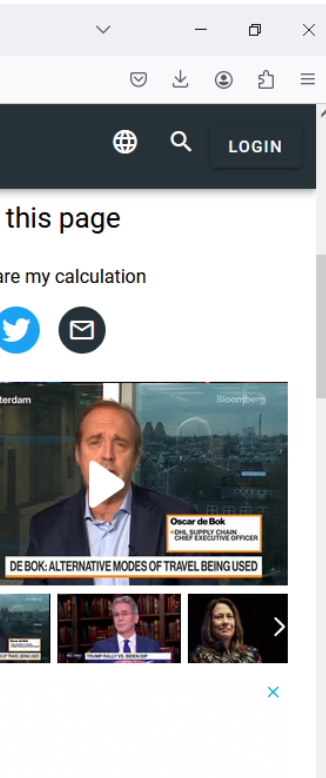
\includegraphics[width=35.70mm,height=213.84mm]{images/llm/page_081_img_01.png}%
\end{textblock*}

\newpage

% --- unit llm 82 ---
% === Halaman 82 (llm) ===

\section*{Kriptanalisis Playfair Cipher}

\begin{itemize}
    \item Karena ada 26 huruf abjad, maka terdapat $26 \times 26 = 677$ bigram, sehingga identifikasi bigram individual lebih sukar.
    \item Sayangnya ukuran poligram di dalam \textit{Playfair cipher} tidak cukup besar, hanya dua huruf sehingga \textit{Playfair cipher} tetap tidak aman.
    \item Meskipun \textit{Playfair cipher} sulit dipecahkan dengan analisis frekuensi relatif huruf-huruf, namun ia dapat dipecahkan dengan analisis frekuensi pasangan huruf.
    \item Dalam Bahasa Inggris kita bisa mempunyai frekuensi kemunculan pasangan huruf, misalnya pasangan huruf TH dan HE paling sering muncul.
\end{itemize}

\newpage

% --- unit llm 83 ---
% === Halaman 83 (llm) ===

% (tidak ada teks dari model)

% deskripsi: Grafik batang yang menunjukkan nilai numerik untuk berbagai kategori yang diberi label dua huruf (AN, AT, ED, EN, ER, ES, HE, IN, ON, OR, RE, ST, TE, TH, TI). Nilai tertinggi adalah TH dengan 3.21 dan terendah adalah ST dengan 1.22.
% bbox normalisasi: [0.1050, 0.1560, 0.9500, 0.7500]
\begin{textblock*}{177.45mm}(22.05mm,46.33mm)
\noindent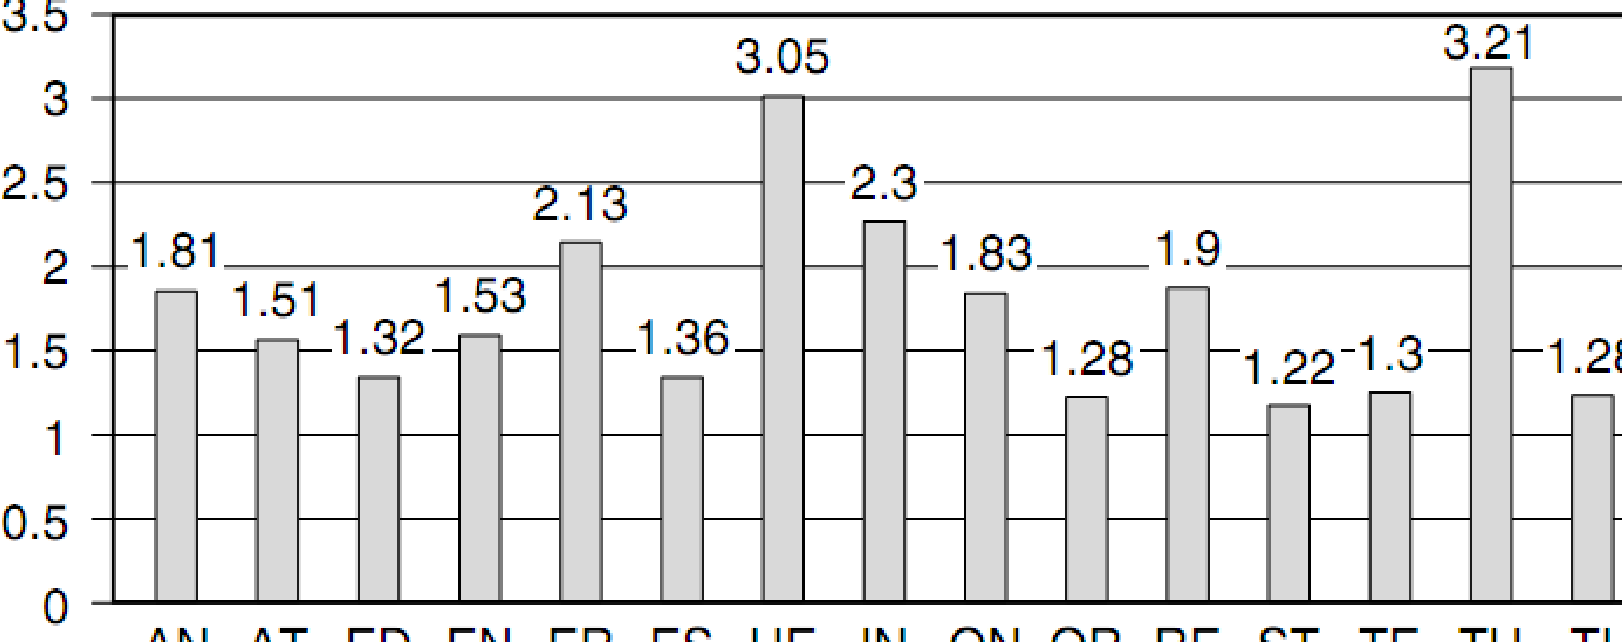
\includegraphics[width=177.45mm,height=176.42mm]{images/llm/page_083_img_01.png}%
\end{textblock*}

\newpage

% --- unit llm 84 ---
% === Halaman 84 (llm) ===

\vspace{279.18mm}

\vspace{10mm}
\begin{itemize}
    \item Dengan menggunakan tabel frekuensi kemunculan pasangan huruf di dalam Bahasa Inggris dan cipherteks yang cukup banyak, \textit{Playfair cipher} dapat dipecahkan.
    \item Kelemahan lainnya, bigram dan kebalikannya (misal AB dan BA) akan didekripsi menjadi pola huruf plainteks yang sama (misal RE dan ER). Di dalam bahasa Inggris terdapat banyak kata yang mengandung bigram terbalik seperti REceivER dan DEpartED.
\end{itemize}

% deskripsi: Grafik batang distribusi bigram yang menunjukkan frekuensi kemunculan pasangan huruf dalam bahasa Inggris, dengan 'TH' sebagai yang paling sering muncul.
% bbox normalisasi: [0.0000, 0.0000, 0.3200, 0.9400]
\begin{textblock*}{67.20mm}(0.00mm,0.00mm)
\noindent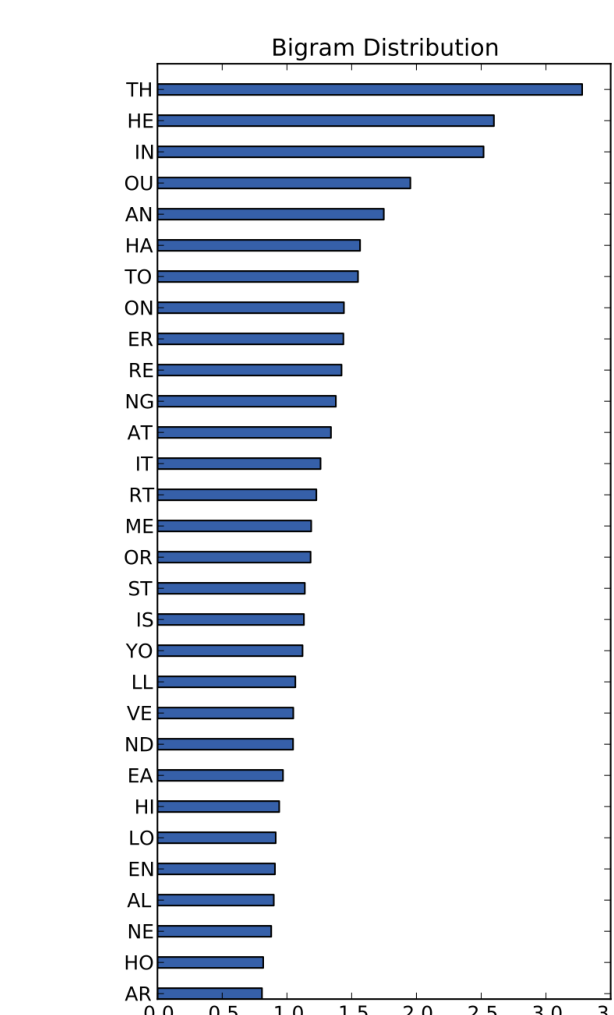
\includegraphics[width=67.20mm,height=279.18mm]{images/llm/page_084_img_01.png}%
\end{textblock*}

\newpage

% --- unit llm 85 ---
% === Halaman 85 (llm) ===

\begin{itemize}
  \item Contoh:
  \begin{itemize}
    \item misalkan bigram yang sering muncul di dalam cipherteks adalah BM.
    \item bigram yang sering muncul di dalam bahasa Inggris adalah TH
    \item jadi, kita duga TH dipetakan menjadi BM
    \item misalkan TH dienkripsi dengan aturan segiempat, maka jika T dan H membentuk segiempat dengan B dan M, maka posisi mereka harus konsisten dalam matriks.
    \item Artinya: T satu baris dengan B, dan H satu baris dengan M
  \end{itemize}
\end{itemize}

\vspace{15mm}

\begin{itemize}
  \item Jika TH dienkripsi dengan aturan kolom, maka B di bawah T, M di bawah H
  \item Jika TH dienkripsi dengan aturan baris, maka B di kanan T, M di kanan H
  \item Mulai bangun matriks parsial $5 \times 5$ dengan hipotesis seperti di atas
\end{itemize}

% deskripsi: Ilustrasi posisi huruf T, B, M, dan H yang membentuk segiempat dalam matriks
% bbox normalisasi: [0.2100, 0.5500, 0.3200, 0.7400]
\begin{textblock*}{23.10mm}(44.10mm,163.35mm)
\noindent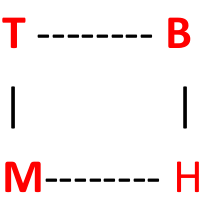
\includegraphics[width=23.10mm,height=56.43mm]{images/llm/page_085_img_01.png}%
\end{textblock*}

\newpage

% --- unit llm 86 ---
% === Halaman 86 (llm) ===

\section*{C. Affine Cipher}

\begin{itemize}
    \item Merupakan perluasan \textit{Caesar cipher}
    
    Enkripsi: \[ C \equiv mP + b \pmod{n} \]
    
    Dekripsi: \[ P \equiv m^{-1} (C - b) \pmod{n} \]
    
    \item Kunci: $m$ dan $b$
\end{itemize}

\textbf{Keterangan:}

\begin{enumerate}
    \item $n$ adalah ukuran alfabet
    \item $m$ bilangan bulat yang relatif prima dengan $n$
    \item $b$ adalah jumlah pergeseran
    \item \textit{Caesar cipher} adalah khusus dari \textit{affine cipher} dengan $m = 1$
    \item $m^{-1}$ adalah inversi $m \pmod{n}$, yaitu $m \cdot m^{-1} \equiv 1 \pmod{n}$
\end{enumerate}

\newpage

% --- unit llm 87 ---
% === Halaman 87 (llm) ===

\begin{itemize}
  \item Contoh:
  \end{itemize}

Plainteks: \texttt{kripto} $(10 \ 17 \ 8 \ 15 \ 19 \ 14)$

$n = 26$, ambil $m = 7$ (7 relatif prima dengan 26)

\vspace{5mm}

Enkripsi: $C \equiv 7P + 10 \pmod{26}$

\begin{align*}
 p_1 = 10 & \to c_1 \equiv 7 \cdot 10 + 10 \equiv 80 \equiv 2 \pmod{26} && (\text{huruf 'C'})
 p_2 = 17 & \to c_2 \equiv 7 \cdot 17 + 10 \equiv 129 \equiv 25 \pmod{26} && (\text{huruf 'Z'})
 p_3 = 8 & \to c_3 \equiv 7 \cdot 8 + 10 \equiv 66 \equiv 14 \pmod{26} && (\text{huruf 'O'})
 p_4 = 15 & \to c_4 \equiv 7 \cdot 15 + 10 \equiv 115 \equiv 11 \pmod{26} && (\text{huruf 'L'})
 p_5 = 19 & \to c_5 \equiv 7 \cdot 19 + 10 \equiv 143 \equiv 13 \pmod{26} && (\text{huruf 'N'})
 p_6 = 14 & \to c_6 \equiv 7 \cdot 14 + 10 \equiv 108 \equiv 4 \pmod{26} && (\text{huruf 'E'})
\end{align*}

\vspace{5mm}

Cipherteks: \texttt{CZOLNE}

\newpage

% --- unit llm 88 ---
% === Halaman 88 (llm) ===

\begin{itemize}
  \item Dekripsi:
  \begin{itemize}
    \item Mula-mula hitung $m^{-1}$ yaitu $7^{-1} \pmod{26}$ dengan memecahkan $7x \equiv 1 \pmod{26}$
    
    Solusinya: $x \equiv 15 \pmod{26}$ sebab $7 \cdot 15 = 105 \equiv 1 \pmod{26}$.
    
    \item Jadi, $P \equiv 15(C - 10) \pmod{26}$
  \end{itemize}
\end{itemize}

\begin{align*}
  c_1 = 2 \quad &\rightarrow p_1 \equiv 15 \cdot (2 - 10) = -120 \equiv 10 \pmod{26} \quad (\text{huruf 'k'})
  c_2 = 25 \quad &\rightarrow p_2 \equiv 15 \cdot (25 - 10) = 225 \equiv 17 \pmod{26} \quad (\text{huruf 'r'})
  c_3 = 14 \quad &\rightarrow p_3 \equiv 15 \cdot (14 - 10) = 60 \equiv 8 \pmod{26} \quad (\text{huruf 'i'})
  c_4 = 11 \quad &\rightarrow p_4 \equiv 15 \cdot (11 - 10) = 15 \equiv 15 \pmod{26} \quad (\text{huruf 'p'})
  c_5 = 13 \quad &\rightarrow p_5 \equiv 15 \cdot (13 - 10) = 45 \equiv 19 \pmod{26} \quad (\text{huruf 't'})
  c_6 = 4 \quad &\rightarrow p_6 \equiv 15 \cdot (4 - 10) = -90 \equiv 14 \pmod{26} \quad (\text{huruf 'o'})
\end{align*}

Plainteks yang diungkap kembali: \texttt{kripto}

\newpage

% --- unit llm 89 ---
% === Halaman 89 (llm) ===

\vspace{207.90mm}

Demo affine cipher online: \url{https://cryptii.com/pipes/affine-cipher}

\vspace{10mm}

Affine cipher: Encode and decode

% deskripsi: Screenshot antarmuka situs web Cryptii yang menunjukkan proses enkripsi Affine Cipher dengan plaintext 'Pinjam dulu seratus' menjadi ciphertext 'Gxwcwjryfmvdqjafv' menggunakan parameter Slope/A = 5 dan Intercept/B = 9.
% bbox normalisasi: [0.8000, 0.1400, 0.9400, 0.8400]
\begin{textblock*}{29.40mm}(168.00mm,41.58mm)
\noindent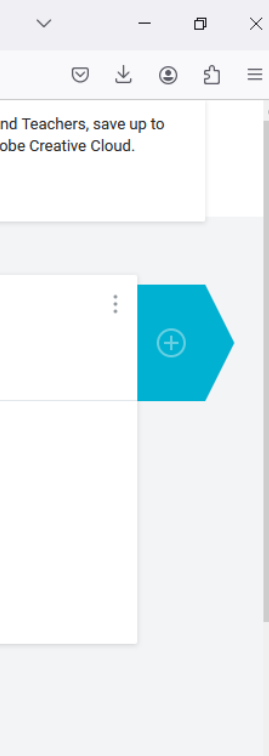
\includegraphics[width=29.40mm,height=207.90mm]{images/llm/page_089_img_01.png}%
\end{textblock*}

\newpage

% --- unit llm 90 ---
% === Halaman 90 (llm) ===

\section*{Kriptanalisis Affine Cipher}

\begin{itemize}
    \item Affine Cipher:
    \[ \text{Enkripsi: } C \equiv mP + b \pmod{n} \]
    \[ \text{Dekripsi: } P \equiv m^{-1} (C - b) \pmod{n} \]
    
    \item Affine cipher mudah diserang dengan \textit{known-plaintext attack} (sebagian plainteks dari pesan diketahui)
    
    \item Misalkan kriptanalis mempunyai dua buah plainteks, $P_1$ dan $P_2$, yang berkoresponden dengan cipherteks $C_1$ dan $C_2$,
    
    \item maka $m$ dan $b$ mudah dihitung dari buah kekongruenan simultan berikut ini:
    \begin{align*}
        C_1 &\equiv mP_1 + b \pmod{n} \\
        C_2 &\equiv mP_2 + b \pmod{n}
    \end{align*}
\end{itemize}

\newpage

% --- unit llm 91 ---
% === Halaman 91 (llm) ===

\begin{itemize}
    \item Contoh: Misalkan kriptanalis menemukan
    \begin{center}
        cipherteks $\text{C}$ dan plainteks berkorepsonden $\text{K}$ \\
        cipherteks $\text{E}$ dan plainteks berkorepsonden $\text{O}$.
    \end{center}

    \item Kriptanalis $m$ dan $n$ dari kekongruenan berikut:
    \begin{align}
        2 &\equiv 10m + b \pmod{26} && (\text{i}) \\
        4 &\equiv 14m + b \pmod{26} && (\text{ii})
    \end{align}

    \item Kurangkan (ii) dengan (i), menghasilkan
    \begin{align}
        2 &\equiv 4m \pmod{26} && (\text{iii}) \\
        \text{Solusi: } & m = 7
    \end{align}

    Substitusi $m = 7$ ke dalam (i),
    \begin{align}
        2 &\equiv 70 + b \pmod{26} && (\text{iv}) \\
        \text{Solusi: } & b = 10.
    \end{align}
\end{itemize}

\newpage

% --- unit llm 92 ---
% === Halaman 92 (llm) ===

\begin{itemize}
    \item Jika pasangan plainteks dan cipherteks tidak tersedia, maka Affine Cipher masih bisa diserang dengan \textit{exhaustive key search}.
    \item sebab ada 25 pilihan untuk $b$ dan 12 buah nilai $m$ yang relatif prima dengan 26 (yaitu 1, 3, 5, 7, 9, 11, 15, 17, 19, 21, 23, dan 25).
    \item Dengan mencoba sebanyak $25 \times 12 = 300$ susunan $b$ dan $m$, maka nilai $b$ dan $m$ yang benar dapat ditemukan dengan mudah, karena 300 susunan $b$ dan $m$ adalah jumlah yang sangat sedikit.
\end{itemize}

\newpage

% --- unit llm 93 ---
% === Halaman 93 (llm) ===

\begin{itemize}
    \item Salah satu cara memperbesar faktor kerja untuk \textit{exhaustive key search}: adalah dengan cara enkripsi tidak dilakukan terhadap huruf individual, tetapi dalam blok huruf.
    \item Misal, pesan \texttt{kriptografi} dipecah menjadi kelompok 4-huruf:
    \[ \texttt{krip togr afi} \]
\end{itemize}

(ekivalen dengan 10170815 19140617 000508, dengan memisalkan 'A' = 0, 'B' = 1, ..., 'Z' = 25)

\newpage

% --- unit llm 94 ---
% === Halaman 94 (llm) ===

\begin{itemize}
    \item Nilai terbesar yang dapat muncul untuk merepresentasikan blok: $25252525$ (ZZZZ), maka $25252525$ dapat digunakan sebagai modulus $n$.
    \item Nilai $m$ yang relatif prima dengan $25252525$, misalnya $21035433$,
    \item $b$ dipilih antara $1$ dan $25252525$, misalnya $23210025$.
\end{itemize}

\noindent Fungsi enkripsi menjadi:
\[ C \equiv 21035433P + 23210025 \pmod{25252525} \]

\noindent Fungsi dekripsi, setelah dihitung, menjadi
\[ P \equiv 5174971 (C - 23210025) \pmod{25252525} \]

\newpage

% --- unit llm 95 ---
% === Halaman 95 (llm) ===

\section*{D. Hill Cipher}

\begin{itemize}
    \item Dikembangkan oleh Lester Hill (1929), termasuk ke dalam polygram cipher yang berbasis aljabar linier
    \item Menggunakan $m$ buah persamaan linier
    \item Untuk $m = 3$ (enkripsi setiap 3 huruf), sistem persamaan linernya menjadi:
\end{itemize}

\vspace{10mm}

\begin{align*}
C_1 &= (k_{11} p_1 + k_{12} p_2 + k_{13} p_3) \pmod{26} \\
C_2 &= (k_{21} p_1 + k_{22} p_2 + k_{23} p_3) \pmod{26} \\
C_3 &= (k_{31} p_1 + k_{32} p_2 + k_{33} p_3) \pmod{26}
\end{align*}

\vspace{10mm}

\[ \mathbf{C} = \mathbf{KP} \]

% deskripsi: Representasi matriks dari sistem persamaan linier Hill Cipher untuk m=3
% bbox normalisasi: [0.5140, 0.5420, 0.9300, 0.7830]
\begin{textblock*}{87.36mm}(107.94mm,160.97mm)
\noindent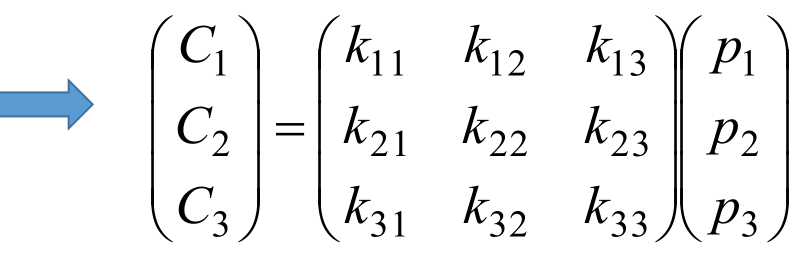
\includegraphics[width=87.36mm,height=71.58mm]{images/llm/page_095_img_01.png}%
\end{textblock*}

\newpage

% --- unit llm 96 ---
% === Halaman 96 (llm) ===

\section*{Lester S. Hill}

\vspace{198.99mm}

From Wikipedia, the free encyclopedia

\textbf{Lester S. Hill} (1891--1961) was an American mathematician and educator who was interested in applications of mathematics to communications. He received a bachelor's degree (1911) and a master's degree (1913) from Columbia College and a Ph.D. from Yale University (1926). He taught at the University of Montana, Princeton University, the University of Maine, Yale University, and Hunter College. Among his notable contributions was the Hill cipher. He also developed methods for detecting errors in telegraphed code numbers and wrote two books.

\vspace{20mm}

\subsection*{References}

\begin{enumerate}
    \item $\wedge$ Christensen, Chris (2014). "Lester Hill Revisited". \textit{Cryptologia}. 38 (4): 300--301. doi:10.1080/01611194.2014.915260. S2CID 45603857. Retrieved November 9, 2018 -- via ResearchGate.
    \item $\wedge$ a b "Dr. Lester S. Hill", \textit{Chicago Tribune}, January 10, 1961. p. 10. "Dr. Lester S. Hill, 70, mathematician and cryptographer, died today in Lawrence hospital after a long illness. Hill was commended for application, of higher mathematics to the construction of secret codes."
\end{enumerate}

% deskripsi: Infobox Wikipedia mengenai profil Dr. Lester S. Hill yang berisi foto, tanggal lahir, tanggal wafat, pekerjaan, dan karya terkenal.
% bbox normalisasi: [0.5700, 0.2200, 0.8200, 0.8900]
\begin{textblock*}{52.50mm}(119.70mm,65.34mm)
\noindent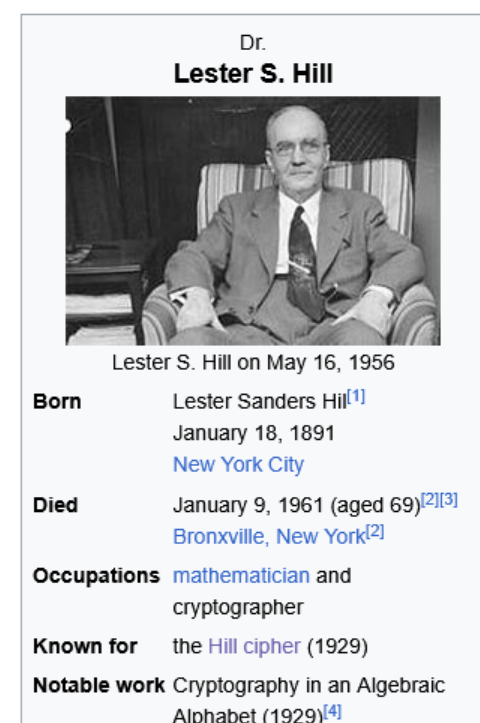
\includegraphics[width=52.50mm,height=198.99mm]{images/llm/page_096_img_01.png}%
\end{textblock*}

\newpage

% --- unit llm 97 ---
% === Halaman 97 (llm) ===

\begin{itemize}
  \item Contoh:
\end{itemize}

\vspace{10mm}

\[ K = \begin{pmatrix} 17 & 17 & 5 \\ 21 & 18 & 21 \\ 2 & 2 & 19 \end{pmatrix} \]

Plainteks: \texttt{paymoremoney} \\
Enkripsi tiga huruf pertama: $\text{pay} = (15, 0, 24)$

\vspace{10mm}

\[ C = \begin{pmatrix} 17 & 17 & 5 \\ 21 & 18 & 21 \\ 2 & 2 & 19 \end{pmatrix} \begin{pmatrix} 15 \\ 0 \\ 24 \end{pmatrix} = \begin{pmatrix} 375 \\ 819 \\ 486 \end{pmatrix} \pmod{26} = \begin{pmatrix} 11 \\ 13 \\ 18 \end{pmatrix} = \text{LNS} \]

Cipherteks selengkapnya: \texttt{LNSHDLEWMTRW}

% deskripsi: Tabel pemetaan huruf alfabet A-Z ke angka 0-25
% bbox normalisasi: [0.0600, 0.1080, 0.9400, 0.9120]
\begin{textblock*}{184.80mm}(12.60mm,32.08mm)
\noindent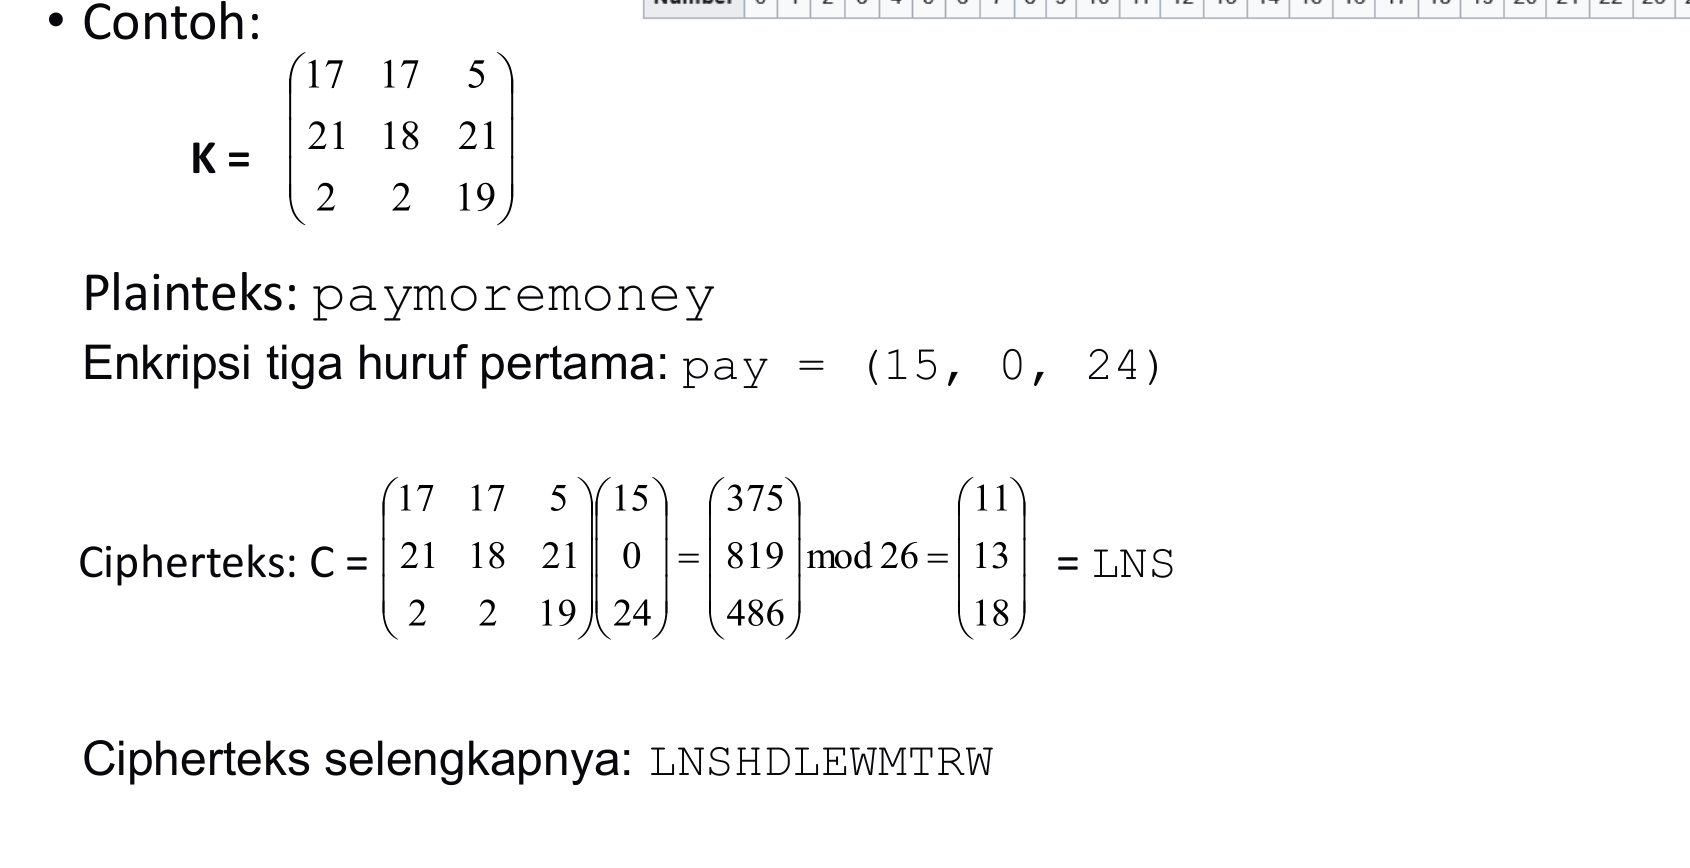
\includegraphics[width=184.80mm,height=238.79mm]{images/llm/page_097_img_01.png}%
\end{textblock*}

% bbox perkiraan otomatis: Tabel pemetaan huruf alfabet A-Z ke angka 0-25

\newpage

% --- unit llm 98 ---
% === Halaman 98 (llm) ===

\begin{itemize}
  \item Dekripsi perlu menghitung $\mathbf{K}^{-1}$ sedemikian sehingga $\mathbf{KK}^{-1} = \mathbf{I}$ ($\mathbf{I}$ matriks identitas).
\end{itemize}

\vspace{10mm}

sebaba

% deskripsi: Persamaan matriks untuk menentukan invers matriks K
% bbox normalisasi: [0.1200, 0.2500, 0.7800, 0.4300]
\begin{textblock*}{138.60mm}(25.20mm,74.25mm)
\noindent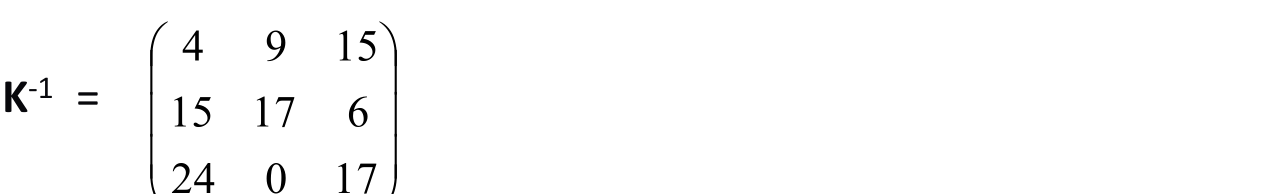
\includegraphics[width=138.60mm,height=53.46mm]{images/llm/page_098_img_01.png}%
\end{textblock*}

% deskripsi: Perhitungan perkalian matriks modulo 26 untuk membuktikan hasil invers
% bbox normalisasi: [0.1300, 0.5800, 0.7700, 0.7600]
\begin{textblock*}{134.40mm}(27.30mm,172.26mm)
\noindent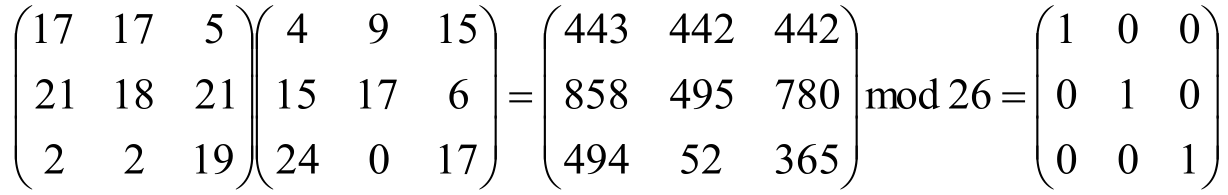
\includegraphics[width=134.40mm,height=53.46mm]{images/llm/page_098_img_02.png}%
\end{textblock*}

\newpage

% --- unit llm 99 ---
% === Halaman 99 (llm) ===

\begin{itemize}
  \item Cara menghitung matriks invers $2 \times 2$:
\end{itemize}

\vspace{20mm}

Contoh: $K = \begin{pmatrix} 3 & 10 \\ 15 & 9 \end{pmatrix}$

\[ \det(K) = (3)(9) - (15)(10) = 27 - 150 = -123 \pmod{26} = 7 \]

% deskripsi: Rumus umum invers matriks 2x2
% bbox normalisasi: [0.1100, 0.2070, 0.6480, 0.5530]
\begin{textblock*}{112.98mm}(23.10mm,61.48mm)
\noindent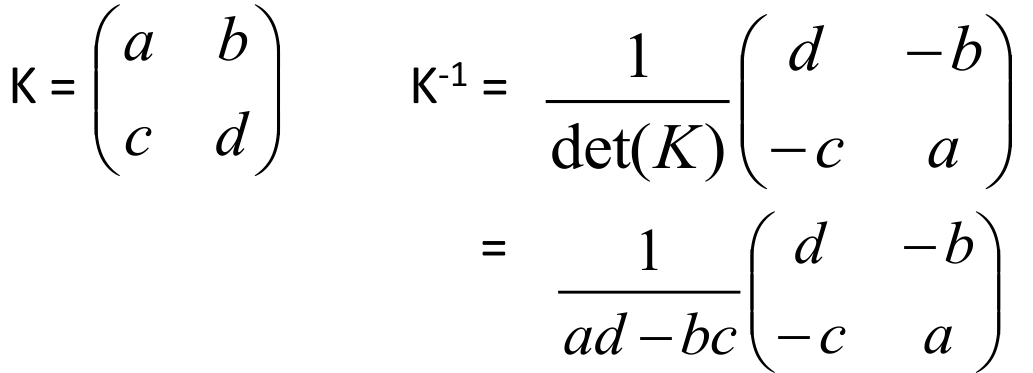
\includegraphics[width=112.98mm,height=102.76mm]{images/llm/page_099_img_01.png}%
\end{textblock*}

\newpage

% --- unit llm 100 ---
% === Halaman 100 (llm) ===

\begin{align*}
K^{-1} &= \frac{1}{7} \begin{pmatrix} 3 & 10 \\ 15 & 9 \end{pmatrix} = 7^{-1} \begin{pmatrix} 9 & -10 \\ -15 & 3 \end{pmatrix} \\ &= 15 \begin{pmatrix} 9 & -10 \\ -15 & 3 \end{pmatrix} = 15 \begin{pmatrix} 9 & 16 \\ 11 & 3 \end{pmatrix} = \begin{pmatrix} 135 & 240 \\ 165 & 45 \end{pmatrix} \pmod{26} = \begin{pmatrix} 5 & 6 \\ 9 & 19 \end{pmatrix}
\end{align*}

\vspace{10mm}

\textbf{Keterangan} (ingat kembali teori bilangan di dalam Matematika Diskrit):
\begin{enumerate}[(i)]
\item $7^{-1} \pmod{26} \equiv 15$, karena $(7)(15) = 105 \pmod{26} = 1$
\item $-10 \equiv 16 \pmod{26}$
\item $-15 \equiv 11 \pmod{26}$ 
\end{enumerate}

\newpage

% --- unit llm 101 ---
% === Halaman 101 (llm) ===

Periksa bahwa:

\begin{align*}
\mathbf{KK}^{-1} &= \begin{pmatrix} 3 & 10 \\ 15 & 9 \end{pmatrix} \begin{pmatrix} 5 & 6 \\ 9 & 19 \end{pmatrix} = \begin{pmatrix} 3\cdot 5 + 10\cdot 9 & 3\cdot 6 + 10\cdot 19 \\ 15\cdot 5 + 9\cdot 9 & 15\cdot 6 + 9\cdot 19 \end{pmatrix} \\ &= \begin{pmatrix} 105 & 208 \\ 156 & 261 \end{pmatrix} \pmod{26} = \begin{pmatrix} 1 & 0 \\ 0 & 1 \end{pmatrix}
\end{align*}

\newpage

% --- unit llm 102 ---
% === Halaman 102 (llm) ===

\begin{itemize}
    \item Untuk matriks $3 \times 3$, matriks dapat dicari dengan metode Eliminasi Gauss-Jordan, atau dihitung langsung dengan rumus berikut::
\end{itemize}

\vspace{10mm}

\begin{itemize}
    \item yang dalam hal ini,
\end{itemize}

\begin{align*}
 A &= (ei - hf) & B &= -(di - fg) & C &= (dh - eg) \\
 D &= -(bi - hc) & E &= (ai - cg) & F &= -(ah - bg) \\
 G &= (bf - ec) & H &= -(af - cd) & I &= (ae - bd)
\end{align*}

dan

\[ 
\det(\mathbf{K}) = aA + bB + cC
\]

% deskripsi: Rumus perhitungan invers matriks 3x3 menggunakan determinan dan matriks kofaktor yang ditranspose.
% bbox normalisasi: [0.1800, 0.2300, 0.7700, 0.3900]
\begin{textblock*}{123.90mm}(37.80mm,68.31mm)
\noindent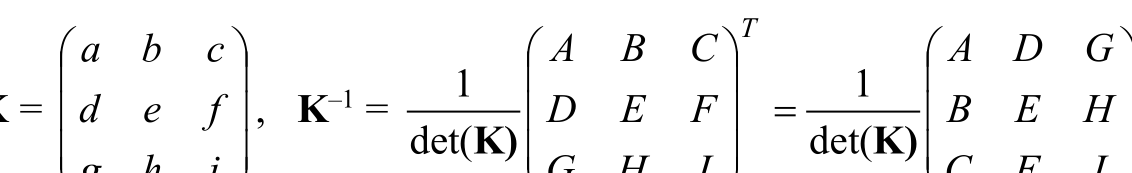
\includegraphics[width=123.90mm,height=47.52mm]{images/llm/page_102_img_01.png}%
\end{textblock*}

\newpage

% --- unit llm 103 ---
% === Halaman 103 (llm) ===

\begin{itemize}
    \item Dekripsi:
\end{itemize}

\[ P = K^{-1} C \]

Cipherteks: $\text{LNS}$ atau $\text{C} = (11, 13, 18)$

\vspace{10mm}

Plainteks: $\begin{pmatrix} 4 & 9 & 15 \\ 15 & 17 & 6 \\ 24 & 0 & 17 \end{pmatrix} \begin{pmatrix} 11 \\ 13 \\ 18 \end{pmatrix} = \begin{pmatrix} 431 \\ 494 \\ 570 \end{pmatrix} \pmod{26} = \begin{pmatrix} 15 \\ 0 \\ 24 \end{pmatrix}$

\vspace{10mm}

$\text{C} = (15, 0, 24) = (\text{P, A, Y})$

% deskripsi: Perhitungan matriks dekripsi Hill Cipher dari cipherteks ke plainteks
% bbox normalisasi: [0.2550, 0.5220, 0.7470, 0.7410]
\begin{textblock*}{103.32mm}(53.55mm,155.03mm)
\noindent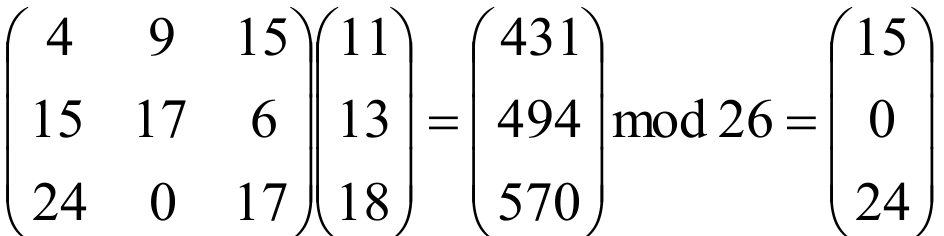
\includegraphics[width=103.32mm,height=65.04mm]{images/llm/page_103_img_01.png}%
\end{textblock*}

\newpage

% --- unit llm 104 ---
% === Halaman 104 (llm) ===

\begin{itemize}
    \item Kekuatan Hill cipher terletak pada penyembunyian frekuensi huruf tunggal
    \item Huruf plainteks yang sama belum tentu dienkripsi menjadi huruf cipherteks yang sama.
\end{itemize}

\newpage

% --- unit llm 105 ---
% === Halaman 105 (llm) ===

\vspace{243.54mm}

Demo Hill Cipher online: https://www.dcode.fr/hill-cipher

% deskripsi: Screenshot antarmuka situs dCode untuk alat Hill Cipher, menunjukkan input ciphertext, matriks kunci 2x2, opsi alfabet, dan area hasil enkripsi/dekripsi.
% bbox normalisasi: [0.6700, 0.1400, 0.9400, 0.9600]
\begin{textblock*}{56.70mm}(140.70mm,41.58mm)
\noindent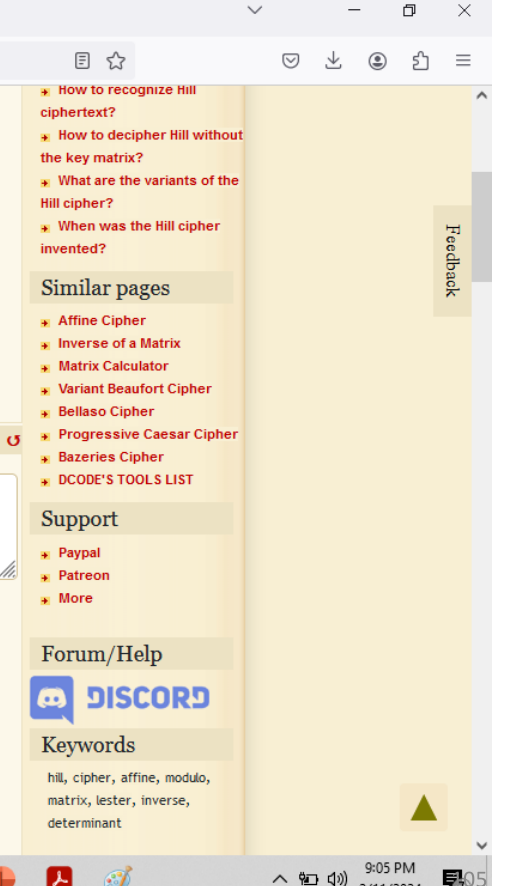
\includegraphics[width=56.70mm,height=243.54mm]{images/llm/page_105_img_01.png}%
\end{textblock*}

\newpage

% --- unit llm 106 ---
% === Halaman 106 (llm) ===

\section*{HILL CIPHER}
Cryptography $\cdot$ Poly-Alphabetic Cipher $\cdot$ Hill Cipher

\vspace{10mm}

\subsection*{HILL DECODER}

\textbf{CIPHERTEXT}

\vspace{151.47mm}

\begin{center}
\begin{tabular}{|c|c|}
\hline
17 & 17 \\ $\hline$
21 & 18 \\ $\hline$
2 & 2 \\ $\hline$
\end{tabular}
\end{center}

$\begin{aligned}
& \text{Try / Bruteforce all } 2\times2 \text{ matrix (values } 10 \le \text{ Latin Alphabet)}
& \text{I know the NON matrix numbers / values}
\end{aligned}$

$\begin{aligned}
& \text{Alphabet options:}
& \square \text{ ALPHABET (26 LET. A=0) ABCDEFGHIJKLMNOPQRSTUVWXYZ}
& \square \text{ ALPHABET (26 LET. A=1) ABCDEFGHIJKLMNOPQRSTUVWXYZ}
& \square \text{ ALPHABET (27 CHAR. A=0) ABCDEFGHIJKLMNOPQRSTUVWXYZ\_}
& \square \text{ ALPHABET (27 CHAR. A=1) \_ABCDEFGHIJKLMNOPQRSTUVWXYZ}
& \square \text{ CUSTOM ALPHANUMERIC ALPHABET}
\end{aligned}$

\vspace{5mm}

\subsection*{Summary}
\begin{itemize}
    \item Hill Decoder
    \item Hill Encoder
    \item Matrix Inversion
    \item What is the Hill cipher? (Definitions)
    \item How to encrypt using Hill cipher?
    \item How to decrypt Hill cipher?
    \item Why must the determinant of the Hill matrix be coprime with 26?
    \item How to decipher Hill without the key matrix?
    \item What are the variants of the Hill cipher?
    \item When was the Hill cipher invented?
\end{itemize}

\subsection*{Similar pages}
\begin{itemize}
    \item Affine Cipher
    \item Inverse of a Matrix
    \item Matrix Calculator
    \item Variant Beaufort Cipher
    \item Bellaso Cipher
\end{itemize}

% deskripsi: Screenshot antarmuka alat Hill Decoder dari situs dCode, menampilkan input teks cipher dan parameter matrix.
% bbox normalisasi: [0.3900, 0.4100, 0.6100, 0.9200]
\begin{textblock*}{46.20mm}(81.90mm,121.77mm)
\noindent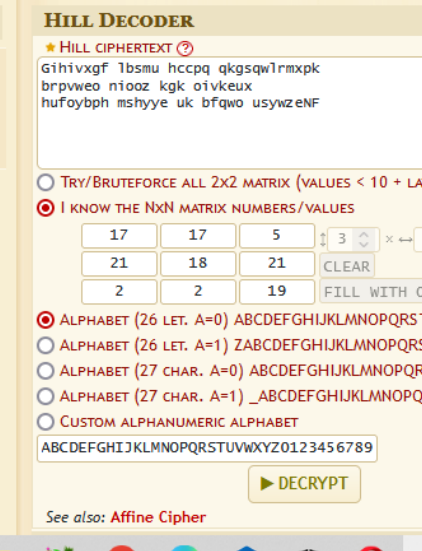
\includegraphics[width=46.20mm,height=151.47mm]{images/llm/page_106_img_01.png}%
\end{textblock*}

\newpage

% --- unit llm 107 ---
% === Halaman 107 (llm) ===

\section*{Kriptanalisis Hill Cipher}

\begin{flushright}
Enkripsi: $\mathrm{C} = \mathrm{KP} \pmod{26}$ \\
Dekripsi: $\mathrm{P} = \mathrm{K}^{-1}\mathrm{C} \pmod{26}$
\end{flushright}

\begin{itemize}
    \item \textit{Hill cipher} mudah dipecahkan dengan \textit{known-plaintext attack}.
    \item Misalkan untuk \textit{Hill cipher} dengan $m = 2$ diketahui:
    \begin{itemize}
        \item $\mathrm{P} = (19, 7) \rightarrow \mathrm{C} = (0, 23)$
        \item $\mathrm{P} = (4, 17) \rightarrow \mathrm{C} = (12, 6)$
        \item Jadi, $\mathrm{K}(19, 7) = (0, 23)$ dan $\mathrm{K}(4, 17) = (12, 6)$
    \end{itemize}
\end{itemize}

\vspace{10mm}

\begin{itemize}
    \item Matriks balikan dari $\mathrm{P}$ adalah $\mathrm{P}^{-1} = \begin{pmatrix} 19 & 4 \\ 7 & 17 \end{pmatrix}^{-1} \pmod{26} = \begin{pmatrix} 25 & 14 \\ 5 & 5 \end{pmatrix}$
    \item Sehingga

    \[ \mathrm{K} = \mathrm{CP}^{-1} \pmod{26} = \begin{pmatrix} 0 & 12 \\ 23 & 6 \end{pmatrix} \begin{pmatrix} 25 & 14 \\ 5 & 5 \end{pmatrix} \pmod{26} = \begin{pmatrix} 8 & 8 \\ 7 & 14 \end{pmatrix} \]
\end{itemize}

% deskripsi: Persamaan matriks untuk mencari kunci K menggunakan known-plaintext attack pada Hill Cipher, menunjukkan hubungan antara matriks C, K, dan P.
% bbox normalisasi: [0.1800, 0.5000, 0.6700, 0.6600]
\begin{textblock*}{102.90mm}(37.80mm,148.50mm)
\noindent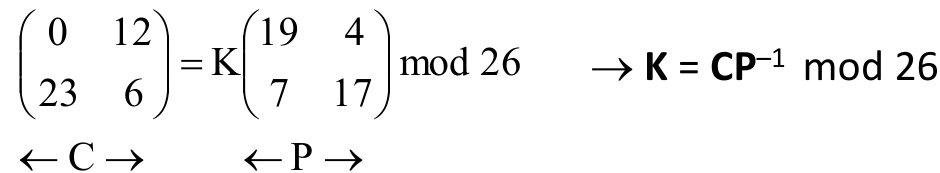
\includegraphics[width=102.90mm,height=47.52mm]{images/llm/page_107_img_01.png}%
\end{textblock*}

\newpage

% --- unit llm 108 ---
% === Halaman 108 (llm) ===

\vspace{242.05mm}

\section*{E. Enigma Cipher}

\begin{itemize}
    \item Enigma adalah mesin enkripsi elektromekanik untuk melakukan enkripsi dan dekripsi.
    \item Ditemukan dan dipatenkan oleh insinyur Jerman, Arthur Scherbius, untuk tujuan komersil, diplomatik, dan militer
    \item Menjadi terkenal karena digunakan oleh tantara Nazi Jerman selama Perang Dunia II untuk mengenkripsi/dekripsi pesan-pesan militer.
    \item Enigma berasal dari bahasa latin, \textit{enigmae}, yang artinya teka-teki.
\end{itemize}

% deskripsi: Foto mesin Enigma dengan label keterangan bagian-bagiannya seperti Rotors, Keyboard, Lampboard, dan Plugboard.
% bbox normalisasi: [0.5760, 0.0700, 0.9370, 0.8850]
\begin{textblock*}{75.81mm}(120.96mm,20.79mm)
\noindent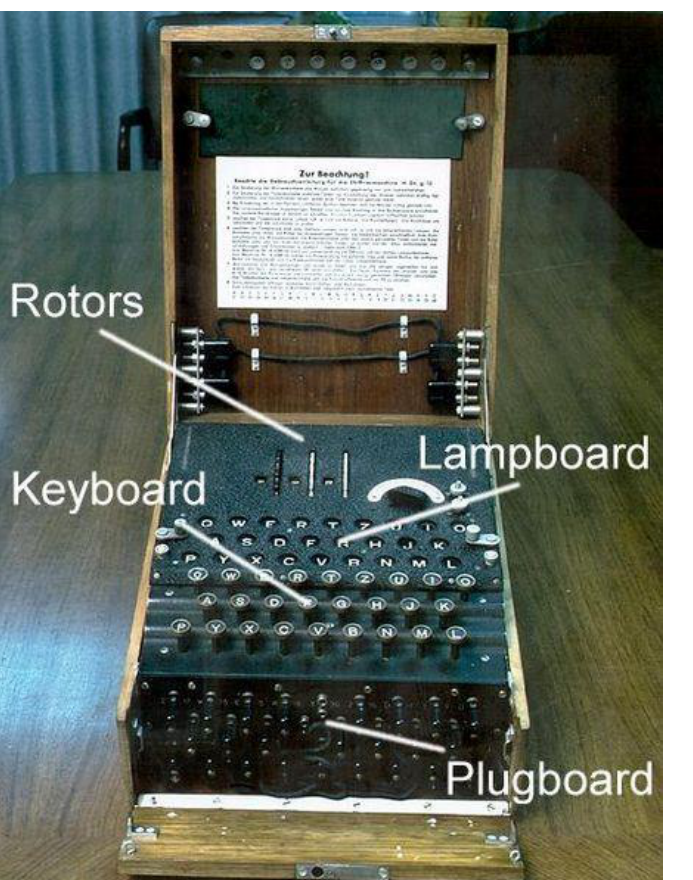
\includegraphics[width=75.81mm,height=242.05mm]{images/llm/page_108_img_01.png}%
\end{textblock*}

\newpage

% --- unit llm 109 ---
% === Halaman 109 (llm) ===

\vspace{95.04mm}

\section*{Enigma Rotors}

\vspace{10mm}

\begin{itemize}
    \item SPARE LIGHT BULBS
    \item VIEWING WINDOWS ON LID SHOW ENCODED LETTERS
    \item ROTOR CYLINDER CARRIES THREE AND LATER FOUR SCRAMBLER ROTORS
    \item POSITION OF ROTORS CONTROLS ENCODING OF EACH LETTER
    \item PLUGBOARD SETTINGS ARE CHANGED DAILY
    \item WOODEN CASE LID
    \item ALPHABETICAL LIGHTBOARD SHOWS FINAL ENCODED LETTERS
    \item KEYBOARD TO TYPE IN MESSAGE
\end{itemize}

% deskripsi: Foto mesin Enigma lengkap dengan label keterangan bagian-bagian utamanya seperti lampu, rotor, keyboard, dan plugboard.
% bbox normalisasi: [0.0200, 0.0000, 0.4300, 0.9800]
\begin{textblock*}{86.10mm}(4.20mm,0.00mm)
\noindent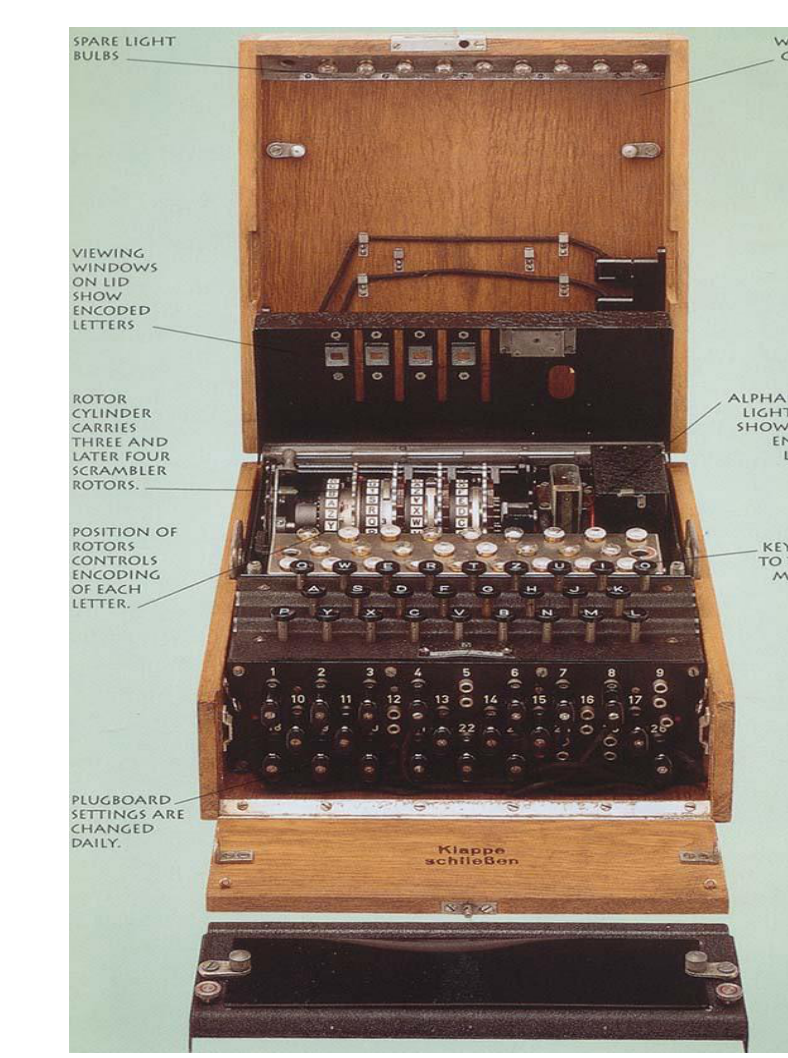
\includegraphics[width=86.10mm,height=291.06mm]{images/llm/page_109_img_01.png}%
\end{textblock*}

% deskripsi: Foto close-up bagian atas satu unit rotor Enigma yang menunjukkan kontak elektrik dan struktur gear.
% bbox normalisasi: [0.6000, 0.1100, 0.8300, 0.4300]
\begin{textblock*}{48.30mm}(126.00mm,32.67mm)
\noindent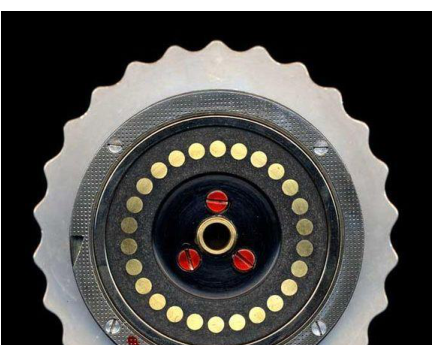
\includegraphics[width=48.30mm,height=95.04mm]{images/llm/page_109_img_02.png}%
\end{textblock*}

% deskripsi: Ilustrasi 3D dari rangkaian rotor Enigma yang menunjukkan susunan cakram alfabet dan poros penggeraknya.
% bbox normalisasi: [0.5900, 0.4600, 0.8500, 0.8500]
\begin{textblock*}{54.60mm}(123.90mm,136.62mm)
\noindent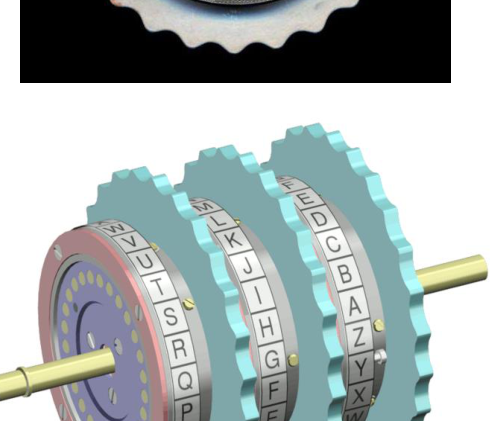
\includegraphics[width=54.60mm,height=115.83mm]{images/llm/page_109_img_03.png}%
\end{textblock*}

\newpage

% --- unit llm 110 ---
% === Halaman 110 (llm) ===

\vspace{136.62mm}

Sumber gambar: https://www.101computing.net/enigma/enigma-instructions.html
\vspace{10mm}
Operator mengetik huruf plainteks pada keyboard, lalu menyalin ulang huruf cipherteks yang menyala pada \textit{lampboard}. Cipherteks dikirim ke penerima pesan

% deskripsi: Ilustrasi simulasi mesin Enigma yang menunjukkan komponen Lampboard, Rotors, Keyboard, dan Plugboard beserta penjelasannya.
% bbox normalisasi: [0.1200, 0.2200, 0.8700, 0.6800]
\begin{textblock*}{157.50mm}(25.20mm,65.34mm)
\noindent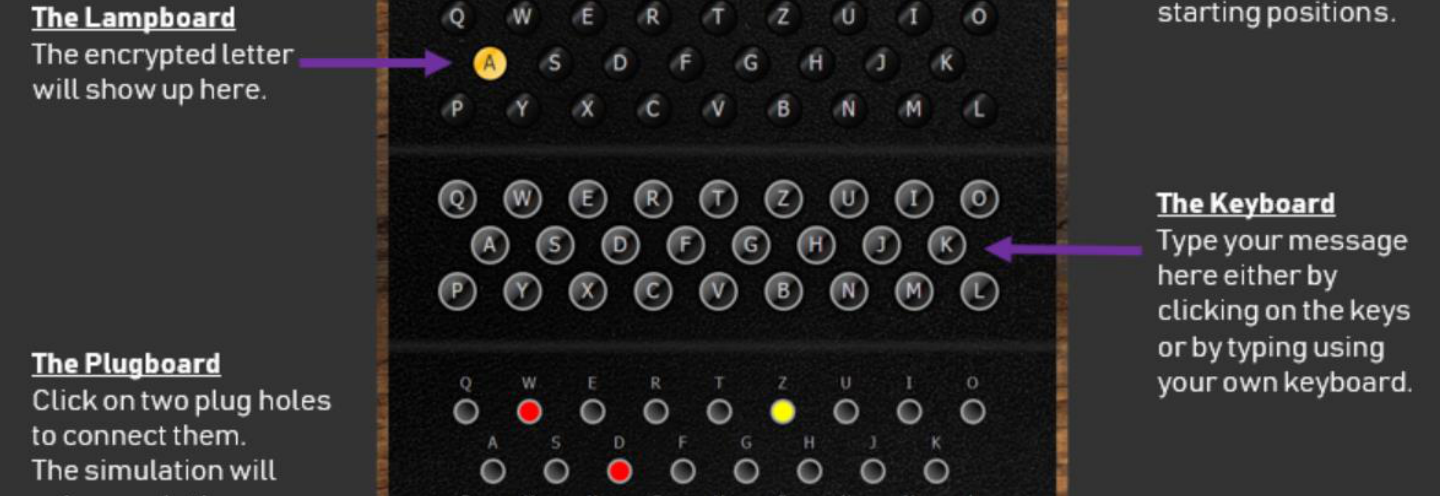
\includegraphics[width=157.50mm,height=136.62mm]{images/llm/page_110_img_01.png}%
\end{textblock*}

\newpage

% --- unit llm 111 ---
% === Halaman 111 (llm) ===

\vspace{162.16mm}

\begin{itemize}
    \item Enigma menggunakan sistem rotor (roda berputar) untuk membentuk huruf cipherteks yang berubah-ubah.
    \item Setiap rotor melakukan substitusi abjad-tunggal (monoalphabetic cipher).
    \item Hasil substitusi oleh suatu rotor menjadi huruf input untuk operasi substitusi rotor selanjutnya.
    \item Hasil substitusi oleh rotor terakhir menjadi huruf cipherteks.
    \item Setiap kali sebuah huruf dienkripsi oleh sebuah rotor, rotor berputar satu huruf untuk membentuk huruf cipherteks baru bagi huruf plainteks berikutnya.
\end{itemize}

\vspace{20mm}

\begin{itemize}
    \item Setelah berputar 26 huruf rotor kembali pada posisi semula. Jadi, diperoleh cipher abjad-majemuk dengan periode 26.
\end{itemize}

% deskripsi: Foto detail mesin Enigma yang memperlihatkan rotor dan papan keyboard huruf.
% bbox normalisasi: [0.5170, 0.1410, 0.9680, 0.6870]
\begin{textblock*}{94.71mm}(108.57mm,41.88mm)
\noindent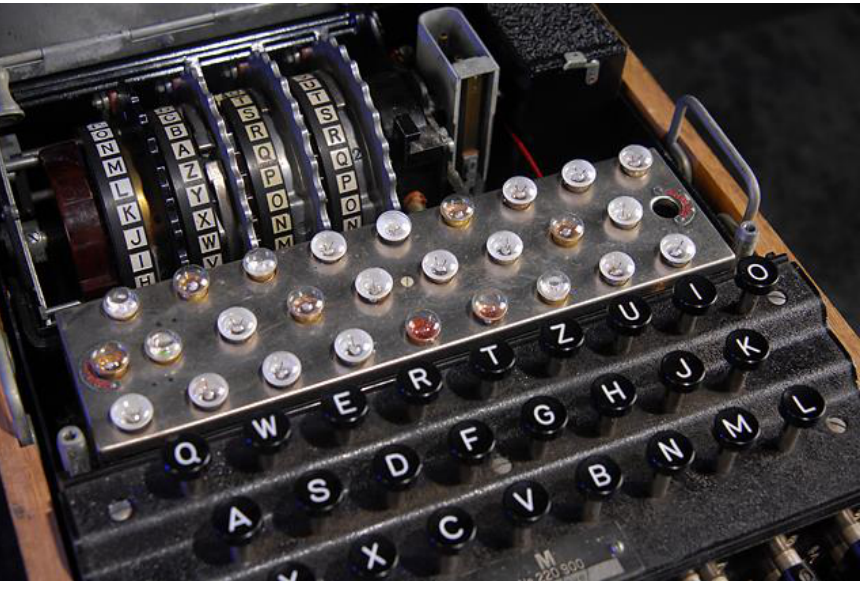
\includegraphics[width=94.71mm,height=162.16mm]{images/llm/page_111_img_01.png}%
\end{textblock*}

\newpage

% --- unit llm 112 ---
% === Halaman 112 (llm) ===

\begin{itemize}
  \item Sebagai contoh, tinjau 3 rotor yang disederhanakan menjadi hanya 6 huruf alfabet:
\end{itemize}

\vspace{5mm}

\begin{itemize}
  \item Misalkan huruf plainteks D ditekan pada keyboard
  \item Huruf D dienkripsi oleh roto pertama menjadi E
  \item Huruf E menjadi input untuk rotor kedua, dienkripsi menjadi B
  \item Huruf B menjadi input untuk rotor ketiga, dienkripsi menjadi E
  \item Jadi, huruf D dienkripsi menjadi E
\end{itemize}

\vspace{5mm}

\begin{itemize}
  \item Setelah D dienkripsi menjadi E, rotor ketiga bergeser satu huruf.
  \item Jika D dienkripsi kembali, maka hasilnya adalah A
\end{itemize}

\vspace{10mm}

Sumber: \url{https://www.usna.edu/Users/cs/nchamber/courses/ic211/s19/lab/l04/realenigma.html}

% deskripsi: Diagram alur enkripsi huruf D melalui tiga rotor (Rotor 1, Rotor 2, Rotor 3) yang menunjukkan pemetaan huruf dari satu rotor ke rotor berikutnya hingga hasil akhir E.
% bbox normalisasi: [0.0600, 0.1080, 0.9400, 0.9120]
\begin{textblock*}{184.80mm}(12.60mm,32.08mm)
\noindent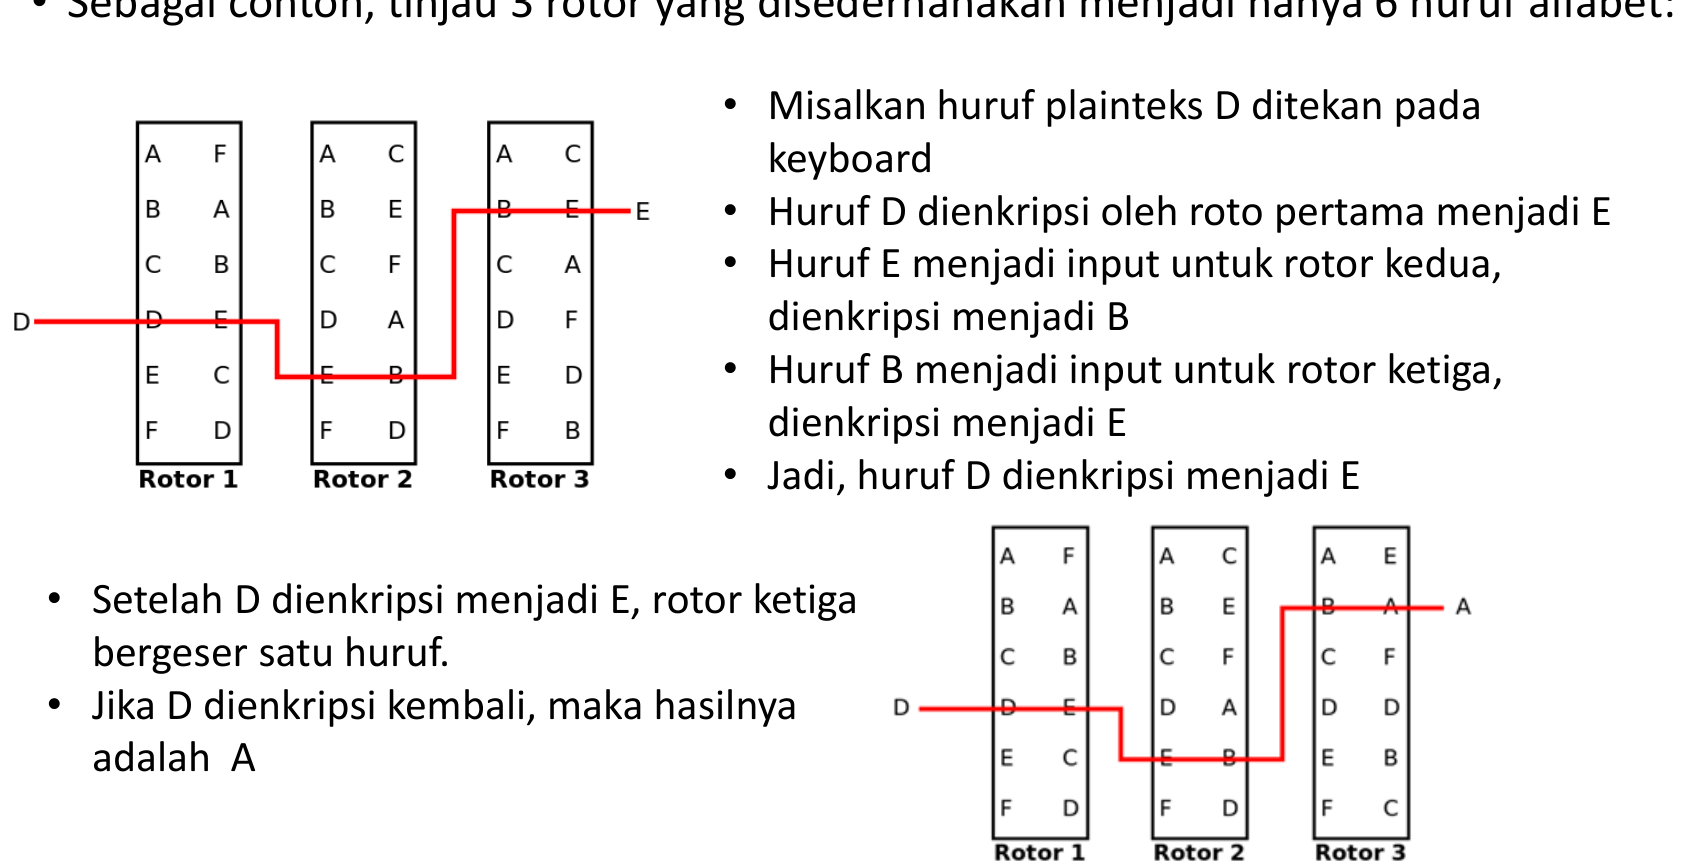
\includegraphics[width=184.80mm,height=238.79mm]{images/llm/page_112_img_01.png}%
\end{textblock*}

% deskripsi: Diagram alur enkripsi huruf D setelah rotor ketiga bergeser, menunjukkan pemetaan huruf yang berubah sehingga hasil akhirnya menjadi A.
% bbox normalisasi: [0.5200, 0.6000, 0.8300, 0.9000]
\begin{textblock*}{65.10mm}(109.20mm,178.20mm)
\noindent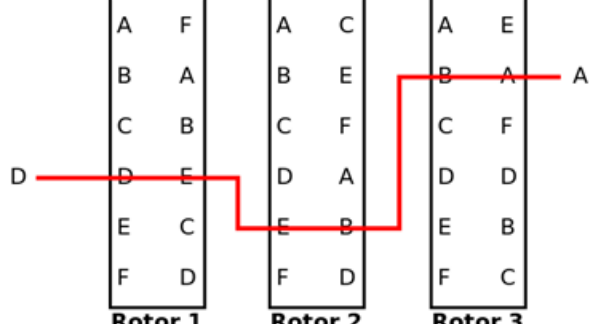
\includegraphics[width=65.10mm,height=89.10mm]{images/llm/page_112_img_02.png}%
\end{textblock*}

% bbox perkiraan otomatis: Diagram alur enkripsi huruf D melalui tiga rotor (Rotor 1, Rotor 2, Rotor 3) yang menunjukkan pemetaan huruf dari satu rotor ke rotor berikutnya hingga hasil akhir E.

\newpage

% --- unit llm 113 ---
% === Halaman 113 (llm) ===

\begin{itemize}
  \item Model mesin enigma ada yang menggunakan 3 rotor atau 4 rotor, setiap rotor melakukan operasi substitusi cipher abjad-tunggal.
  \item Untuk mesin enigma 4-rotor, berarti terdapat $26 \times 26 \times 26 \times 26 = 456.976$ kemungkinan huruf cipherteks sebagai pengganti huruf plainteks sebelum terjadi perulangan urutan cipherteks.
  \item Setiap kali sebuah huruf selesai disubstitusi, \textit{rotor} pertama bergeser satu huruf.
  \item Setiap kali \textit{rotor} pertama selesai bergeser 26 kali, rotor kedua bergeser satu huruf. Setelah rotor kedua bergeser 26 kali, rotor ketiga bergeser satu huruf. Setelah rotor ketiga bergeser 26 kali, rotor keempat bergeser satu huruf.
\end{itemize}

\newpage

% --- unit llm 114 ---
% === Halaman 114 (llm) ===

\begin{itemize}
    \item Posisi awal keempat \textit{rotor} dapat di-set; dan posisi awal ini menyatakan kunci dari Enigma.
    \item Kriptanalisis mesin Enigma pertama kali ditemukan pada tahun 1932 oleh kriptografer Polandia, yaitu Marian Rejewski, Jerzy Różycki dan Henryk Zygalski.
    \item Pemerintahan Nazi Jerman kemudian mendesain ulang mesin Enigma pada tahun 1939 dengan menambahkan \textbf{plugboard} dan \textbf{reflektor}, sehingga proses enkripsi menjadi lebih kompleks. Metode kriptanalisis Enigma sebelumnya tidak dapat digunakan lagi.
\end{itemize}

\vspace{44.55mm}

% deskripsi: Diagram skema kerja mesin Enigma yang menunjukkan aliran sinyal melalui Reflektor, Left Rotor, Middle Rotor, dan Right Rotor, mengilustrasikan proses enkripsi huruf A menjadi G dan A menjadi C.
% bbox normalisasi: [0.6050, 0.7500, 0.9900, 0.9000]
\begin{textblock*}{80.85mm}(127.05mm,222.75mm)
\noindent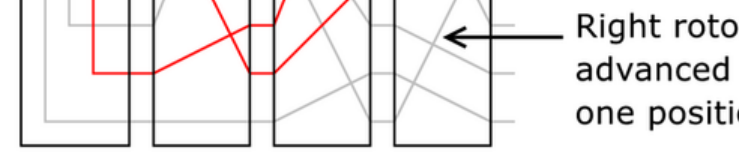
\includegraphics[width=80.85mm,height=44.55mm]{images/llm/page_114_img_01.png}%
\end{textblock*}

\newpage

% --- unit llm 115 ---
% === Halaman 115 (llm) ===

\vspace{166.32mm}

\begin{itemize}
    \item Jerman sangat percaya diri bahwa Enigma tidak akan dapat dipecahkan.
    \item Namun, dengan bantuan Polandia, Perancis dan Inggris kemudian membuat mesin pemecah Enigma baru ini, yang diberi nama \textit{bombe}.
    \item \textit{Bombe} dirancang oleh Alan Turing.
    \item \textit{Bombe} berhasil memecahkan Enigma Cipher buatan Jerman.
    \item Keberhasilan memecahkan Enigma Cipher dianggap sebagai faktor yang memperpendek perang dunia kedua menjadi hanya dua tahun.
\end{itemize}

\vspace{10mm}

Coba simulator online Enigma di: \url{https://www.101computing.net/enigma/enigma-instructions.html}

% deskripsi: Foto hitam putih mesin Bombe yang digunakan untuk memecahkan kode Enigma
% bbox normalisasi: [0.6110, 0.0930, 0.9560, 0.6530]
\begin{textblock*}{72.45mm}(128.31mm,27.62mm)
\noindent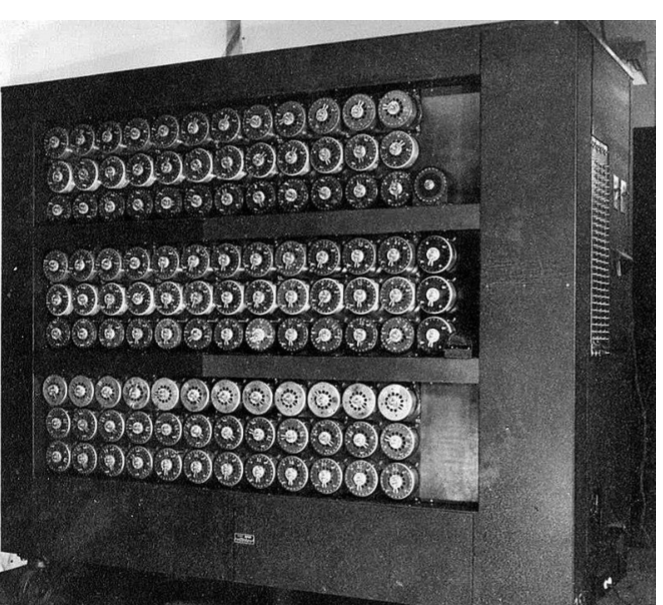
\includegraphics[width=72.45mm,height=166.32mm]{images/llm/page_115_img_01.png}%
\end{textblock*}

\newpage

% --- unit llm 116 ---
% === Halaman 116 (llm) ===

% (tidak ada teks dari model)

% deskripsi: Screenshot simulator mesin Enigma M3 yang menunjukkan keyboard, roda rotor, dan lampu indikator huruf.
% bbox normalisasi: [0.2110, 0.1570, 0.7580, 0.9530]
\begin{textblock*}{114.87mm}(44.31mm,46.63mm)
\noindent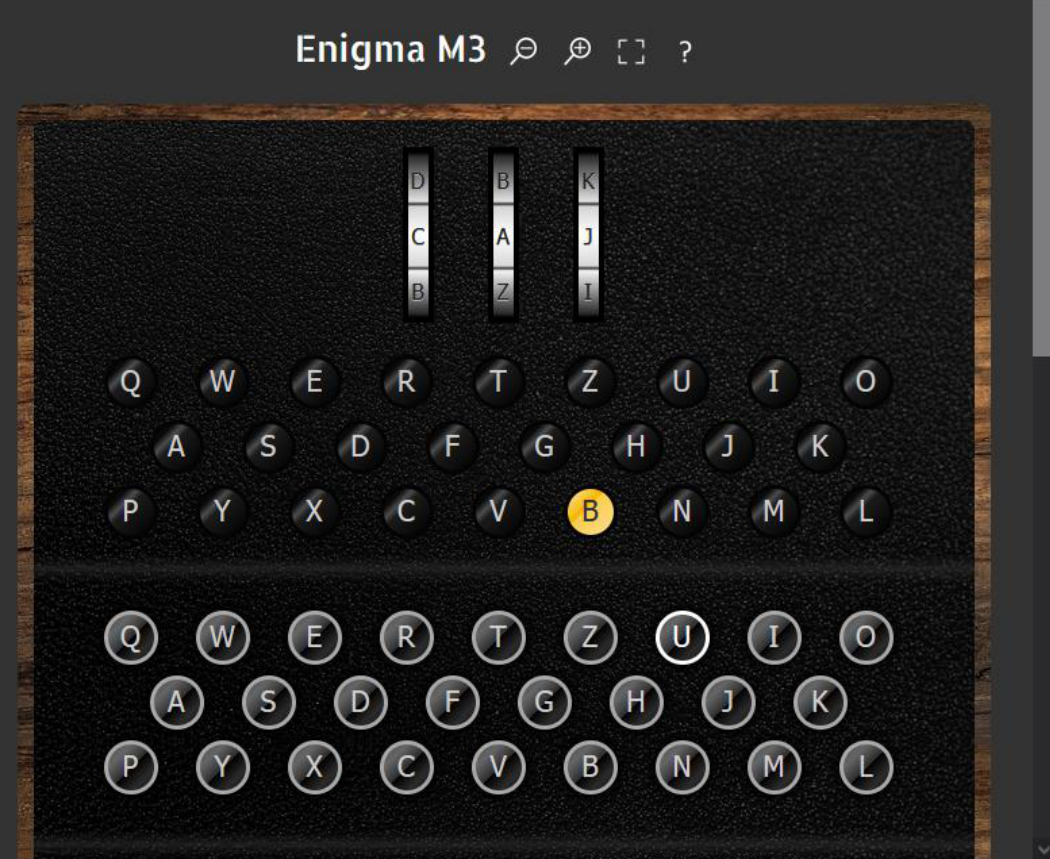
\includegraphics[width=114.87mm,height=236.41mm]{images/llm/page_116_img_01.png}%
\end{textblock*}

\newpage

% --- unit llm 117 ---
% === Halaman 117 (llm) ===

\vspace{214.14mm}

Plaintext:\\
PESAW ATMEN DARAT\\\vspace{5mm}
Ciphertext:\\
GUFYL FRKQE JXVHM

% deskripsi: Simulasi mesin Enigma yang menunjukkan keyboard, panel lampu indikator huruf, dan output teks plaintext serta ciphertext.
% bbox normalisasi: [0.3030, 0.1330, 0.6700, 0.8540]
\begin{textblock*}{77.07mm}(63.63mm,39.50mm)
\noindent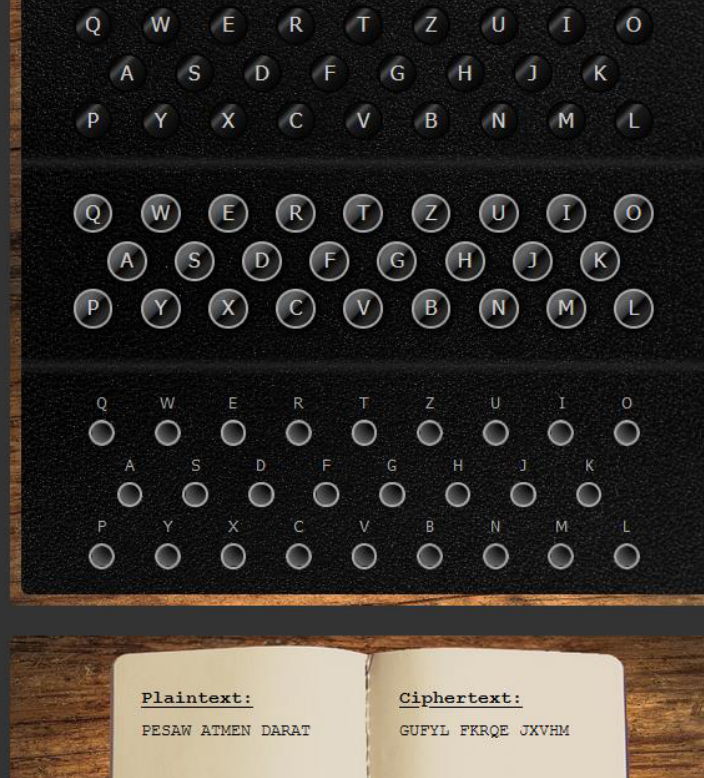
\includegraphics[width=77.07mm,height=214.14mm]{images/llm/page_117_img_01.png}%
\end{textblock*}

\newpage

% --- unit llm 118 ---
% === Halaman 118 (llm) ===

Encryption Steps:

\begin{tabular}{lll}
Keyboard Input: P & Keyboard Input: E & Keyboard Input: S \\
Rotors Position: ABE & Rotors Position: ABM & Rotors Position: ABG \\
Plugboard Encryption: P & Plugboard Encryption: E & Plugboard Encryption: S \\
Wheel 3 Encryption: W & Wheel 3 Encryption: W & Wheel 3 Encryption: K \\
Wheel 2 Encryption: U & Wheel 2 Encryption: U & Wheel 2 Encryption: G \\
Wheel 1 Encryption: A & Wheel 1 Encryption: A & Wheel 1 Encryption: D \\
Reflector Encryption: Y & Reflector Encryption: Y & Reflector Encryption: H \\
Wheel 1 Encryption: O & Wheel 1 Encryption: O & Wheel 1 Encryption: P \\
Wheel 2 Encryption: T & Wheel 2 Encryption: T & Wheel 2 Encryption: P \\
Wheel 3 Encryption: G & Wheel 3 Encryption: Q & Wheel 3 Encryption: F \\
Plugboard Encryption: G & Plugboard Encryption: Q & Plugboard Encryption: F \\
Output (Lampboard): G & Output (Lampboard): Q & Output (Lampboard): F \\
------------------- & ------------------- & -------------------
\end{tabular}

\newpage

% --- unit llm 119 ---
% === Halaman 119 (llm) ===

TAMAT

\end{document}
